% This LaTeX document needs to be compiled with XeLaTeX.
\documentclass[
  10
]{article}
\usepackage[margin=2cm,includehead=true,includefoot=true,centering,]{geometry}
\usepackage{xcolor}
\usepackage{ucharclasses}
\usepackage{xurl}  % allow URLs to break at any character
\usepackage{hyperref}
\usepackage{amsmath,amssymb}
\usepackage{amsfonts}
\usepackage[version=4]{mhchem}
\usepackage{stmaryrd}
\usepackage{bbold}
\usepackage{polyglossia}
\usepackage{fontspec}
\usepackage{ctex}
\usepackage[export]{adjustbox}

\usepackage{tabularx}
\usepackage{booktabs}

\usepackage{setspace}
\setstretch{1.2}

\makeatletter
\@ifundefined{KOMAClassName}{% if non-KOMA class
  \IfFileExists{parskip.sty}{%
    \usepackage{parskip}
  }{% else
    \setlength{\parindent}{0pt}
    \setlength{\parskip}{6pt plus 2pt minus 1pt}}
}{% if KOMA class
  \KOMAoptions{parskip=half}}
\makeatother
\usepackage{longtable,booktabs,array}
\usepackage{ragged2e}
\newcolumntype{L}[1]{>{\RaggedRight\arraybackslash}p{#1}}
\newcounter{none} % for unnumbered tables
\usepackage{multirow}
\usepackage{calc} % for calculating minipage widths
% Correct order of tables after \paragraph or \subparagraph
\usepackage{etoolbox}
\makeatletter
\patchcmd\longtable{\par}{\if@noskipsec\mbox{}\fi\par}{}{}
\makeatother
% Allow footnotes in longtable head/foot
\IfFileExists{footnotehyper.sty}{\usepackage{footnotehyper}}{\usepackage{footnote}}
\makesavenoteenv{longtable}
\usepackage{graphicx}
\makeatletter
\newsavebox\pandoc@box
\newcommand*\pandocbounded[1]{% scales image to fit in text height/width
  \sbox\pandoc@box{#1}%
  \Gscale@div\@tempa{\textheight}{\dimexpr\ht\pandoc@box+\dp\pandoc@box\relax}%
  \Gscale@div\@tempb{\linewidth}{\wd\pandoc@box}%
  \ifdim\@tempb\p@<\@tempa\p@\let\@tempa\@tempb\fi% select the smaller of both
  \ifdim\@tempa\p@<\p@\scalebox{\@tempa}{\usebox\pandoc@box}%
  \else\usebox{\pandoc@box}%
  \fi%
}
% Set default figure placement to htbp
\def\fps@figure{htbp}
\makeatother
\sloppy
\setlength{\emergencystretch}{3em} % prevent overfull lines
\providecommand{\tightlist}{%
  \setlength{\itemsep}{0pt}\setlength{\parskip}{0pt}}


\hypersetup{colorlinks=true, linkcolor=blue, filecolor=magenta, urlcolor=cyan,}
\urlstyle{same}

\usepackage{colortbl}
\definecolor{table-row-color}{HTML}{999999}
\definecolor{table-rule-color}{HTML}{999999}
%\arrayrulecolor{black!40}
\arrayrulecolor{table-rule-color}     % color of \toprule, \midrule, \bottomrule
\setlength{\aboverulesep}{0pt}
\setlength{\belowrulesep}{0pt}


\setotherlanguages{english}
\IfFontExistsTF{Songti SC}
{\newfontfamily\chinesefont{Songti SC}}
{\IfFontExistsTF{Source Han Serif CN}
{\newfontfamily\chinesefont{Source Han Serif CN}}
{\IfFontExistsTF{Noto Serif CJK SC}
  {\newfontfamily\chinesefont{Noto Serif CJK SC}}
  {\IfFontExistsTF{SimSun}
    {\newfontfamily\chinesefont{SimSun}}
    {\IfFontExistsTF{FangSong}
      {\newfontfamily\chinesefont{FangSong}}
      {\newfontfamily\chinesefont{Arial Unicode MS}}
}}}}
\setCJKmainfont{Songti SC}
\setCJKsansfont{Heiti SC}

\IfFontExistsTF{Times New Roman}
{\newfontfamily\englishfont{Times New Roman}}
{\IfFontExistsTF{Liberation Serif}
  {\newfontfamily\englishfont{Liberation Serif}}
  {\IfFontExistsTF{DejaVu Serif}
    {\newfontfamily\englishfont{DejaVu Serif}}
    {\newfontfamily\englishfont{Arial}}
}}


\author{}
\date{}

\begin{document}

\renewcommand{\figurename}{图}
\renewcommand{\tablename}{表}




\begin{center}
{\LARGE DeepSeek-V4.1-Flash\par}
\vspace{0.5em}
{\large 突破 KV 缓存压缩的极限\par}
\vspace{0.8em}
{\normalsize DeepSeek-AI\quad research@deepseek.com\par}
\end{center}
\label{deepseek-v4.1-flash-pushing-the-limits-of-kv-cache-compression}



\renewcommand{\contentsname}{目录}
\tableofcontents
\clearpage
\section*{摘要}\label{abstract}

长程智能体的广泛采用使模型工作负载日益呈现出输入密集（input-heavy）的特征。尽管已有
工作大幅降低了长上下文计算的开销，预填充（prefill）阶段的计算成本仍然高昂，且庞大的
KV 缓存持续给 HBM 与 SSD 容量以及数据传输带宽带来压力。计算、存储与带宽三方面的
需求共同构成了进一步降低部署成本的主要瓶颈。为应对这一挑战，我们提出了
DeepSeek-V4.1-Flash：一个多模态混合专家（Mixture-of-Experts，MoE）模型，主干参数
规模为 552B，支持最长一百万 token 的上下文。凭借其因果编码器-解码器
（Causal Encoder-Decoder，CED）架构，模型在解码阶段每 token 激活 16B 参数，
在预填充阶段则仅激活 8B 参数，显著提升了智能体工作负载的成本效率。为突破 KV
缓存压缩的极限，DeepSeek-V4.1-Flash 在压缩稀疏注意力 2（Compressed Sparse
Attention 2，CSA2）中结合了跨层 KV 缓存复用，并采用 FP4 KV 缓存。这些设计将其
全局 KV 缓存占用（始终驻留于 HBM）降至每 token 890 字节，约为 DeepSeek-V4-
Flash 相应占用的 1/4。此外，通过一项名为 SWA Bounded Replay 的专用部署优化，
DeepSeek-V4.1-Flash 将其持久化 KV 缓存占用（始终驻留于 SSD 或主机内存）降至
DeepSeek-V4-Flash 的约 1/8。尽管 KV 缓存占用大幅减小，该模型仍取得了比基线明显
更优的性能。此外，我们对 DeepSeek-V4 的架构进行了精简，并引入了多项高效的架构
扩展。我们在包含 45T token 的多模态语料上对 DeepSeek-V4.1-Flash 进行预训练，并
开展全面的后训练，在多种纯文本与多模态智能体场景中均取得了强劲的性能。模型检查点
可在 https://huggingface.co/deepseek-ai/DeepSeek-V4.1-Flash 获取。

\section{引言}\label{introduction}

近年来，长程智能体的应用迅速扩展，使超长上下文处理成为日益重要的模型工作负载。
支持此类工作负载不仅需要高效的长序列处理，还需要对大型 KV 缓存进行持久化存储、
复用与迁移。因此，KV 缓存管理已成为模型部署的一项基础能力，同时也给计算、存储与
通信带来了巨大挑战。此前在稀疏注意力方面的进展 (DeepSeek-AI, 2025, 2026b) 显著
降低了长序列处理的计算成本，使持久化存储与数据搬运日益成为突出的瓶颈。

具体而言，DeepSeek-V4 (DeepSeek-AI, 2026b) 将覆盖整个上下文的全局注意力分支与
局部滑动窗口注意力（Sliding-Window Attention，SWA）相结合。全局分支维护全局 KV，
包括主 KV 与索引器 K，而 SWA 维护局部 KV 状态。在窗口大小固定的情况下，SWA 的
KV 存储量有界，与序列长度无关。因此，对于足够长的序列，全局 KV 主导了运行时 KV
占用，而后者受限于 HBM 容量。此外，部分 KV 会被持久化以用于前缀复用，称之为持久化
KV 缓存，其受限于 SSD 与主机内存容量。I/O 与互连带宽同样限制了缓存的迁移与加载。
这些约束共同限制了服务吞吐，推高了部署成本，并最终阻碍了智能体在更长任务周期与
更广泛应用场景中的部署与采用。

因此，进一步减小 KV 缓存占用对于缓解存储与通信瓶颈、降低长上下文服务成本至关重要。
为此，我们开发了 DeepSeek-V4.1-Flash：一个面向更激进 KV 缓存压缩而设计的多模态
混合专家（MoE）模型。DeepSeek-V4.1-Flash 拥有 552B 主干参数，原生支持多模态输入，
可容纳最长一百万 token 的上下文。我们采用因果编码器-解码器（CED）架构，解码器全局
KV 由编码器最终隐藏状态投影得到。该设计使模型在预填充阶段每 token 激活 8B 参数，
解码阶段激活 16B 参数，对输入密集的智能体场景尤为经济高效。尽管
DeepSeek-V4.1-Flash 明显大于 DeepSeek-V4-Flash，但在相同序列长度下，其所需的运行时
KV 缓存存储仅为后者的约 1/4，持久化 KV 缓存存储仅为后者的 1/8。此外，
DeepSeek-V4.1-Flash 的整体性能也优于 DeepSeek-V4-Flash。

这一程度的 KV 缓存压缩通过模型架构、缓存精度与部署策略三个方面的联合优化实现。从
概念上讲，DeepSeek-V4 可视为一个基于 SWA 的局部处理主干，辅以压缩后的全局上下文。
这一视角促使我们专注于简化全局分支，同时大体保留局部注意力设计。在架构层面，我们
设计了压缩稀疏注意力 2（Compressed Sparse Attention 2，CSA2），对全局 KV（包括
主 KV 与索引器 K）及 Top-K 索引采用跨层复用，从而大幅减少 KV 缓存存储。CSA2 有三
种静态分配的模式：Full、Reindex 与 Reuse。Full 模式生成全局 KV 并执行索引；Reindex
模式复用前一层的全局 KV，并使用自身的索引器 Q 对共享的索引器 K 重新打分，选出全新
的 Top-K 索引；Reuse 模式同时复用前一层的全局 KV 与 Top-K 索引，直接执行稀疏
注意力。三种模式下，每一层都保留自身的全局 Q 与 SWA KV。共享全局 KV 与索引器 K
减少了重复的缓存存储。此外，与采用压缩稀疏注意力（Compressed Sparse Attention，
CSA）与重度压缩注意力（Heavily Compressed Attention，HCA）混合架构的
DeepSeek-V4 不同，DeepSeek-V4.1-Flash 使用纯 CSA2。在缓存精度层面，我们在训练期间
使用 FP4 全局 KV 缓存，仅带来极小的性能损失。综上，CSA2 与 FP4 KV 缓存将全局 KV
缓存存储降至 DeepSeek-V4-Flash 的约 1/4，如图 1(b) 所示。在部署层面，与
DeepSeek-V4 相同，DeepSeek-V4.1-Flash 在每一层都使用滑动窗口注意力（SWA）。在
DeepSeek-V4 中，我们采用混合策略，在持久化 SWA KV 缓存的存储成本与精确重建所需
计算量之间进行权衡。精确重建需要重放最近
\(L \times n _ { \mathrm { w i n } }\) 个 token，其中 $L$ 为层数，
\(n _ { \mathrm { w i n } }\) 为 SWA 窗口大小。在 DeepSeek-V4.1-Flash 中，我们引入了
SWA Bounded Replay，仅重放最近 \(n _ { \mathrm { w i n } }\) 个 token 即可近似重建
所需的 SWA KV 状态。实验表明，这仅会造成可以忽略的性能损失。这一发现确立了一种新的
存储--计算权衡，使我们无需将 SWA KV 缓存持久化到 SSD，代价仅是一小部分预填充重算。
借助 SWA Bounded Replay，持久化 KV 缓存占用进一步降至 DeepSeek-V4-Flash 的约 1/8。
这些优化共同大幅缓解了 HBM 与 SSD 容量压力，降低了部署成本，并为更大规模的部署
铺平了道路。




作为 CED 与 CSA2 的补充，我们进一步精简了原有的 DeepSeek-V4 架构。此外，我们将原有
的 mHC (Xie et al., 2026) 设计升级为 Single-Pass mHC，并配套 Mega-mHC 部署内核，
与原有的四内核实现相比，激活内存访问量减半。进一步地，我们集成 Engram
(Cheng et al., 2026b) 条件记忆模块以增强模型能力。我们还引入了 DSpark
(Cheng et al., 2026a) 推测解码架构，通过半自回归草稿生成与置信度调度的验证来提高
解码效率。综合全部架构改进后，DeepSeek-V4.1-Flash 的单 token 解码 FLOPs 在不同
上下文长度下基本保持恒定。如图 2 所示，将上下文长度从 4K 扩展 256 倍至 1M，其解码
FLOPs 仅增加 1/4，远低于 DeepSeek-V4-Flash 的增长幅度。

为充分实现上述架构设计的 KV 缓存压缩收益，并进一步提升训练与推理效率，我们对
DeepSeek-V4.1-Flash 的训练基础设施与推理系统进行了系统性联合优化，确保大规模多模态
训练与长上下文部署既高效又可扩展。训练基础设施支持视觉编码器的解耦执行、长序列下
均衡的图像分片，以及用于注意力复用的跨阶段共享状态管理。推理系统实现了编码器
（Encoder）与解码器（Decoder）的 SWA Bounded Replay 路径。进一步的优化包括通信--
计算重叠、分片（sharded）的 Engram 嵌入表以及推理内核融合。特别地，每个 CSA2 Reuse
模式层在预填充阶段仅需执行 15 个内核，解码阶段仅需 11 个。我们还将主机内存中长
生命周期的全局 KV 存储与短生命周期的编码器 SWA KV 分开，利用有界重放（bounded
replay）近似重建缺失的编码器 SWA 状态。



在预训练阶段，我们在包含 45T token 的大规模多模态语料上训练 DeepSeek-V4.1-Flash。
稀疏注意力以 64K 的序列长度从头开始训练，没有经过任何密集注意力暖机（warmup）阶段。
预训练之后，模型具备原生的多模态能力，并支持最长一百万 token 的上下文。在我们的评估
中，DeepSeek-V4.1-Flash-Base 取得了与 DeepSeek-V4-Pro-Base 相当的世界知识、推理与
编码能力，在保留集（held-out）评估上提升 5\%--10\%，而总参数仅为后者的 1/3，激活
参数仅为 1/4。这些结果共同凸显了其强大的参数效率，也反映了训练数据质量面向真实部署
的改进。

在此基础模型之上，我们开展后训练以激发其推理与智能体能力。与上述架构创新不同，我们
的后训练没有引入任何算法层面的创新：配方沿用监督微调（Supervised Fine-Tuning，SFT）、
强化学习（Reinforcement Learning，RL）与同策略蒸馏（On-Policy Distillation，OPD）
的标准范式，除 DeepSeek-V4 开发中已经成熟的实践（DeepSeek-AI, 2026b）外未作任何
修改。所有实质性的改动都集中在数据流水线上。我们开发了用于数据合成与环境构建的大规模
自动化流水线，并逐步扩大 RL 阶段采用的数据、任务与 rollout 规模，从而将模型能力扩展
至文本、多模态与智能体等领域。图 1(a) 总结了 DeepSeek-V4.1-Flash 在核心智能体基准上
的性能。评估表明，尽管体型紧凑，DeepSeek-V4.1-Flash 仍展现出一套独特的能力画像：

• 推理。该模型具备强大的推理能力，在数学与竞技编程等推理密集型基准上保持高准确率，
与 Kimi-K3 (Team et al., 2026a) 和 DeepSeek-V4-Pro 等顶尖开源模型表现相当。

• 智能体。在 Terminal-Bench 2.1 (Merrill et al., 2026)、DeepSWE v1.1 (DataCurve,
2026) 和 AutomationBench (Shepard and Salimans, 2026) 等标准智能体基准上，
DeepSeek-V4.1-Flash 取得了与闭源前沿模型相当的性能。它已被证明完全能够胜任日常编码
任务与白领工作流。然而，在 Terminal-Bench 4.0 (Marten et al., 2026a) 等需要专家级
领域知识的科研型智能体任务上，与超大模型之间仍存在差距。

• 多模态。在多模态领域，该模型在评估视觉推理与专业图表解读的基准上尤其超越 Kimi-K3
等顶尖开源竞品。除正式指标外，它在现实世界的视觉智能体工作流中也展现出实际用途，例如
前端开发与办公自动化——它可以利用渲染后的屏幕截图进行视觉检查与自我修正。尽管如此，
我们承认，与大型闭源系统相比仍存在明显的整体性能差距。

这些结果表明，DeepSeek-V4.1-Flash 在绝大多数基准上已能与闭源前沿模型匹敌，并且能够
完成超过 95\% 的现实世界任务。与此同时，其较小的激活占用带来了较低的推理延迟与服务
成本。因此我们相信，DeepSeek-V4.1-Flash 在能力与效率之间提供了良好的权衡，能够作为
一位快速、实惠的助手，服务广大用户的日常工作。总而言之，DeepSeek-V4.1-Flash 在提升
模型智能与推理效率的同时降低了部署成本。它大幅降低了大规模部署长程智能体的成本门槛，
并为其在更广泛场景中的应用创造了新的机会。DeepSeek-V4.1-Flash 也为我们持续的规模化
扩展提供了新的起点。在此基础之上，我们将继续推进模型架构、预训练与后训练的联合规模化
扩展，以进一步探索模型智能的前沿。




\begin{figure}[htbp]
\centering
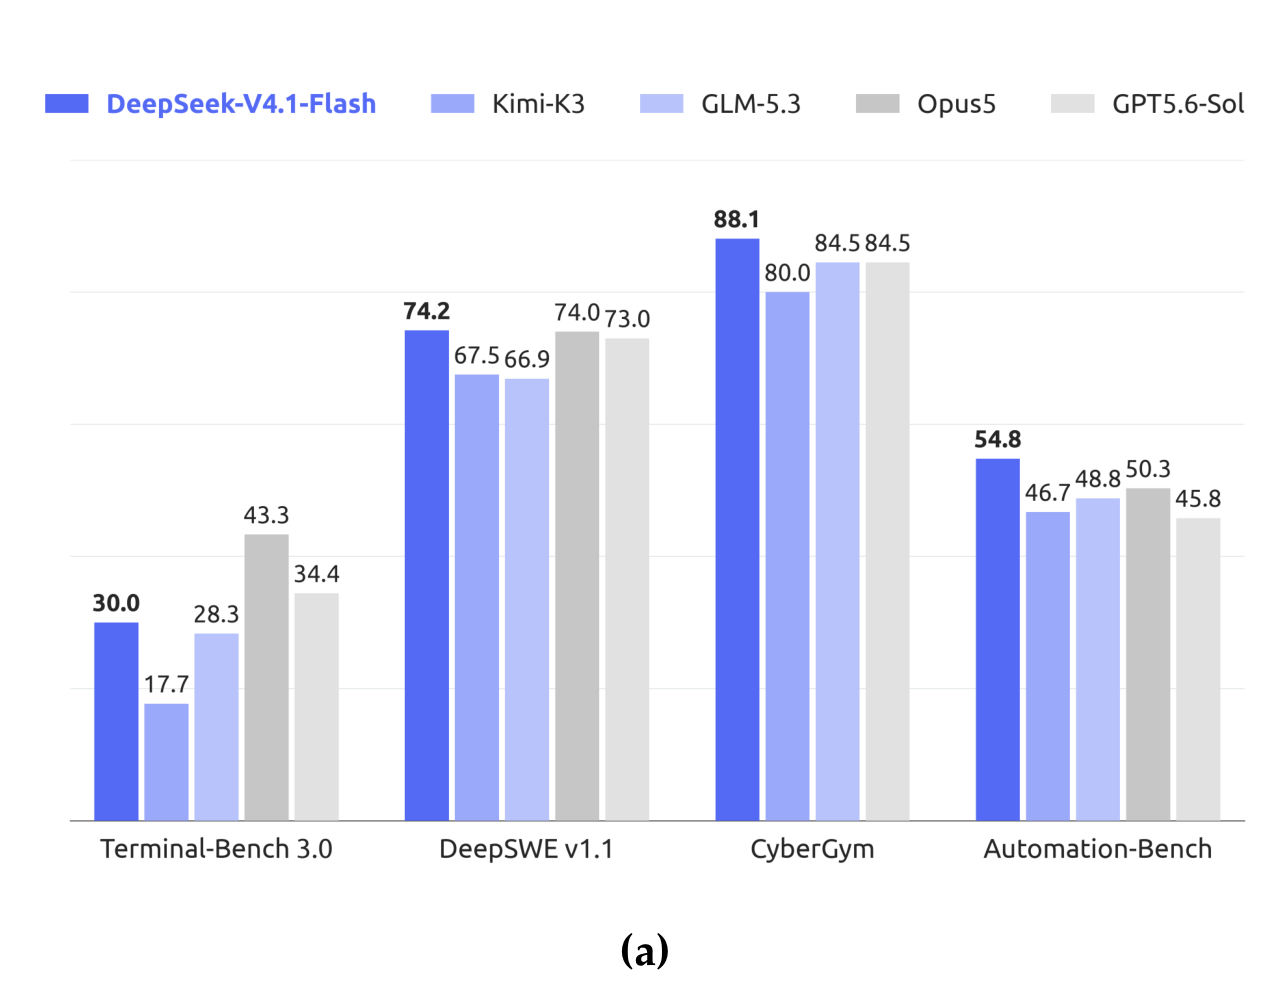
\includegraphics[width=0.48\linewidth]{images_hi/fig01a}
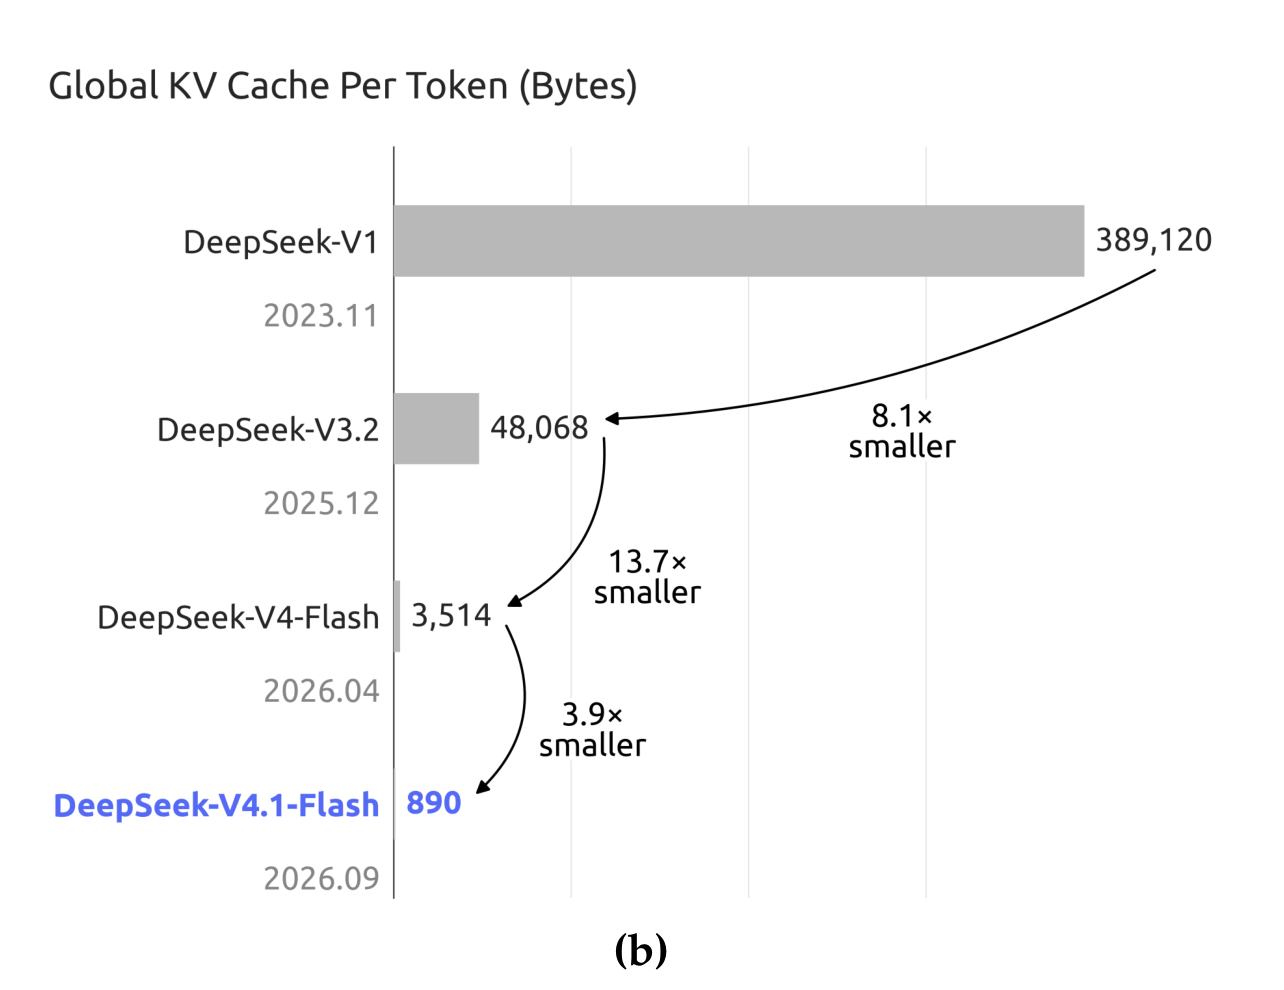
\includegraphics[width=0.48\linewidth]{images_hi/fig01b}
\hfill
\caption{(a) DeepSeek-V4.1-Flash 及其对标模型在智能体基准上的性能。(b) 历代 DeepSeek 模型的每 token 全局 KV 缓存大小（字节），凸显了 DeepSeek 在降低上下文内存需求方面的持续努力。与 DeepSeek-V4-Flash 和 DeepSeek-V1 相比，DeepSeek-V4.1-Flash 的每 token 全局 KV 缓存大小分别实现了约 4 倍与 437 倍的缩减。}
\label{fig:1}
\end{figure}
\begin{figure}[htbp]
\centering
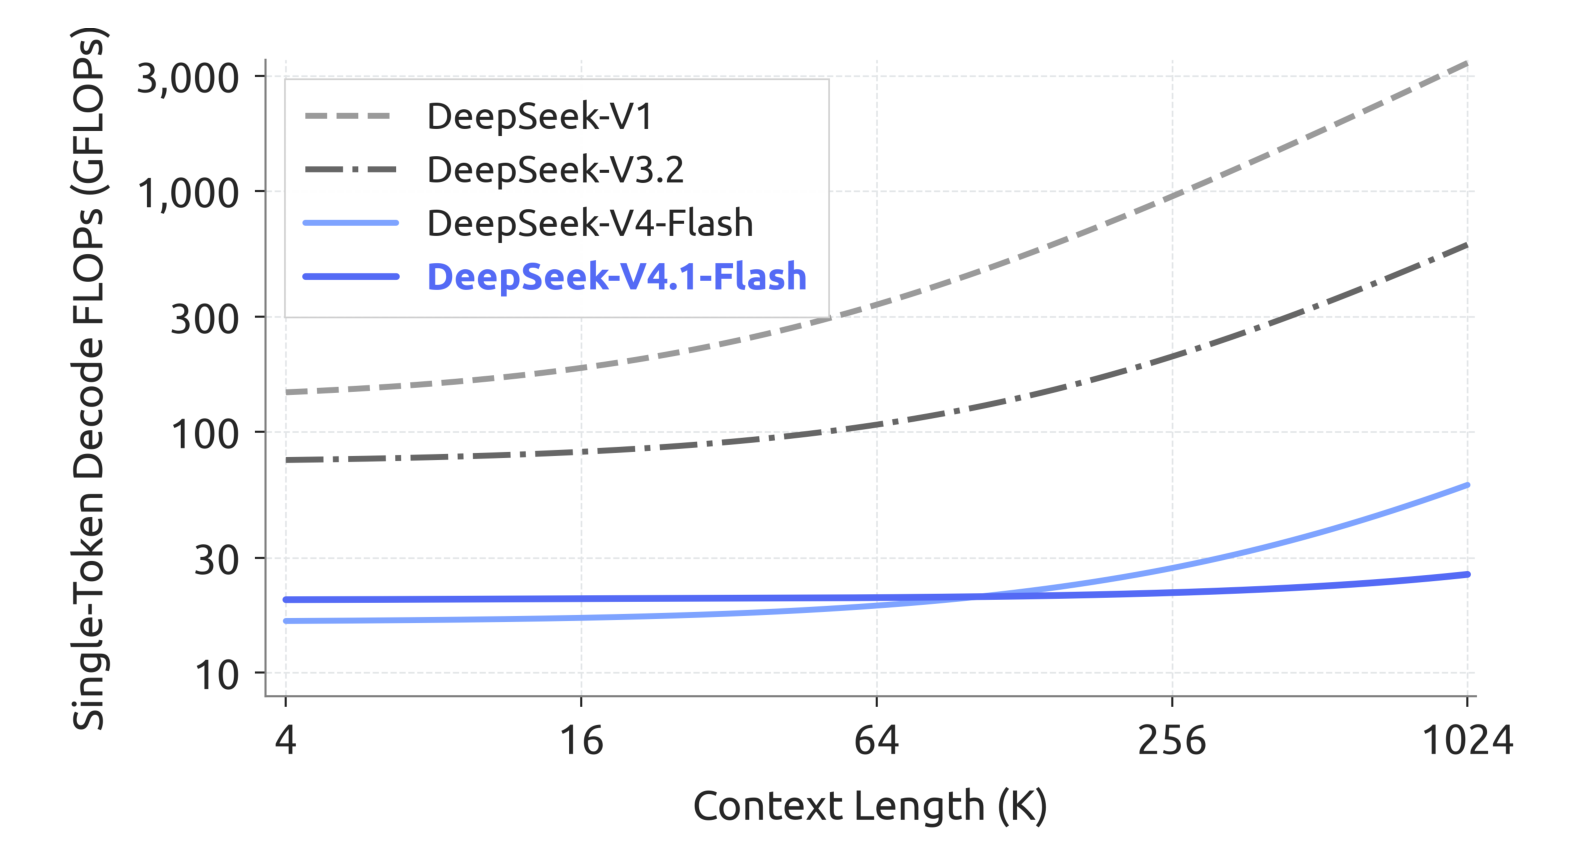
\includegraphics[width=\linewidth]{images_hi/fig02}
\caption{历代 DeepSeek 模型的单 token 解码 FLOPs 随上下文长度的变化。我们按 1、0.5、0.25 分别加权 BF16、FP8 与 FP4 运算，以计入计算精度差异。随着上下文长度增加，DeepSeek-V4.1-Flash 的解码 FLOPs 基本保持恒定，大幅降低了长上下文场景的计算成本。}
\label{fig:2}
\end{figure}
\begin{figure}[htbp]
\centering
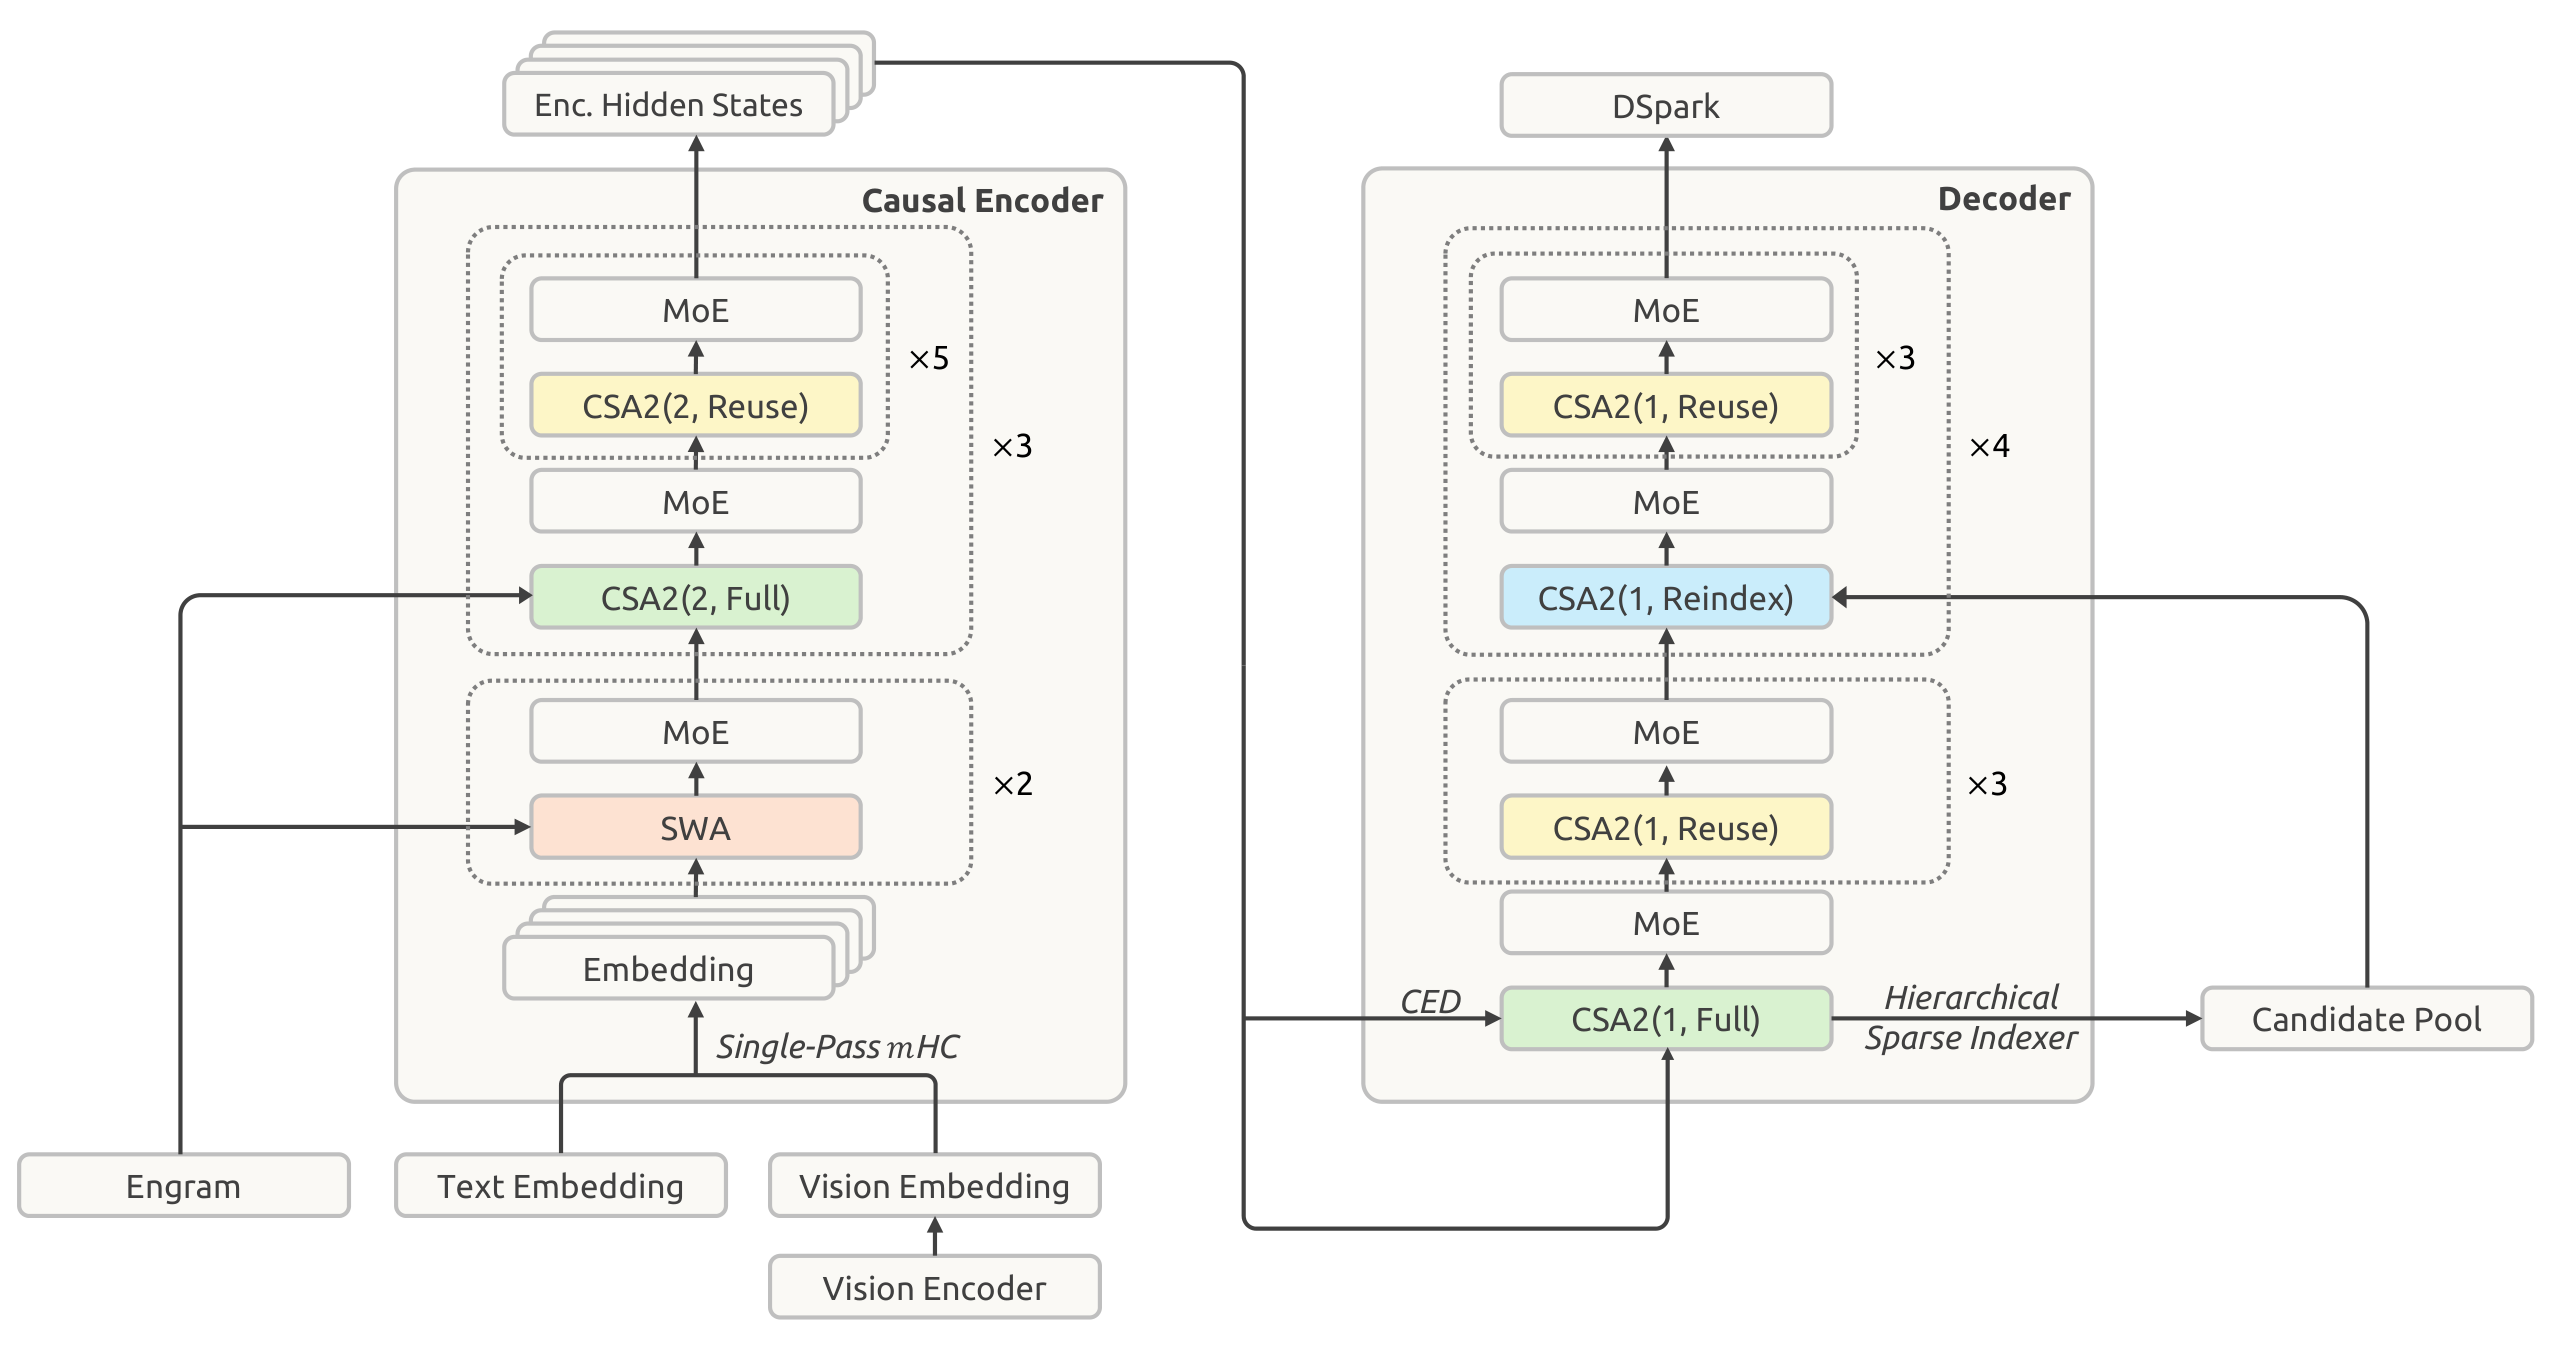
\includegraphics[width=\linewidth]{images_hi/fig03}
\caption{DeepSeek-V4.1-Flash 的整体架构。40 层网络分为因果编码器与解码器两部分，各含 20 层。所有前馈层均使用标准 DeepSeekMoE。前两层编码器使用滑动窗口注意力（SWA），其余层使用压缩稀疏注意力 2（CSA2），其中 CSA2(ratio, mode) 用于指定压缩率与模式。该模型还使用了 Single-Pass mHC、Engram、DSpark 与层级稀疏索引器（Hierarchical Sparse Indexer）。}
\label{fig:3}
\end{figure}
\section{架构}\label{architecture}

\subsection{概览}\label{overview}

DeepSeek-V4.1-Flash 是一个多模态混合专家（MoE）Transformer，以图像和文本作为输入，并以自回归方式生成文本。其语言主干由 40 层因果 Transformer 层组成，组织为一个 20 层因果编码器后接一个 20 层解码器。除前两层仅使用滑动窗口注意力（SWA）外，每一层都同时包含全局注意力和滑动窗口注意力。视觉编码器和 MLP 投影器将图像转换为视觉嵌入，与文本嵌入联合处理，多模态数据从语言模型预训练之初即被纳入。总体而言，DeepSeek-V4.1-Flash 拥有 552B 主干参数和 196B Engram 参数，预填充阶段每个 token 激活 8B 参数，解码阶段激活 16B 参数。图 3 展示了 DeepSeek-V4.1-Flash 的整体架构。

因果编码器--解码器（CED）架构与压缩稀疏注意力 2（CSA2）



共同解决长上下文推理中的互补性成本。CED 从编码器输出构建解码器的全局键值（KV）缓存，使大多数提示词 token 可以绕过完整的解码器计算，同时保留逐层局部的滑动窗口注意力。这几乎将预填充计算量减半，降低了在上下文不断增长的智能体工作负载中处理新输入或未缓存输入的成本。CSA2 跨层共享全局 KV 以降低缓存存储，并复用稀疏选择以减少索引工作量。在解码器中，分层稀疏索引器（Hierarchical Sparse Indexer）将后续索引器限制在由更早的索引器选出的候选池内，从而进一步减少每个查询需要计分的条目数量。

我们保留了 DeepSeekMoE（Dai et al., 2024）的共享专家和细粒度路由专家，并为图像和文本 token 引入了模态特定的负载均衡（Wang et al., 2024a）。Single-Pass mHC（Xie et al., 2026）改进了残差流混合方式，以实现更高效的核融合，Engram（Cheng et al., 2026b）则增加了可稀疏访问的条件记忆。我们在主干预训练期间省略了 MTP 模块，并使用 DSpark（Cheng et al., 2026a）进行推测解码。我们在主干预训练阶段之后单独训练 DSpark。此外，我们将主 KV 缓存压缩为 FP4，以进一步减少存储开销。以下各节介绍这些组件及相应的优化改动。

\subsubsection{多模态架构}\label{multimodal-architecture}

多模态输入通路由一个视觉编码器和一个 MLP 投影器组成。对于每张输入图像，视觉编码器都会生成一个视觉特征的空间网格。随后，一个 3 $\times$ 3 的 pixel-unshuffle 操作沿通道维度重排每个局部邻域，在 MLP 投影器将特征映射到语言主干的隐藏维度之前降低空间分辨率。最后，得到的视觉嵌入会被插入到输入嵌入序列中对应图像 token 的位置，并由语言主干与文本嵌入联合处理。

DeepSeek-ViT 我们从零开始训练了一个名为 DeepSeek-ViT 的视觉编码器，使其能够原生处理不同分辨率的图像。我们在 Vision Transformer（Dosovitskiy et al., 2021）架构的基础上构建 DeepSeek-ViT，并做了若干修改。为容纳任意分辨率的输入，我们用 2D-RoPE 替换了标准的绝对位置嵌入。为使 ViT 更贴近 LLM 的设计原则，我们将 patch 嵌入层的卷积替换为线性投影，以确保与 Muon 优化器兼容。我们还采用 RMSNorm（Zhang and Sennrich, 2019）进行归一化，并使用 SwiGLU（Shazeer, 2020）作为激活函数。在将视觉特征送入 LLM 之前，我们应用一个 3 $\times$ 3 下采样的 pixel-unshuffle 操作，将视觉 token 数量减少为原来的九分之一，从而有效支持高达约 1344 $\times$ 1344 像素的输入分辨率。

多模态 MoE 的无辅助损失负载均衡 图像 token 与文本 token 表现出不同的表征分布，可能在 MoE 中诱发不同的专家路由偏好。因此，平衡它们的总体负载可能会掩盖模态特定的不均衡。为解决这一问题，我们扩展了无辅助损失负载均衡（Wang et al., 2024a），为文本和图像 token 分别维护独立的按专家修正偏置。在路由过程中，每个 token 使用与其模态关联的修正偏置进行专家选择，同时保留原始路由分数用于对所选专家输出进行加权。每个训练步骤之后，两组偏置根据各自的专家负载独立更新。这一设计平衡了每种模态内部的专家利用率，有助于稳定高效的多模态训练。



\subsection{因果编码器-解码器（CED）}\label{causal-encoder-decoder-ced}

在智能体工作流中，频繁的工具调用会产生大量预填充请求，当 KV 缓存未命中时会带来严重的计算开销。为缓解这一预填充瓶颈，我们提出了因果编码器-解码器（CED）架构，其灵感来自 YoCo（Sun et al., 2024）。YoCo 通过允许上层一半的层直接共享下层一半的层生成的 KV 缓存来减少预填充计算。在此基础上，CED 引入了一系列结构性改进，以同时提升整体 KV 缓存容量和 KV 生成的计算深度。因此，CED 在保持与基线相当性能的同时，成功将预填充计算量减少了近一半。

对于全局注意力，CED 将 Transformer 的底部 \(L / 2\) 层视为因果编码器。对于上层一半的层（即解码器，\(l > L / 2 )\) ），KV 条目并非直接来自它们各自的隐藏状态 \(H _ { l } .\) 。相反，它们是使用随层变化的投影权重 \(( \dot { W } _ { l } ^ { K V }\) 和 \(W _ { l } ^ { Z } )\) 从第 \(( L / 2 )\) 层的隐藏状态 \(H _ { L / 2 }\) 投影得到的：

\[
C _ { l } = H _ { L / 2 } W _ { l } ^ { K V } , \quad Z _ { l } = H _ { L / 2 } W _ { l } ^ { Z } , \quad l > \frac { L } { 2 } ,\tag{1}
\]

其中 $C$ 与 $Z$ 分别表示 KV 条目及其对应的压缩权重。这一设计使 CED 在预填充阶段只需计算前一半的层，便能以极小的计算量获得上层的全局 KV 缓存。

对于滑动窗口注意力（SWA），CED 在所有层中保持传统的逐层计算。具体而言，对于任意层 $l$，局部键和值直接从当前层的隐藏状态 \(H _ { l } .\) 得出。这一设计有效增加了局部 KV 生成的计算深度。然而，保持这种逐层计算需要一次 SWA 重放（replay）过程。在预填充阶段，为解码器计算 SWA KV 缓存需要额外处理 \(n _ { \mathrm { w i n } } \times L / 2\) 个 token（其中 \(n _ { \mathrm { { w i n } } }\) 表示窗口大小）。对于每轮提示都很短的多轮交互，解码器中的这一计算开销变得不可忽略。幸运的是，先前的工作（Chen et al., 2025）已经表明，SWA 的实际有效感受野远小于理论上的 \(n _ { \mathrm { w i n } } \times L / 2\)。受此启发，我们引入了 Decoder SWA Bounded Replay，它只为 SWA 计算预填充提示中最后 \(n _ { \mathrm { w i n } }\) 个 token，从而显著降低计算成本。更多细节见第 3.2.2 节。

总体而言，对于序列长度 \(N \gg n _ { \mathrm { w i n } } ,\) CED 将预填充复杂度从 \(O ( N L )\) 降低为 \({ \cal O } ( N L / 2 + n _ { \mathrm { w i n } } \times L / 2 ) \approx { \cal O } ( N L / 2 )\)，实际将整体计算量减半。

\subsection{压缩稀疏注意力 2（CSA2）}\label{compressed-sparse-attention-2-csa2}

服务长上下文需要同时控制 KV 缓存存储和注意力计算。这些成本可以从三个乘性维度加以降低：条目大小维度，其中 GQA（Ainslie et al., 2023）减少了 KV 头的数量，MLA（DeepSeek-AI, 2024）在各头之间共享一个小型的潜在向量；序列维度，其中每 $m$ 个 token 被压缩成一个条目，如 DeepSeek-V4（DeepSeek-AI, 2026b）中的 CSA 和 HCA；以及层维度，其中一些层复用其他层的缓存（Brandon et al., 2024）和选择结果，而非保留自己的缓存，或者干脆被替换为更高效的层。先前的工作表明，沿层维度的压缩是有效的：IndexCache（Bai et al., 2026）跨层复用 Top-K 索引以减少索引器计算；YOIO（Sun et al., 2026b）只计算一次稀疏路由并在所有层之间共享；HySparse（Gao et al., 2026）则让稀疏层复用稠密层的 KV 缓存。然而，单靠索引复用并无法节省主






KV 存储，网络级路由共享会限制性能，而混合设计仍保留了完整的注意力层；更重要的是，这些方法都没有覆盖全部三个乘性维度。

CSA2 联合运用这三个维度：它在层间共享主 KV 和索引器 K，并允许各层复用 Top-K 索引，缓存共享与索引复用彼此解耦。它将上述复用策略与一个简化的压缩器以及一个分层稀疏索引器相结合，后者收窄了解码器中后续索引层的搜索范围。

与 CSA 类似，CSA2 包含一个轻量级索引器，使用索引器 Q 和索引器 K 对主 KV 条目打分，并为每个查询选择 Top-K 条目。每个 Q 都会对选中的条目以及层本地的滑动窗口 KV（SWA KV）进行注意力计算。CSA2 还将压缩率为 1 的未压缩主 KV 设置作为一种特殊情形包含在内。同时，CSA2 简化了压缩器和索引器。在 CSA 中，压缩率 $m$ 会从 $2m$ 个原始 KV 缓存条目生成每个主 KV 条目，且相邻压缩条目之间的源条目有重叠。它还会在压缩过程中引入绝对位置嵌入来编码这 $2m$ 个条目的位置。CSA2 去除了这种重叠和绝对位置嵌入。此外，CSA2 通过投影主 KV 条目来获得索引器 K，取代了 CSA 中从隐藏状态单独进行压缩的路径。这两项设计都简化了实现，并提高了训练效率。

2.3.1 节和 2.3.2 节将分别介绍跨层复用策略和分层稀疏索引器。

\begin{figure}[htbp]
\centering
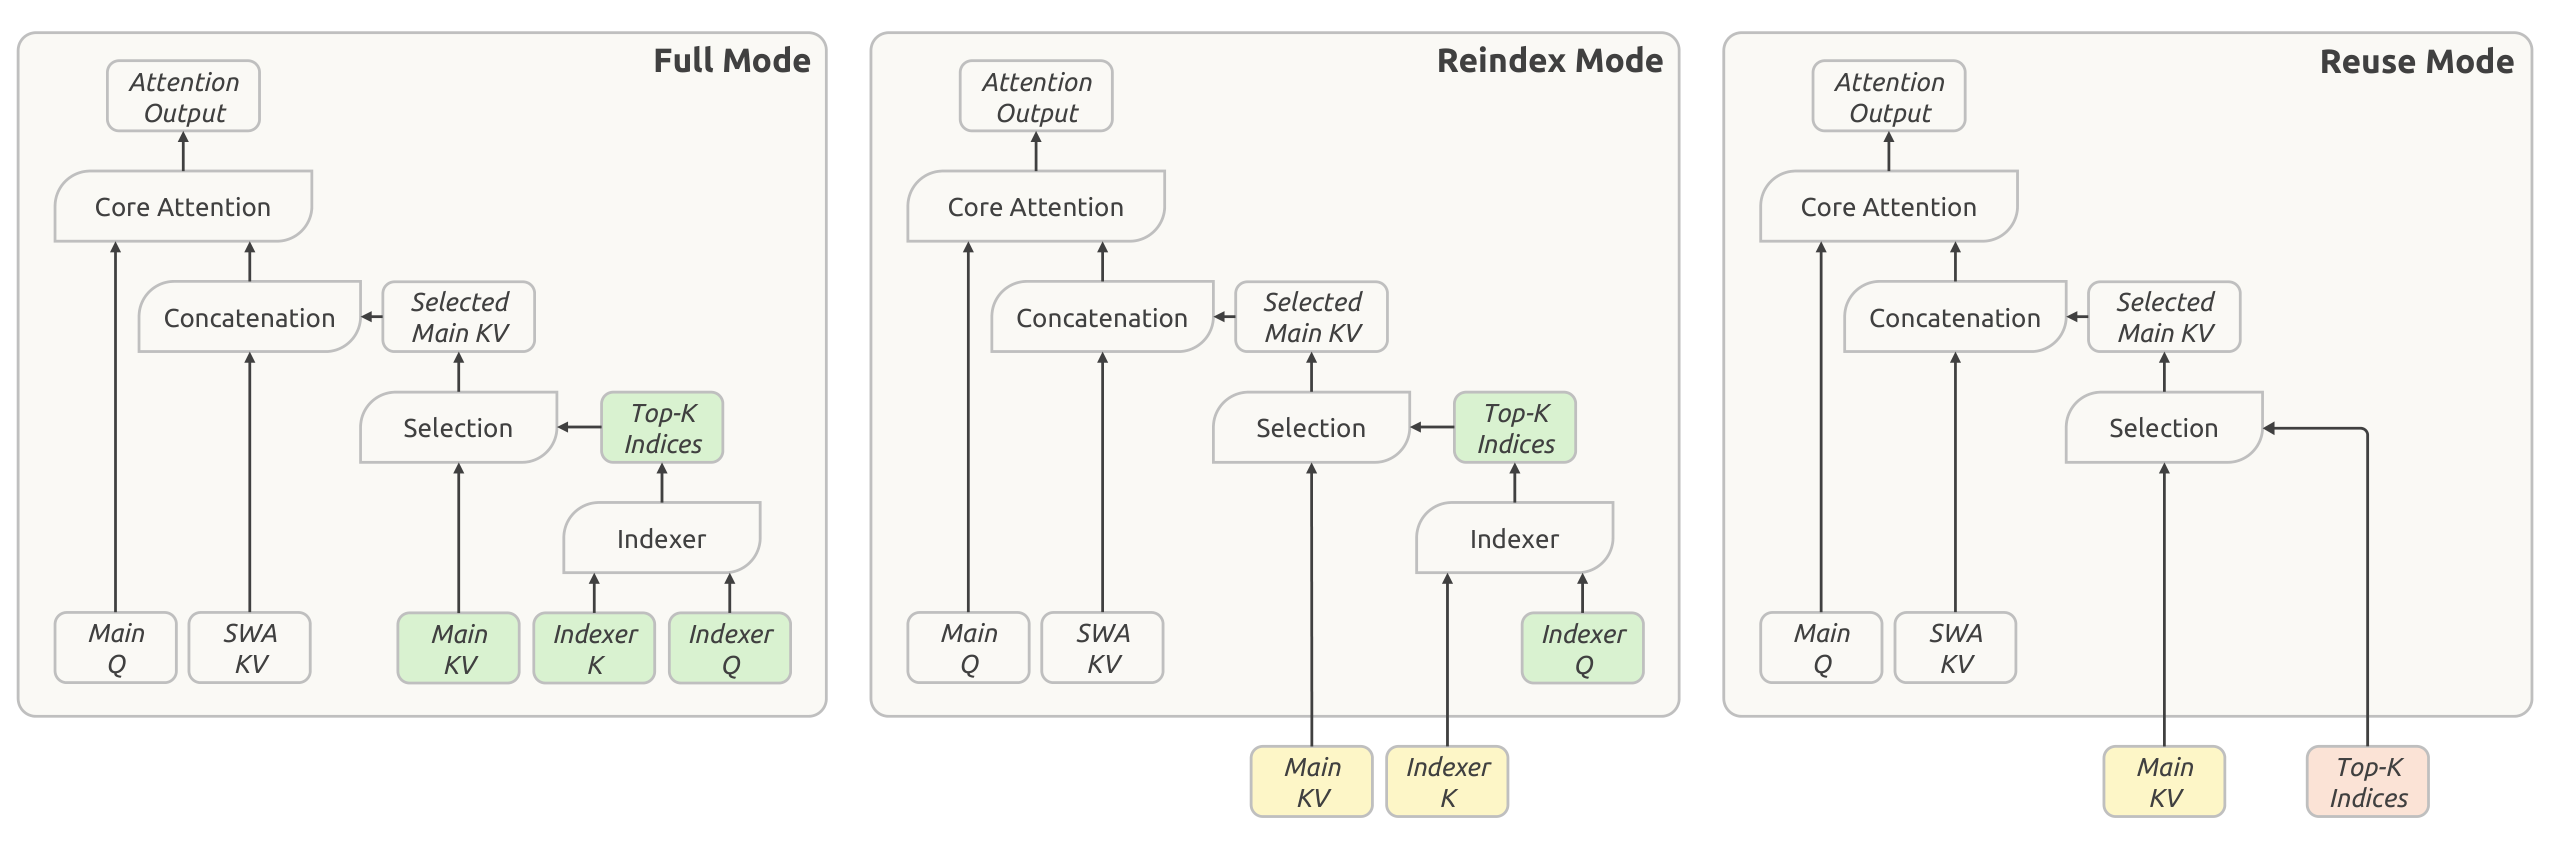
\includegraphics[width=\linewidth]{images_hi/fig04}
\caption{CSA2 的三种运行模式。这些模式在主 KV、索引器 K 和 Top-K 索引的获取方式上有所不同。绿色块表示在当前层中计算的量；黄色块表示从最近的 Full Mode 层复用的主 KV 和索引器 K；红色块表示从最近的生成索引的（Full Mode 或 Reindex Mode）层复用的 Top-K 索引。三种模式均会在当前层计算主 Q 和 SWA KV。}
\label{fig:4}
\end{figure}
\subsubsection{跨层 KV 与索引复用}\label{cross-layer-kv-and-index-reuse}

每个 CSA2 层被静态分配三种模式之一：Full、
Reindex 或 Reuse。在全部三种模式下，该层都计算自己的 query
和 SWA KV，并将其与选定的主 KV 条目一起用于
产生新的注意力输出。各模式的区别在于如何获取主
KV、索引器 K 和 Top-K 索引。图 4 展示了这三种模式。

Full 模式。该层计算自己的主 KV 和索引器 Q，从主
KV 投影出索引器 K，并运行索引器以产生全新的 Top-K
索引。因此它执行完整的 CSA2 计算路径，其组件职责与
DeepSeek-V4 中完整的 CSA2 层








相同。

Reindex 模式。该层复用前面一层中最近可用的主 KV
以及与之对应的索引器 K。索引器计算自己的 query，
对复用的键重新评分，并产生全新的 Top-K
索引。这允许稀疏选择跨层发生变化，
而主 KV 和索引器 K 保持共享。

Reuse 模式。该层复用最近可用的主 KV 和最新
的 Top-K 索引，后者由处于 Full 或 Reindex 模式的前面层
针对该主 KV 计算得出。它使用这一选择执行注意力，
不计算索引器 Q，也不评估索引分数。

共享主 KV 和索引器 K 可减少缓存存储，而复用 Top-K
索引可避免额外的索引器计算。Reindex 模式在保持
缓存共享的同时，允许所选条目跨层发生变化。当
CSA2 与 CED 结合时，被分配为 Full 模式的解码器层会
从第 $(L/2)$ 层的隐藏状态计算自己的全局 KV，即因果编码器的最后一层。Reindex
和 Reuse 模式保持不变。

\subsubsection{层次化稀疏索引器}\label{hierarchical-sparse-indexer}

跨层索引复用减少了索引器评估的次数，但
剩余索引器仍要对完整的因果可见上下文进行评分。
对于极长上下文，这一代价仍是主要的计算
瓶颈。此前的工作通过评分
和剪枝池化块表示，在 token 级索引之前引入了索引器
稀疏性（Xu et al., 2026b）。我们发现，在解码器中，较浅层
索引器的信息自然可以用来限制较深层索引器
所考虑的候选，而无需增加任何额外状态。因此我们引入了
层次化稀疏索引器，它仅用于 CED 的
解码器，以减少解码期间的这种重复评分。对于每个 query，
第一个被分配为 Full 模式的层构建一个候选池，后续
重新索引的各层将其用作搜索域。在候选池大小
固定时，较深层索引器的单 query 代价从关于上下文长度的线性
变为常数。该机制是训练感知的，并在后训练中引入：
候选限制在训练和推理期间以相同方式应用，
因此较深层索引器在与推理时相同的搜索域下被
优化。图 5
说明了这一过程。





第一个 Full 模式层对所有因果可见的主 KV 位置进行评分，
并为其自身注意力产生 Top-K 索引。它还进行
块级候选选择：每个块被赋予其各位置中最大的索引
分数，得分最高的块被选中。然后它将所选块覆盖的位置
收集到一个
比最终 Top-K 集合更大的候选池中。例如，
选择 2,048 个块，每块 8 个位置，可得到 16,384 个候选
位置。该池定义了后续索引器搜索的范围；最终的
Top-K 选择决定每一层读取哪些主 KV 条目。

处于 Reindex 模式的后续层仅对相应 query 的候选位置
进行评分，并在该池内选择自己的 Top-K 条目。处于 Reuse
模式的层不进行新的索引，直接使用针对所复用主 KV 计算出的
最新 Top-K 索引。因此，
候选池在索引层之间共享，而它们最终的
选择可以不同。

在候选池大小固定的情况下，每个后续索引器对每个
query 评分的位置数有界，与上下文
长度无关。第一个 Full 模式层仍会扫描整个因果可见
范围。因此，层次化索引在保留最初的全局扫描的前提下，
降低了后续索引器评估的代价。

\subsection{高效的架构扩展}\label{efficient-architectural-extensions}

\subsubsection{单遍 mHC}\label{single-pass-mhc}

在 DeepSeek-V4 中，我们引入了 mHC（Xie et al., 2026），它在相邻 Transformer
块之间维护 $n$ 条残差流。对每个 token，我们
用 \(X _ { l } \in \mathbb { R } ^ { n \times d }\)
表示这些流，其中 $l$ 是块索引，$d$ 是隐藏维度。这些流
按如下方式更新：

\[
X _ { l + 1 } = B _ { l } X _ { l } + C _ { l } { \mathcal { F } } _ { l } ( A _ { l } X _ { l } ) , \qquad ( A _ { l } , B _ { l } , C _ { l } ) = { \mathcal { H } } ( X _ { l } ) ,\tag{2}
\]

其中
\(A _ { l } \in \mathbb { R } ^ { 1 \times n } , C _ { l } \in \mathbb { R } ^ { n \times 1 }\)
且 \(B _ { l } \in \mathbb { R } ^ { n \times n }\) 是由 $X_l$ 预测的
token 级系数。系数预测器 H 包括
归一化和投影。

理想情况下，两个块之间的残差变换是一个从
\(\left( X _ { l - 1 } , Y _ { l - 1 } \right)\) 到
\(( X _ { l } , \hat { X } _ { l } )\) 的单一映射，其中
\(\hat { X } _ { l } = A _ { l } X _ { l }\) 是当前块的输入，
而
\(Y _ { l - 1 } = \mathcal { F } _ { l - 1 } ( \hat { X } _ { l - 1 } )\)
是上一块的输出。这样的映射需要 $(n + 1)d$ 次读取和
\(( n + 1 ) d\) 次写入，从而对激活内存访问量给出
\(( 2 n + 2 ) d\) 的下界。实际上，DeepSeek-V4 采用公式 (2) 的多遍
实现，包含三个因数据依赖而顺序执行的
内核：

\[
X _ { l } = B _ { l - 1 } X _ { l - 1 } + C _ { l - 1 } Y _ { l - 1 } \qquad { \mathrm { R e s i d u a l ~ u p d a t e , c o n t r a c t i o n ~ o v e r ~ } } n\tag{3}
\]

\[
\left( A _ { l } , B _ { l } , C _ { l } \right) = \mathcal { H } ( X _ { l } )
\]

\[
\mathbf { C o e f f i c i e n t s , c o n t r a c t i o n o v e r } n d\tag{4}
\]

\[
\hat { X } _ { l } = A _ { l } X _ { l }
\]

\[
{ \mathrm { I n p u t m i x i n g } } , { \mathrm { c o n t r a c t i o n o v e r } } n\tag{5}
\]

这三个内核分别读取 $((n + 1)d$、$nd$ 和 $nd$ 个值，
总共写入 \(( n + 1 ) d\)。把
\(\mathcal { F } _ { l } ,\) 中的预归一化算在内，总的激活内存访问量为
\(( 4 n + 4 ) d ,\) , 是下界的两倍。

在 H 中，归一化权重被离线折叠进投影权重，
RMS 除法在投影之后应用。三个阶段中有两个
因此可以共享对残差的一次遍历：
残差更新不需要跨隐藏维度做归约，
因此 \(X _ { l }\) 的每个 tile 都可以被计算出来并立即
用于累加计算 RMS 所需的投影输出和平方和。
输入混合无法融合进这一遍，因为
在对所有隐藏 tile 完成归约之前，
\(A _ { l }\) 不可用。因此它需要对 \(X _ { l } .\) . 进行第二次读取。
这第二遍还可以并入输入预归一化。这种两遍
实现总共需要 $(3n + 2)d$ 次激活读取和写入，
与下界
相比，多了一次对 \(X _ { l }\) 的读取。




因此，我们引入了单遍 mHC：它将输入混合
系数错移一个块，即每个块使用前一个块产生的混合
系数，从而使上述依赖
消失：

\[
X _ { l + 1 } = B _ { l } X _ { l } + C _ { l } \mathcal { F } _ { l } ( A _ { l - 1 } X _ { l } ) , \qquad ( A _ { l } , B _ { l } , C _ { l } ) = \mathcal { H } ( X _ { l } ) .\tag{6}
\]

输入混合现在使用 \(A _ { l - 1 }\) 而不是 \(A _ { l } ,\)，因此它
不再依赖根据 \(X _ { l } .\) . 计算出的系数。
因此，$X_l$ 的每个 tile 可以立即同时用于输入混合
和系数预测，而无须等待完整的归约。
经验上，这种错移带来的性能退化可以忽略不计。

对于预训练，我们保留现有的多内核实现，
因为这种错移只是改变了每个块所应用的混合系数。
对于部署，我们将残差更新、输入混合和
系数预测融合为单一内核 Mega-mHC。该内核
以 $(3n + 2)d$ 次激活读取和写入实现 mHC，
以 \(( 2 n + 2 ) d\) 次激活读取和写入实现单遍 mHC。
Mega-mHC 沿隐藏维度以 tile 为单位处理 \(X _ { l }\)。
每个 tile 都被用来计算混合输入，并累加预测下一个块
的
\(\left( A _ { l } , B _ { l } , C _ { l } \right)\) 所需的量。
该内核还并入输入预归一化和 FP8 转换。这样，
残差被读取一次并写入一次，达到理想映射的 $(n + 1)d$
次读取和 $(n + 1)d$ 次写入，并将我们原有实现的激活内存
访问量减半。

\begin{figure}[htbp]
\centering
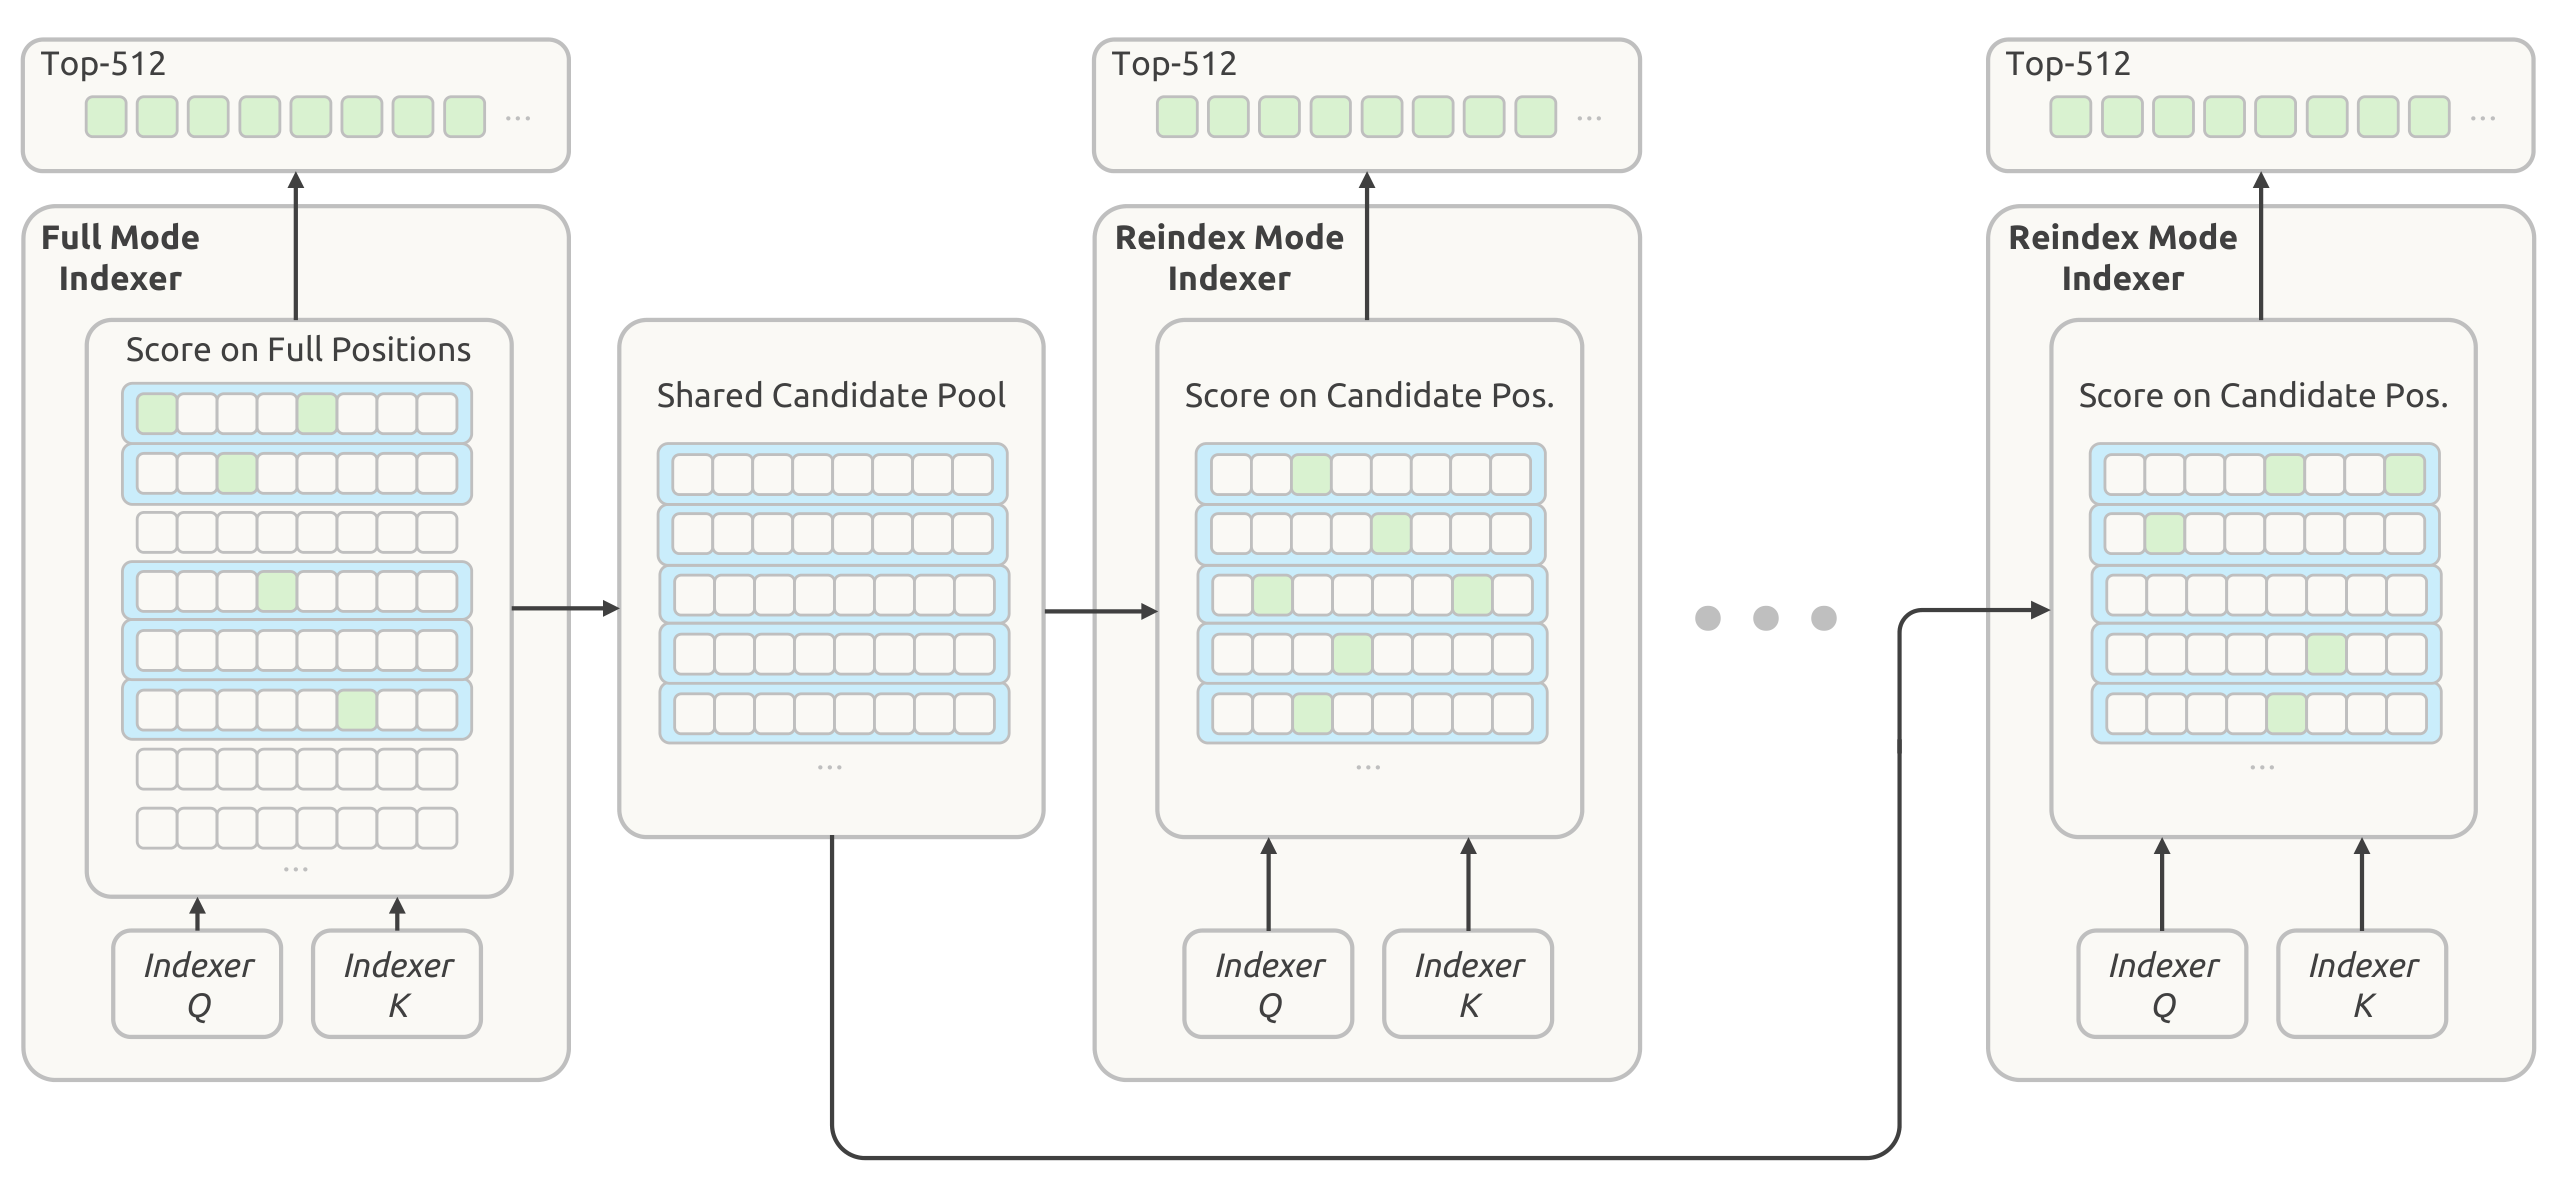
\includegraphics[width=\linewidth]{images_hi/fig05}
\caption{层次化稀疏索引器。每个方块代表一个位置；绿色方块标记被选中的索引，蓝色矩形标记基于其最大索引器得分而选中的块。解码器的第一个 CSA2 层在 Full 模式下选择自己的 Top-512 索引，并从所选块为后续层构建一个共享候选池。处于 Reindex 模式的 CSA2 层随后从该池中选择自己的 Top-512 索引。}
\label{fig:5}
\end{figure}
\subsubsection{Engram}\label{engram}

我们为 DeepSeek-V4.1-Flash 引入 Engram（Cheng et al., 2026c）——这是我们在前期工作中提出的条件记忆模块，用于将记忆与计算解耦。我们沿用原始 Engram 设计——tokenizer 压缩、多哈希头、上下文感知门控与多分支集成——并做了两处修改。第一，我们去掉短因果卷积，因为其性能收益不足以支撑它给推理栈带来的额外复杂度。第二，我们用基于动量的更新配合 Sinkhorn 平衡来优化 Engram embedding，详见第 2.5 节。

我们将 196B Engram 参数均匀分配到两个模块。每个模块使用 \(N\)-gram 阶数 \{2, 3, 4\}，配备 8 个哈希头，每阶的总 embedding 维度为 2048。每个头索引一张约 16M 条目的表，各表大小取互不相同的素数。embedding 表与键/值投影均采用 FP8 精度。两个模块分别置于第 1 层与第 14 层（从 0 开始计数），以平衡各训练流水线阶段的内存占用。推理时，确定性寻址使 embedding 可以通过后台 RDMA 传输从主机内存预取，其中第一个模块的预取与第一个 Transformer 块的计算重叠。Engram 训练与推理的更多实现细节见第 3.1.3 节。

\subsubsection{DSpark}\label{dspark}

我们为 DeepSeek-V4.1-Flash 引入 DSpark（Cheng et al., 2026a），一个将半自回归草稿生成与置信度调度验证相结合的推测解码模块。

草稿模型由三个 Transformer 块组成，滑动注意力窗口为 128 个 token。对其做一次前向即可并行计算五个草稿位置的基础 logits，同时一个轻量级的 Markov 头对草稿 token 之间的依赖关系建模。一个置信度头预测各位置的条件接受概率，用于估计前缀存活概率。调度器将这些估计与实测的引擎吞吐曲线结合，为每个请求动态选择验证长度，目标是在当前系统负载下最大化系统整体的期望 token 吞吐。

与 DeepSeek-V3（DeepSeek-AI, 2024）中在整个预训练期间与主干联合训练的 MTP 模块不同，DSpark 在预训练之后的专门阶段引入。该阶段只训练 DSpark，主干保持冻结。在后训练阶段，我们继续让 DSpark 与主干一同训练，但不将 DSpark 目标的梯度回传到主干。这使 DSpark 与不断演化的策略保持对齐，从而能同时加速在线服务以及 RL 与 OPD 的 rollout 生成。

\subsubsection{FP4 Main KV Cache}\label{fp4-main-kv-cache}

长上下文智能体工作负载需要每请求占用大量 KV 缓存，推高了服务成本。DeepSeek-V4 已对 FP4 索引器查询与键采用量化感知训练（QAT）（Jacob et al., 2018），以加速索引计算并缩减索引器缓存规模。我们采用 OCP 标准的 MXFP4 格式（Rouhani et al., 2023），以尽可能多地支持硬件平台，尽管在我们的实验中其他格式精度更高。现在我们进一步将 QAT 扩展到主 KV 缓存，此时 FP4 的作用是压缩存储而非加速矩阵乘法。在注意力计算前对缓存值做反量化，使我们能够使用精度更高的格式，而无需该格式具备原生矩阵乘法支持，从而保持跨硬件平台的兼容性。

在评估过的约 4-bit 格式中，我们选择 E2M1，每 16 个通道配一个 E4M3 scale，沿用 NVFP4（Alvarez et al., 2025）但省略其第二级全局 scale，以在精度与简洁性之间取得平衡。省略该 scale 后，主 KV 缓存仍有充足的动态范围：该格式可表示的最大幅值为 448 \(\times\) 6 = 2688，远高于缓存的幅值上界。在 DeepSeek-V4.1-Flash 中，训练得到的 RMSNorm 权重幅值最大约为 1。经过 RMS 归一化后，512 通道 KV latent 的 L2 范数最多约为 512。RoPE 保持该范数不变，因此旋转后各通道绝对值的最大值同样被限制在约 512 \(\approx\) 22.6 以内。此外，训练期间观测到的最大幅值约为 10。因此，省略全局 scale 不会带来可测量的精度下降，并简化了缓存布局。

为在 DeepSeek-V4.1-Flash 中启用 FP4 主 KV 缓存存储，我们在后训练阶段引入 QAT。非 RoPE 分量与 RoPE 分量使用相同的量化格式。我们在 RoPE 之后对缓存做量化：实验表明在 RoPE 之前量化只能带来微弱的精度提升，却会在解码时引入额外开销。由于 SWA KV 缓存对量化较为敏感，我们对其保留 FP8。与 DeepSeek-V4 的 FP8 主 KV 缓存相比，该格式使存储占用近乎减半，无论是在 HBM 中还是卸载到 SSD 时。
\subsection{Optimization}\label{optimization}

在 DeepSeek-V4 所用优化配置的基础上，我们做了一些新的修改，以更好地契合架构设计。

第一，我们采用逐头 Muon（head-wise Muon），即在应用 Muon 更新前按头切分 Query 权重。这里我们简要讨论该设计的动机。把 Muon 视为一种预条件梯度下降，原始 Muon 对所有头使用同一个预条件子，而逐头 Muon 为不同头提供不同的预条件子。该设计能更好地处理注意力头之间的异质性（Zhang et al., 2024; Zhang, 2026, Section 3）。因此我们观察到逐头 Muon 优于原始 Muon。逐头 Muon 的经验优势也在 GLM 5（Zeng et al., 2026）和 Kimi-K3（Team et al., 2026a）中得到验证。

第二，将 Adam 用于新引入的 Engram 参数会大幅增加优化器状态的内存占用。为降低训练内存开销，我们改为用基于动量的更新配合 Sinkhorn 平衡来优化 Engram embedding 表、token embedding 与预测头。Sinkhorn 平衡此前已被用于 SinkGD（Scetbon et al., 2025）中线性层的权重矩阵；这里我们将其推广到这些大型参数矩阵。与 Muon 类似，该方法只需一个动量缓冲区，同时在经验上优于 Adam。

基础配置。我们对归一化层权重以及其他非矩阵参数（包括偏置与缩放因子）保留 AdamW（Loshchilov and Hutter, 2019）。我们对语言模型主干中线性变换的权重矩阵、Engram 投影层以及视觉-语言投影器使用 Muon（Jordan et al., 2024）。对 Query 与 Key 权重使用逐头 Muon。我们对 Muon 应用解耦权重衰减与 Nesterov 动量（Nesterov, 1983; Liu et al., 2025）；归一化层权重同样受权重衰减作用，而偏置与缩放因子不受。Sinkhorn 平衡更新也使用 Nesterov 动量，但不应用权重衰减。预训练期间，我们保持视觉编码器冻结直至学习率衰减阶段，而其最后的归一化层与视觉-语言投影器始终可训练。在学习率衰减开始时，我们解冻视觉编码器，并以更小的学习率与 LLM 联合优化。

Engram / Embedding / 预测头的 Sinkhorn 平衡更新。完整流程见算法 1。整体上它沿用与 Muon 相同的工作流，只是用 Sinkhorn 平衡替代 Newton--Schulz 正交化。我们用 \(m ,\) 表示较大的矩阵维度，对应 embedding 表与预测头的词表规模，并用 \(n\) 表示隐藏维度。

给定 Nesterov 动量更新 \(\widehat { G } _ { t } ,\) ，Sinkhorn 平衡寻找对角缩放矩阵 \(D _ { r }\) 与 \(D _ { c }\) 使得

\[
\Delta _ { t } = \sqrt { n } U ^ { ( K ) } = \sqrt { n } D _ { r } \widehat { G } _ { t } D _ { c } , \qquad \frac { 1 } { n } \sum _ { j = 1 } ^ { n } ( \Delta _ { t } ) _ { i j } ^ { 2 } \approx 1 , \qquad \frac { 1 } { m } \sum _ { i = 1 } ^ { m } ( \Delta _ { t } ) _ { i j } ^ { 2 } \approx 1 ,\tag{7}
\]

由此，该过程近似地使更新矩阵的行向与列向 RMS 相等。这里一行对应一个 token 索引或 n-gram 标识，一列编码一个隐藏特征。Sinkhorn 平衡利用这种 token--特征结构，同时沿行与列做归一化。为保证数值稳定性，满足 \(\rho _ { i } \leqslant \tau \bar { \rho }\) 的行会被掩蔽。因子 \(\sqrt { n }\) 将单位行 \(\ell _ { 2 }\) 范数转换为单位行向 RMS。另外，我们按 \(\widetilde { \eta _ { t } } = \gamma \eta _ { t }\) 调整有效学习率，以匹配 Adam 的更新幅度。我们取 \(\gamma = 0 . 1 8 ,\) 接近 Moonlight（Liu et al., 2025）中使用的 0.2。

更广泛地说，Sinkhorn 平衡与那些利用矩阵或张量轴结构的优化器密切相关（Shazeer and Stern, 2018; Zhang et al., 2025a; Wen et al., 2025; Glentis et al., 2025; Deng et al., 2026; Yuan et al., 2026; Xu et al., 2026a）。例如，Adafactor（Shazeer and
算法 1 带 Sinkhorn 平衡的动量更新 输入：权重
\(W _ { t } \ \in \ \mathbb { R } ^ { m \times n }\) , 梯度
\(G _ { t } ,\) 动量 \(M _ { t - 1 } ,\) ，动量系数
\(\beta ,\) 基础学习率 \(\eta _ { t } ,\) 学习率修正 $\gamma$，数值常数 $\epsilon$ 与 \(\tau ,\) 以及奇数次的
归一化步数 \(K\) 1:
\(M _ { t } \gets \beta M _ { t - 1 } + ( 1 - \beta ) G _ { t }\) 2:
\(\widehat { G } _ { t } \gets \beta M _ { t } + ( 1 - \beta ) G _ { t }\)
$\triangleleft$ Nesterov 动量 3:
\(\rho _ { i } \gets \| \widehat { G } _ { t , i , : } \| _ { 2 }\) and
\(\textstyle { \bar { \rho } } \gets { \frac { 1 } { m } } \sum _ { i = 1 } ^ { m } \rho _ { i }\)
4: \(U ^ { ( 0 ) } \gets \widehat { G } _ { t }\) 5: 置
\(U _ { i , : } ^ { ( 0 ) } \gets 0\) 若
\(\rho _ { i } \leqslant \tau \bar { \rho }\) $\triangleleft$ 掩蔽近零行 6:
对 \(k ^ { \stackrel { \prime } { = } 1 , \ldots , K }\) 执行 7: 若 $k$ 为奇数则 8: 对所有 \(i = 1 , \ldots , m\) 执行 9:
\(U _ { i , : } ^ { ( k ) } \gets \dot { U } _ { i , : } ^ { ( k - 1 ) } / ( \| U _ { i , : } ^ { ( k - 1 ) } \| _ { 2 } + \varepsilon )\)
10: end for 11: 否则 12: 对所有 \(j = 1 , \dotsc , n\) do 13:
\(U _ { : , j } ^ { ( k ) ^ { \prime } } \gets \dot { U } _ { : , j } ^ { ( k - 1 ) } / ( \lVert U _ { : , j } ^ { ( k - 1 ) } \rVert _ { 2 } + \varepsilon )\)
14: end for 15: end if 16: end for 17:
\(\Delta _ { t } \gets \sqrt { n } U ^ { ( K ) }\) $\triangleleft$ 将单位行
\(\ell _ { 2 }\) 范数转换为单位行 RMS 18:
\(\widetilde { \eta _ { t } }  \gamma \eta _ { t }\) $\triangleleft$ 匹配
的更新幅度 19:
\(W _ { t + 1 } \gets W _ { t } - \widetilde { \eta _ { t } } \Delta _ { t }\)

Stern, 2018）以另一种方式做行向与列向归一化，而 Adammini（Zhang et al., 2025a）对 embedding 表与预测头采用另一种行向归一化。这些归一化策略可能在优化性能与通信开销上存在差异。更细致的研究我们留作未来方向。
\section{通用基础设施}\label{general-infrastructures}

\subsection{Training Infrastructure}\label{training-infrastructure}

\subsubsection{Multimodal Training Infrastructure}\label{multimodal-training-infrastructure}

对比学习中的通信-计算重叠。视觉编码器首先以对比目标进行优化，随后再用生成式下一 token 预测损失进行微调。在对比阶段，损失是在一整批文本-视觉配对样本上计算的，因此两种模态的特征都必须跨数据并行 rank 做 all-gather，产生可观的通信量。由于文本特征的梯度只依赖于汇聚得到的视觉特征，并且对称地，视觉特征的梯度也只依赖于汇聚得到的文本特征，因此每个 all-gather 都可以与前向或反向传播重叠，而不是拖住整条流水线：

\[
\begin{array} { r l } { \mathrm { F o r w a r d } ( V ) ~ \to ~ \left( \mathrm { F o r w a r d } ( T ) ~ \lVert ~ \mathrm { A l l G a t h e r } ( V ) \right) ~ \to ~ \nabla _ { \mathrm { T e x t } } } & { } \\ { \to ~ \left( \mathrm { B a c k w a r d } ( T ) ~ \lVert ~ \mathrm { A l l G a t h e r } ( T ) \right) ~ \to ~ \nabla _ { \mathrm { V i s i o n } } ~ \to ~ \mathrm { B a c k w a r d } ( V ) , } \end{array}
\]

其中 $V$ 和 $T$ 分别表示视觉与文本特征，
\(\left( A \parallel C \right)\) 表示计算 $A$ 与通信 \(C\) 的重叠，$\nabla$ 表示梯度计算。在这种调度下，视觉特征在文本前向传播期间被汇聚，文本特征在文本反向传播期间被汇聚，从而两个 all-gather 都完全隐藏在有效计算之后。



端到端并行。为处理视觉编码器与 LLM 之间的模型和数据异构性（Zhang et al., 2025b），我们采用了近期训练系统中使用的解耦编码器设计（Team et al., 2025, 2026b）。视觉编码器在 LLM 参数树之外进行复制，每个训练步骤被划分为三个阶段：视觉编码器前向、LLM 前向/反向，以及视觉编码器反向。这种分离避免了视觉编码器与 LLM 计算之间的相互干扰。负载均衡的视觉处理被限制在第一和最后一个阶段，而 LLM 阶段不包含视觉计算，从而保留了纯文本训练的并行策略。

长序列多模态训练优化。DeepSeek-V4.1-Flash 在最长包含一百万个 token 的序列上训练，其中相当一部分训练发生在预训练和后训练阶段的超长序列上。在这些序列长度下，多模态样本会带来严重的 I/O、CPU 和内存瓶颈。

• 均衡图像分片。在预训练期间，一条超长的、图像密集的序列在加载时就可能耗尽单个主机的
\(\mathrm { I } / \mathrm { O } ,\) CPU 和内存，因此每条序列中的图像都以负载均衡的方式分片到各 CP rank 上，并且每张图像只加载一次。由于图像只读取一次，只要满足以下条件，加载即可被计算完全掩盖：

\[
\frac { N \times \rho } { B _ { \mathrm { I O } } } < \frac { N \times C } { B _ { \mathrm { G P U } } } \quad \Longleftrightarrow \quad \rho < \frac { B _ { \mathrm { I O } } } { B _ { \mathrm { G P U } } } C ,
\]

其中 $N$ 是 token 数，$\rho$ 是每个 token 的原始字节数，$C$ 是每个 token 的计算量，而 \(B _ { \mathrm { I O } }\)
\(B _ { \mathrm { G P U } }\) 分别是文件系统与 GPU 的带宽。由于 $N$ 会被约去，该判据只涉及每 token 的量（$\rho$ 和 $C$），
与序列长度和集群规模无关；$\rho$ 由视觉模块的配置决定（例如分辨率上限或空间降采样）。因此，存储吞吐只在每 token 计算量较低的小模型上成为瓶颈，例如在消融实验中，而生产级模型仍保持计算受限。

• 增量式图像传输。除上述均衡分片外，强化学习（reinforcement-learning）rollout 只将图像增量式地传输到推理引擎，并把引擎 CPU 侧的解码与预处理输出缓存在分布式文件系统上，以便在多次 rollout 以及后续训练中复用。

\subsubsection{面向 CSA2 的注意力共享训练}\label{attention-sharing-trainingfor-csa2}

在第 2.3 节中，我们介绍了 CSA2——一种具有三种模式的注意力共享方法，其中某些模式涉及跨多个层共享主 KV、索引器 K 和 Top-K 索引中的一个或多个。在大规模分布式训练中支持 CSA2，除了注意力计算本身之外，还需要额外的协调。特别是，共享注意力组件的层可能被放置在不同的流水线阶段，这使得直接复用模块与常规的阶段局部执行不兼容。因此，我们采用了多种设计来支持 CSA2 训练。

影子索引器通过在每个参与阶段放置一个轻量的可执行副本，同时为共享参数保留单一逻辑所有者，来解决上述问题。所有者仍负责优化和检查点保存，而参数同步与梯度聚合使各影子副本在整个训练过程中保持一致。这一设计保留了原始模型语义，同时无须让流水线调度器把共享层当作特殊的执行单元。



流水线载荷扩展：当源层与消费层跨越流水线边界时，为其下游消费者提供所需的中间表示和稀疏路由信息。这些状态被并入现有的点对点通信路径，并与上下文并行保持一致地分区，从而在维持相应梯度流的同时避免不必要的复制。

微批级共享状态管理跟踪与并发活跃的流水线微批相关联的状态，并协调这些状态在前向执行、激活重计算和反向传播中的生命周期。共享状态会一直保留到其最终消费者完成之后才被及时释放，以限制额外的内存开销。同一套运行时抽象还处理阶段放置与源-消费层关系，使注意力实现无须依赖物理流水线布局即可访问共享状态。

结合对优化器、检查点保存、预热和计算图追踪流程的轻量适配，这些机制使 CSA2 能够在既有分布式训练接口和流水线调度下透明地运行。

\subsubsection{Engram}\label{engram-1}

Engram 嵌入表按行分区，分布到 engram 并行大小的专用进程组上。组大小控制着每设备内存占用与嵌入查找通信范围之间的权衡。优化器状态进一步被分片到每个表分区的副本上。Engram 查找索引仅取决于输入的 token 序列。因此，在每个流水线阶段开始为当前训练步骤处理微批之前，就会为整个本地批次发起嵌入预取，从而最大限度地减少对流水线执行的干扰。嵌入梯度在反向传播期间被缓冲，并在骨干网络反向传播之后返回给其所属的 rank。为了实现与多模态训练的高效集成，嵌入预取和梯度传输被调度为与视觉编码器的前向和反向计算重叠。嵌入以 FP8 格式存储和读取，取回的值和缩放因子直接传递给后续的 GEMM。对于 Engram 表更新，Sinkhorn 归一化会在各迭代之间维护行和列的缩放向量，以避免重复写入完整的归一化矩阵。行归一化与部分列统计的累加被融合到单个 kernel 中，以进一步减少内存访问量。在 RL rollout 期间，Engram 嵌入表常驻 GPU 内存。这种放置方式降低了主机内存压力，并有助于避免由主机内存碎片化导致的内存不足故障。

\subsection{推理系统}\label{inference-system}

DeepSeek-V4.1-Flash 将推理效率作为首要考量来设计。尽管其架构在概念上较为复杂，但最终形成的推理 kernel 流程却异常简洁。通过合理的 kernel 融合，我们将这些复杂运算封装进少数几个融合 kernel 中，使硬件资源在这些 kernel 内部保持完全流水化——包括 FlashMLA（Li and Liu, 2025）中的 fused-RoPE-attention-RoPE-cast kernel、DeepGEMM（Zhao et al., 2025）中的 Mega-Gate、Mega-mHC 和 Mega-MoE kernel、TileKernels（Wang et al., 2026a）中的各 kernel，以及 DeepSelect（Qian et al., 2026）中的 TopK kernel。因此，绝大多数



Transformer 层——即 CSA2 以 Reuse 模式运行的层——在预填充阶段只需 15 个 kernel、在解码阶段只需 11 个 kernel 即可执行，从而同时实现高吞吐与低延迟推理。

在部署层面，我们采用编码器-预填充-解码（EPD）解耦架构，使视觉编码、预填充和解码能够独立扩展并重叠执行。
\subsubsection{持久化 KV 缓存管理}\label{persistent-kv-cache-management}

在相同负载下，V4.1 将持久化 KV 缓存的占用降至 V4 的 \(1 / 8\)。这一缩减由相乘的两个因素共同实现：持久化 KV 缓存不再存储 SWA KV，使其规模几乎减半；缓存中保留的全局 KV 又经由架构与精度优化被进一步压缩至 V4 的 1/4。

在 V4 部署中，SWA KV 几乎占去持久化 KV 缓存容量的一半。在此缓存中，全局 KV 与 SWA KV 由 LRU 淘汰策略独立管理。全局 KV 被完整存储，命中后即复用完整前缀。相比之下，SWA KV 被缓存于两个特定位置——提示末尾与输出末尾——以支持重生成与多轮会话；命中时计算可从该缓存位置继续。为维持较高的命中率，我们在 SSD 上配置了足够大的持久化 KV 缓存，使典型工作负载下两类 KV 均能常驻超过 72 小时。尽管仅在指定位置保留 \(n _ { \mathrm { W i n } }\) 个 KV 条目，未压缩的 SWA KV 缓存仍带来可观的存储开销，尤其是在轮次较短的多轮对话中。

持久化存储 SWA KV 既代价高昂又收效甚微，因为其访问模式与持久化 KV 缓存的长效保留策略不匹配。与表现出长尾复用的全局 KV 不同，SWA KV 只在活动会话内部一个狭窄、以分钟计的窗口内被复用，一旦会话结束或下一轮开始即告失效。V4 技术报告提出了 Zero SWA Caching，通过重算缺失的 SWA KV 来规避存储开销。然而，精确恢复需要对 \(L \times n _ { \mathrm { w i n } }\) 个 token 执行一次完整的前向传播，这一成本在生产部署中被证明是不可承受的。

因此，V4.1 对持久化 KV 缓存的管理方式修订如下：

\begin{enumerate}
\def\labelenumi{\arabic{enumi}.}
\item
  SWA KV 不再缓存于持久化 KV 缓存，而是存入由每台机器 10\% 的主机 DRAM 划拨形成的分布式内存池。尽管该池在总容量上远小得多，但其较短的 TTL（仅有几分钟）允许过期条目被立即回收用于新会话；在真实工作负载下，这种高周转率足以服务绝大多数并发活动会话。全局 KV 仍保留在持久化 KV 缓存中，保证其生命周期至少为 72 小时。
\item
  逐出 SWA KV 不可避免地会造成未命中，而一种轻量级兜底机制——编码器 SWA 有界回放（详见 3.2.2 节）——使这类未命中仍可承受。对于那些命中全局 KV 但未命中 SWA KV 的必然却罕见的请求，它只对 \(n _ { \mathrm { w i n } }\) 个 token 进行重算，而非执行一次完整的 \(L \times n _ { \mathrm { w i n } }\) token 前向传播，从而恢复缺失状态。这种有界回放是整套设计的基础：它将灾难性的未命中转化为优雅而廉价的性能降级，进而为移除持久化 KV 缓存中的 SWA KV 提供了依据。
\end{enumerate}



\subsubsection{SWA 有界回放}\label{swa-bounded-replay}

由于 SWA 依赖关系在各层间累积，对 $L$ 层 SWA KV 的精确重建需要回放 \(L \times n _ { \mathrm { w i n } }\) 个 token。SWA 有界回放只回放最近的 \(n _ { \mathrm { { w i n } } }\) 个 token，并将 SWA 截断至回放片段，从而接受近似状态：对于从位置 $s$ 开始的回放，位置 $i$ 的查询会注意 $[\max(s, i - W + 1),\ i]$ 范围内的 SWA 键。

编码器 SWA 有界回放。编码器 SWA 有界回放使前缀缓存只依赖全局 KV，从而可将 SWA KV 从持久化 KV 缓存中移除。

当编码器 SWA KV 缺失时，我们回放已缓存前缀的最后 \(n _ { \mathrm { W i n } }\) 个 token，并将其与未缓存的后缀一同处理。被回放的 token 仅重新生成 SWA KV，并复用已缓存的全局 KV，既不重算也不覆盖；而未缓存的后缀则同时生成全局 KV 与 SWA KV。

按设计，回放得到的前缀状态是近似的，因此为未缓存后缀计算出的全局 KV 与 SWA KV 依赖于缓存命中位置，在不同位置之间并不数学一致。令人鼓舞的是，我们的实验证据表明，这种有界回放策略对响应质量的损害可以忽略不计。

解码器 SWA 有界回放。解码器 SWA 有界回放将解码器前向传播限定在 \(n _ { \mathrm { w i n } }\) 个 token 之内，使预填充总计算量几乎减半。

在 CED 下，解码器全局 KV 由编码器最终隐藏状态投影而来。在编码器处结束预填充的唯一障碍是解码器 SWA KV，它由每个解码器层自身的隐藏状态生成，并为最初的若干解码步骤所需。由于我们从不缓存解码器 SWA KV，精确重建它需要让 \(\frac { L } { 2 }\) 个解码器层处理最后 \(\frac { L } { 2 } \times n _ { \mathrm { w i n } }\) 个提示 token，当较短的未缓存后缀紧跟较长的已缓存前缀时，这一过程代价高昂。因此，我们也把有界回放策略应用于该场景：在每次预填充时，我们回放提示的最后 \(n _ { \mathrm { W i n } }\) 个 token，在相同的 SWA 截断下将其编码器输出经过解码器各层，并把由此得到的解码器 SWA KV 仅用于解码，而不用作前缀缓存。

按设计，重建出的解码器 SWA KV 与完整解码器前向传播所得在数学上并不等价。同时我们发现，这一策略对响应质量仅有可忽略的影响。为更加稳妥，我们还在后训练阶段模拟同样的回放，实现面向训练的适配。

\section{预训练}\label{pre-training}

\subsection{数据构建}\label{data-construction}

文本数据策展。为追求更高的智能水平，我们不再局限于小规模数据实验所反映的通用、样本级质量，而是更关注那些能带来独特信息增益的多元语料之间的整体互动。我们采用更系统、更规范的数据构建流水线，以提升数据质量并优化数据配比。具体而言，在更全面的评测基础上，我们精心设计了一个横跨模型参数与训练数据的缩放阶梯（scaling ladder），用以指导大规模训练。我们过滤掉信息增益有限的模型生成内容，包括能力较弱的模型产生的输出以及低质量的机器翻译文本。我们认为此类内容属于隐式重复，因为它在很大程度上只是对既有信息的改述，并可能在长期训练中产生负面影响。我们还探索了模型在环（model-in-the-loop）的数据迭代方法，作为未来大规模合成数据的基础。此外，我们引入更多领域专家，构建细粒度的数据质量评测维度。与前一版本相比，新语料纳入了更多来自新发布的开源仓库、代码提交、代码库与新兴框架的近期代码，从而覆盖更广泛的编程语言，更好地反映当代真实世界的软件工程场景。



多模态数据策展。我们的多模态预训练数据集主要包括三类数据：图文对、交错图文数据与领域专属数据。鉴于原始网页数据天然蕴含丰富的多模态知识，我们没有进行大规模数据合成，而是优先对数据进行清洗并以其原生形式加以利用，以便在预训练阶段实现最直接、可扩展的视觉知识压缩。在最初的数据采集过程中，我们发现抓取系统过度偏向以文本为中心的网页内容，因此我们以 Common Crawl 为源对其重新引导，以提升对多模态来源的覆盖。对于图文对，我们从网页中提取图像及其关联的 alt 文本，通过图文相关性阈值进行过滤，并基于图像语义进行去重。对于交错数据，我们主要从网页与 PDF 构建这一子集。处理大规模多模态语料通常比处理纯文本语料产生更高的 CPU 与磁盘存储开销，这促使我们将交错数据的构建组织为逐渐增耗的阶段。在图像检索之前，我们先施加启发式与统计过滤、去重及质量模型，以筛选出高价值的文档。通过筛选的文档随后被组装成交错图文序列，此时再次以图像感知的方式进行过滤与去重。最后，我们使用 SmolVLM（Marafioti 等人，2025）对图文内容进行严格的质量评分，从而提取高质量的交错数据。该过程中被过滤掉的文档有一部分经由筛选与重组，被回收为额外的图文对。为弥补从网络采集数据的固有局限，我们还纳入领域专属数据集，以增强模型在细粒度视觉感知（例如视觉定位与指认）、光学字符识别（OCR）以及长尾知识获取方面的能力。我们还收集了大量图像—代码对与计算机使用轨迹，以提升多模态智能体理解能力。

数据整合与去重。由于我们的纯文本数据与多模态数据经由不同的流水线处理，我们把最终训练语料构建为两类数据源的并集。对于重叠样本，我们用多模态版本替换纯文本版本，并采用两种配置中较大的轮数。完成替换后，最终语料的纯文本与多模态数据按 7:1 的 token 比例构成。我们通过联合预取与分配训练样本，将预训练与上下文扩展期间的样本重叠降至最低。超长文档在混料之前被确定性预切分，以确保训练 token 在数据分片与训练步骤之间均匀分布。我们还进一步增强了最佳适配打包（best-fit packing）算法，将填充率降至至多 10−4。
\subsection{预训练设置}\label{pre-training-setups}

\subsubsection{模型设置}\label{model-setups}

我们将 Transformer 的层数设为 40，隐藏维度 $d$ 设为 5120。我们采用因果编码器-解码器（Causal Encoder-Decoder）架构，其中编码器 20 层、解码器 20 层。对于前两层，我们使用纯滑动窗口注意力。其余 18 个编码器层使用压缩率 \(m = 2\) 的 CSA2。这些层被划分为三组，每组六层、配置完全相同。每一组中，第一层以 Full 模式运行，其余五层以 Reuse 模式运行。20 个解码器层使用压缩率 \(m = 1\) 的 CSA2，划分为五组，每组四层。在第一组中，第一层以 Full 模式运行，其余三层以 Reuse 模式运行。其余四组共享相同的配置：第一层以 Reindex 模式运行，其余三层以 Reuse 模式运行。对于所有 CSA2 层，我们将索引器查询头数设为 32，索引器头维度设为 128，稀疏注意力（即 attention top-k）选取的 KV 条目数设为 512。我们将查询头数设为 64，头维度设为 512，查询压缩维度设为 1280。对于分层稀疏索引器（Hierarchical Sparse Indexer），我们最多选择 2,048 个块、每块 8 个位置，总共最多产生 16,384 个候选位置。输出投影组数设为 8，每个中间注意力输出的维度设为 1024。对于滑动窗口注意力的附加分支，窗口大小 \(n _ { \mathrm { W i n } }\) 设为 128。我们在所有 Transformer 块中采用 MoE 层，使用带钳制（clamping）的 SwiGLU 激活函数（OpenAI, 2025），阈值设为 10。每个 MoE 层包含 1 个共享专家和 384 个路由专家，每个专家的中间隐藏维度为 2304。在路由专家中，每个 token 激活其中 6 个。对于 mHC，扩展因子设为 4，Sinkhorn-Knopp 迭代次数设为 20。对于视觉编码器，我们将其层数设为 32，隐藏维度设为 1024，注意力头数设为 16，图像 patch 大小设为 14。视觉 MLP 投影器有 2 层，隐藏维度为 5120。在此配置下，DeepSeek-V4.1-Flash 包含 552B 主干参数，prefill 阶段每个 token 激活 8B，decode 阶段激活 16B。



\subsubsection{训练设置}\label{training-setups}

对于线性变换的参数，我们使用 Muon 优化器（Jordan et al., 2024; Liu et al., 2025）；对于所有 RMSNorm 模块及其他非矩阵参数的权重，使用 AdamW 优化器（Loshchilov and Hutter, 2019）；对于所有 embedding 和预测头，使用 Sinkhorn 平衡（Sinkhorn-balanced）更新。对于 AdamW，我们将其超参数设为 \(\beta _ { 1 } = 0 . 9 , \beta _ { 2 } = 0 . 9 5 , \varepsilon = 1 0 ^ { - 2 0 }\), 以及 weight\_decay = 0.1。对于 Muon，我们将动量设为 0.95、权重衰减设为 0.1，并将每个更新矩阵的 RMS 重标定为 0.18，以便复用 AdamW 的学习率。对于 Sinkhorn 平衡更新，我们使用与 Muon 相同的动量系数和学习率修正因子，并设 \(K = 1 1 , \tau = 1 0 ^ { - 3 } , \varepsilon = 1 0 ^ { - 2 0 }\)。参照（Cheng et al., 2026b），Engram 的学习率按 5$\times$ 缩放。我们在 45T token 的多模态数据上训练 DeepSeek-V4.1-Flash，全程无训练不稳。整个训练过程中，批次大小固定为 100.6M 个 token。学习率在前 2000 步线性预热，随后保持 \(2 . 6 \times 1 0 ^ { - 4 }\) 直到 28T token。在 28T 到 40T token 之间，我们按余弦调度将学习率衰减至 \(2 . 6 \times 1 0 ^ { - 5 }\)。从 40T 到 45T token，学习率保持在该值。我们从零开始训练模型，在序列长度 64K 下使用稀疏注意力，并在 34T token 处将序列长度扩展到 1M。对于无辅助损失（auxiliary-loss-free）的负载均衡，我们将图像和文本 token 的偏置更新速度均设为 0.001，同时保留一个损失权重为 0.0001 的小型序列级均衡损失，以避免单个序列内出现极端不均衡。与 DeepSeek-V4 类似，我们在预训练期间采用样本级注意力掩码。

视觉编码器训练。我们的 DeepSeek-ViT 在与语言主干集成之前，会经过一个单独的训练阶段。训练流程包含两个阶段：对比预训练和自回归微调。在对比预训练阶段，我们使用 SigLIP（Zhai et al., 2023）引入的 sigmoid 对比损失，在约 47B 条来自 alt-text 数据的图像-文本对上优化模型。为了在如此大规模的数据集上高效学习视觉表征，我们通过按比例缩小较大的图像并保持其宽高比，将最大输入分辨率限制在 224 $\times$ 224 像素。虽然在此阶段使用更高分辨率会带来可观收益，但实验结果表明，这些收益对最终模型的贡献很小。由于后续自回归阶段专门处理高分辨率外推，在对比预训练阶段提高分辨率会显著增加计算开销，却不会带来多大的整体改善。在自回归微调阶段，我们将视觉编码器连接到 4B MoE LLM，在涵盖图像描述、alt text、图表和 OCR 等数据集的 236B token 上进行训练，使用下一 token 预测目标。该阶段旨在增强编码器对细粒度视觉特征建模的能力。因此，我们通过按比例缩放超出范围的图像，将输入分辨率约束在 544 $\times$ 544 到 1344 $\times$ 1344 像素之间。此阶段结束后，我们丢弃 LLM，仅保留优化后的视觉编码器用于后续预训练流程，并继续采用相同的输入分辨率策略。



\subsection{评测}\label{evaluations}

\subsubsection{评测基准}\label{evaluation-benchmarks}

我们将 DeepSeek-V4.1-Flash-Base 与其前代模型 DeepSeek-V4-Flash-Base 和 DeepSeek-V4-Pro-Base 进行对比。我们报告的基准涵盖五个关键维度：世界知识、语言理解与推理、代码与数学、长上下文，以及多模态能力。

世界知识基准包括 AGIEval（Zhong et al., 2023）、MMLU-Pro（Wang et al., 2024b）、C-Eval（Huang et al., 2023）、MultiLoKo（Hupkes and Bogoychev, 2025）、SimpleQA-Verified（Haas et al., 2025）和 SuperGPQA（Du et al., 2025）。

语言理解与推理基准包括 BigBench Hard（BBH）（Suzgun et al., 2022）、BigBench Extra Hard（BBEH）（Kazemi et al., 2025）、DROP（Dua et al., 2019）和 HellaSwag（Zellers et al., 2019）。

代码与数学基准包括 BigCodeBench（Zhuo et al., 2025）、HumanEval（Chen et al., 2021）、GSM8K（Cobbe et al., 2021）、MATH（Hendrycks et al., 2021）和 MGSM（Shi et al., 2023）。

长上下文基准为 LongBench-V2（Bai et al., 2025）。

多模态基准包括 MMMU-Pro（Yue et al., 2025）、DocVQA（Mathew et al., 2021）、CVBench（Tong et al., 2024）和 RefCOCO/RefCOCO+/RefCOCO-g（Kazemzadeh et al., 2014; Nagaraja et al., 2016; Mao et al., 2016; Yu et al., 2016）。

\subsubsection{评测结果}\label{evaluation-results}

在表 1 中，我们详细对比了 DeepSeek-V4-Flash、DeepSeek-V4-Pro 和 DeepSeek-V4.1-Flash 的基础模型，所有模型均在我们的内部评测框架下、采用严格控制且可复现的设置进行评估。与 DeepSeek-V4-Flash-Base 和 DeepSeek-V4-Pro-Base 相比，我们的最新基础模型展现出显著的高效性优势。DeepSeek-V4.1-Flash 激活的参数量远小于 DeepSeek-V4-Pro-Base，且 KV 缓存占用大幅缩减，然而其性能与前代完全持平。这些结果也反映了我们在预训练数据整理流程上所做的重大改进。在本版本中，我们引入原生多模态训练，并通过相应的多模态评测验证了其有效性。在更多样、更多模态的语料上训练后，DeepSeek-V4.1-Flash 获得了与 DeepSeek-V4-Pro 相当的世界知识和理解能力。在推理和代码基准上，DeepSeek-V4.1-Flash 展现出持续进步，在多个基准上达到接近或优于 DeepSeek-V4-Pro 的性能。



表 1 \textbar{} DeepSeek-V4-Flash-Base、DeepSeek-V4-Pro-Base 与 DeepSeek-V4.1-Flash-Base 之间的对比。所有模型均在我们的内部框架下评估，并采用相同的评测设置。分数差距不超过 0.3 视为同一水平。每行最高分以粗体显示，次高分以下画线显示。

{\footnotesize\def\LTcaptype{none} % do not increment counter
\begin{longtable}[]{@{}L{5.0em}lL{9.0em}lL{4.5em}L{5.5em}@{}}
\toprule\noalign{}
\endhead
\bottomrule\noalign{}
\endlastfoot
& 基准（指标） & \# 样例数 & DeepSeek-V4-Flash Base &
DeepSeek-V4-Pro Base & DeepSeek-V4.1-Flash Base \\
\multirow{3}{*}{} & 架构 & - & MoE & MoE & MoE \\
& \# 激活参数 & - & 13B & 49B & 8B/16B \\
& \# 主干参数 & - & 284B & 1.6T & 552B \\
\multirow{6}{*}{世界知识} & AGIEval (EM) & 3-5-shot & 83.9 & 84.4 &
83.4 \\
& MMLU-Pro (EM) & 5-shot & 68.3 & 73.5 & 74.1 \\
& C-Eval (EM) & 5-shot & 92.1 & 93.1 & 92.1 \\
& MultiLoKo (LLM-Judge) & 5-shot & 42.6 & 50.9 & 45.5 \\
& Simple-QA verified (EM) & 25-shot & 30.1 & 55.2 & 42.3 \\
& SuperGPQA (EM) & 5-shot & 46.5 & 53.9 & 53.1 \\
\multirow{4}{*}{语言与推理} & BBH (EM) & 3-shot & 86.9 & 87.5 &
86.1 \\
& BBEH (EM) & 1-shot & 25.4 & 29.8 & 27.2 \\
& DROP (F1) & 1-shot & 88.6 & 88.7 & 87.9 \\
& HellaSwag (EM) & 0-shot & 85.7 & 88.0 & 87.2 \\
\multirow{5}{*}{代码与数学} & BigCodeBench (Pass@1) & 3-shot & 56.8 &
59.2 & 60.6 \\
& HumanEval (Pass@1) & 0-shot & 69.5 & 76.8 & 79.4 \\
& GSM8K (EM) & 8-shot & 90.8 & 92.6 & 93.0 \\
& MATH (EM) & 4-shot & 57.4 & 64.5 & 61.1 \\
& MGSM (EM) & 8-shot & 85.7 & 84.4 & 80.2 \\
长上下文 & LongBench-V2 (EM) & 1-shot & 44.7 & 51.5 & 45.2 \\
\multirow{4}{*}{多模态} & MMMU-Pro (EM) & 4-shot & - & - & 56.5 \\
& CVBench (EM) & 4-shot & - & - & 77.9 \\
& DocVQA (LLM-Judge) & 4-shot & - & - & 95.6 \\
& RefCOCO-avg (Acc@0.5) & 0-shot & - & - & 86.0 \\
\end{longtable}
}

为了进一步评估模型在真实研发场景中的能力，我们还在专门的内部语料上进行了困惑度（perplexity）测试。由于通过模型 API 无法进行困惑度测试，我们主要关注自己的预训练基础模型。在语料选择上，我们基于日常开发收集了一个独立的评测集，包括内部文档、专有代码仓库和学术资料，目标是测试模型在复杂科学问题与前沿研究上的推理、归因和问题求解能力。结果见图 6，我们报告了不同模型的字节级困惑度（bits-per-byte, BPB），数值越低表示性能越好。





\begin{figure}[htbp]
\centering
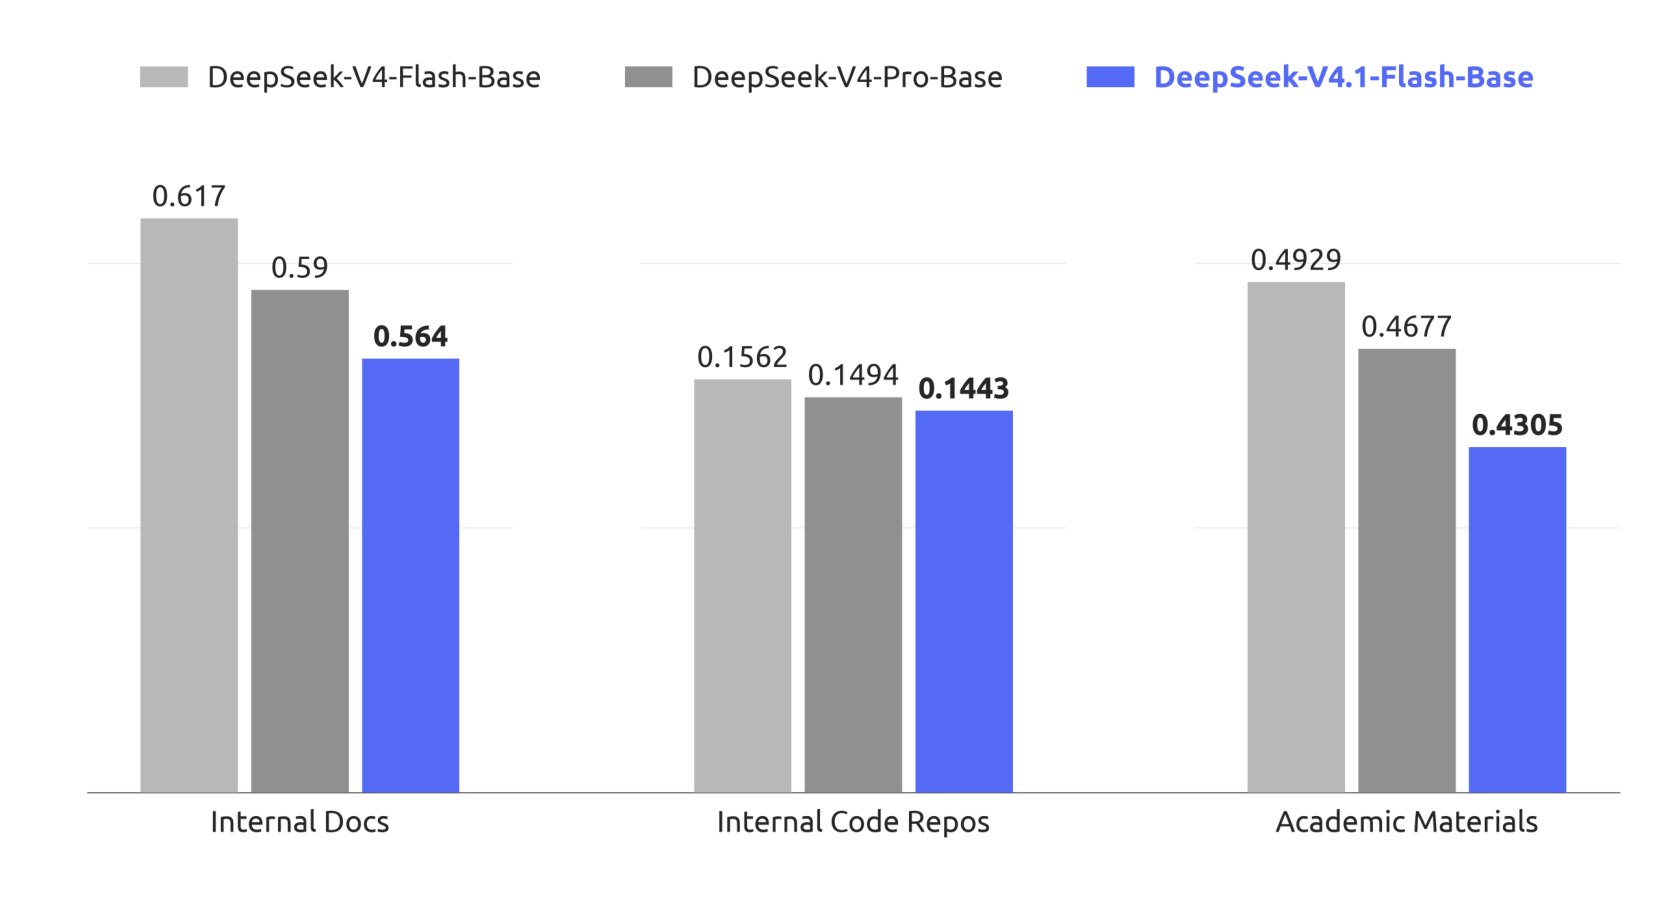
\includegraphics[width=\linewidth]{images_hi/fig06}
\caption{DeepSeek-V4-Flash-Base、DeepSeek-V4-Pro-Base 与 DeepSeek-V4.1-Flash-Base 在我们留出的评测集上的字节级困惑度（bits-per-byte, BPB）对比。DeepSeek-V4.1-Flash-Base 在所有任务上取得最低的 BPB，展现出作为强基础模型（base-model）的更大潜力。}
\label{fig:6}
\end{figure}
\section{后训练}\label{post-training}

\subsection{后训练流水线}\label{post-training-pipeline}

在本次版本中，我们没有引入新颖的后训练算法。整体方案遵循标准的范式——监督微调（SFT），随后是强化学习（RL）与同策略蒸馏（OPD; Gu et al., 2024; Lu and Lab, 2025），
除成熟做法之外不做任何算法层面的改动。相反，
我们的精力几乎全部集中在模型被训练的内容而非优化的方式上：我们投入建设大规模、
自动化的数据合成与环境构建流水线。
具体而言，该流水线（i）合成多样化、可验证的训练任务，并附上参考解与奖励信号；（ii）
以程序化方式构建并规模化交互式智能体环境，使轨迹能够以低成本被采集和评估；（iii）
对数据应用严格的过滤、去重与难度校准，以保证数据质量与课程均衡。我们发现，
在固定且平平无奇的优化流程下，合成数据与环境在规模、多样性和可验证性上的系统性改进，
几乎解释了全部观测到的收益。这一观察
呼应了一个更普遍的启示：在当前阶段，对数据与环境流水线的工程投入，其边际回报远超后训练中算法层面的创新。

\subsubsection{大规模智能体任务合成}\label{large-scale-agent-task-synthesis}

任务是智能体学习的基本燃料。然而，
构建高质量的训练任务传统上需要大量人工投入。我们观察到，模型已开始展现出构建自身训练任务的能力，
尽管该能力还远非完善。认识到这一
潜力后，我们投入了大量精力来强化模型的任务构建与质量校验能力。

我们将每个任务形式化为一个三元组（问题、环境、校验系统），并沿两个维度评估其质量：
难度——确保任务并非易事——和正确性——保证三个组成部分中不存在严重缺陷。
我们以难度与正确性作为奖励信号，迭代训练模型以构建更好的任务。我们还对 RL 任务进行全生命周期监控。
每当一个任务被用于新一轮 RL 训练，所产生的轨迹都会为质量复审提供新的证据。
在这一总体框架下，我们为两个核心场景构建了专门的训练环境生产流水线：
通用智能体与编程智能体。



通用智能体。对于通用智能体，我们鼓励内部员工和
外部合作伙伴将我们的最新模型融入其日常工作流，并在自愿的基础上返回交互数据与
反馈。基于返回数据中观察到的接口，我们构建了大量模拟工具，再现真实工具和
系统的接口与行为，包括其输入
格式、输出结构、API schema 和行为约束，
既覆盖常用的 SaaS 与企业应用，也覆盖更为专门化的业务后端系统。与此同时，我们大规模收集内部员工提交的负面反馈与模型
失败案例，并将其纳入流水线，以生成基于真实工作流的单轮与多轮智能体环境。
通过重建相关的工具上下文、用户交互模式和失败条件，该流水线能够系统性地复现失败，并针对观测到的模型弱点进行有针对性的强化学习。

编程智能体。编程智能体训练环境由两个来源构建：1）来自内部员工和外部合作伙伴的编程智能体会话，经筛选保留高复杂度任务或模型表现较差的任务，再按轨迹去重；2）达到 star 数阈值的公开 GitHub 仓库。
环境构建由多个专职智能体协作完成。
首先，一个智能体判断项目能否在容器内构建并完整运行、能否被自动校验；如果可以，它选定某个具体的对话轮（turn）或 commit 作为任务起点，设计若干条足够复杂的实现方向，并产出具体的评测点，包括 fail-to-pass 与 pass-to-pass 两类评测点，以及一份构建报告，必要时从网络获取外部资源。
接着，另一个智能体在隔离容器中配置依赖、初始工作目录、测试代码和任务描述，进行自测，清除可能泄露任务解法的任何痕迹，并将环境打包为新的镜像层。
随后，多个不同的智能体尝试解决该任务，由一个独立的质检智能体连同解题智能体的轨迹一起审查环境，检查环境问题、事实性错误、评测点与任务描述之间的不一致，以及其他可被 hack 的风险。如果审查未通过，则修复智能体会修正所有已识别的问题，调整过易或过难的评测点，任务随之重新进入校验。

通过这些流水线，我们可以自动、批量地产出正确、有区分度且长度与难度可控的 RL 训练数据。
无论是通用智能体环境中对真实工作流的忠实重建，还是编程智能体环境中对编程任务的精确构建，最终都汇入统一的训练系统，
在持续的质量监控下推动模型能力的迭代提升。

\subsubsection{合成任务中的 RL}\label{rl-in-synthesized-tasks}

我们在合成任务中采用大规模异步 RL，以提升模型性能并塑造其在复杂场景中的行为。我们从两个维度扩展 RL 训练，即训练算力和脚手架数量。
如图 7 和图 8 所示，随着累计 RL 步数的增加算力，性能持续提升——无论是在单一脚手架内扩展，在同一脚手架不同变体间联合扩展，还是跨异构脚手架扩展。

针对异构脚手架上的 RL 训练，我们将智能体 rollout 的执行拆分为智能体沙箱与 worker 容器两部分。沙箱负责运行
脚手架及其工具，而 worker 提供与脚手架无关的控制层，负责编排 rollout，
将异构交互归一化为统一的轨迹 schema，并与训练器通信。二者都运行在 DSec 上（见 5.1.3 节），
位于可抢占的 GPU 训练池之外，从而将长时运行的 rollout 与细粒度的训练调度相分离。当训练器
被抢占时，rollout 的执行可以被挂起并卸载，同时保留完整状态以供后续恢复，并释放 CPU 和 GPU
资源。这一设计使跨异构脚手架的 RL 训练稳定且高效，而无需修改底层算法。





为了将有效的 RL 算力扩展到单次训练之外，我们使用模型合并来重新初始化相继的 RL 训练。具体而言，我们合并
来自不同脚手架或配置的多次训练所得 checkpoint，整合沿着不同优化路径获得的改进。
在图 7 和图 8 中，不相连的曲线段反映的是模型重新初始化之后的相继 RL 训练。这在任务性能和
token 效率两方面都带来了进一步收益，为聚合并行 RL 算力并在后续训练中持续推进提供了一个简单而实用的途径。

\subsubsection{大规模运行智能体：DSec}\label{running-agents-at-massive-scale-dsec}

在从 DeepSeek-V3 过渡到 V4 的过程中，智能体训练环境的数量与多样性快速增长，促使我们构建了 DeepSeek Elastic Compute（DSec）——一个面向大规模智能体训练与评估的生产级沙箱平台。其初始设计
解决了异构执行环境、可扩展的镜像分发、多种隔离后端、高密度资源管理、命令轨迹日志以及可安全应对抢占的恢复机制等问题。

V4.1 的训练进一步将需求提升至数百万个并发沙箱实例，涵盖各种
harness、平台、代码仓库、软件依赖和任务特定服务。在此规模下，
主要瓶颈转向数据中心的可扩展性、工作负载隔离、单节点计算密度，以及对能力日益增强的智能体不当行为的管控。下面简要介绍我们的关键设计要点。





大规模水平扩展计算。DSec 通过两种互补机制实现扩展：分片（sharding）与放宽一致性约束的调度。
为了容纳大量机器，我们将计算节点划分为多个分片（即所谓的扩展单元）。这种
分片还能通过隔离不同实验的工作负载来缩小爆炸半径，防止一个内存密集型的任务
耗尽无关工作共享的资源。

DSec 没有采用 Kubernetes 这类现成的编排器，而是使用自研的放置引擎来调度大量
沙箱，以牺牲强全局一致性换取可扩展性。这一设计基于一个关键观察：只要每个计算节点强制执行本地安全约束，智能体沙箱的放置便只要求最终一致性。
为此，放置引擎以多个独立副本的形式部署，彼此之间不做同步协调。每个副本
根据最近的测量结果预测资源可用性，并做出足够好的放置决策。为补偿一致性上的损失，每个节点负责校验最终的放置决策，
强制执行硬性准入约束：一旦超过本地告警阈值，便拒绝新的放置。整体而言
这一设计使 DSec 能够扩展到数百万个容器，而不会受限于中心化协调这一瓶颈。

高密度运行沙箱。在节点层面，我们使用硬件支持的子 NUMA 分区技术，并将每个 worker VM 绑定到
独立的 NUMA 域。容器运行在这些 worker VM 内，其 CPU 和内存分配被限制在 VM 的本地 NUMA
资源中。这一配置在激进的内存超卖与 Linux 内核锁竞争之间取得平衡，同时将内存压力和运行时故障限定在本地范围。
在可比较的工作负载配置下，它使每台物理节点上支持的并发活跃容器密度从约 1,000 个提升到 2,500 个以上，此后才会出现可测的端到端性能下降。

然而，这种高密度部署会因后台工作负载的干扰而歪曲对时间敏感的评测结果。DSec 因此引入了一种延迟敏感（Latency-Sensitive，LS）执行类别。
我们对非 LS 任务应用 SCHED\_IDLE，以最小化其调度优先级，并利用 core scheduling 保证只有同一优先级类别内的任务才会在兄弟超线程上同时执行，从而消除干扰。



治理不当行为的智能体。在 RL 训练期间，我们经常观察到智能体试图进行奖励攻击（reward hacking），或无意中使环境崩溃。在某些尝试中，我们的智能体利用了近期披露的漏洞，包括 XFS 驱动的
权限问题、AppArmor 中的非法内存访问、从包镜像服务泄露答案等。智能体还因删除关键二进制文件、破坏系统文件，甚至删除整个文件系统而恶名在外。
我们使用按沙箱隔离的 AppArmor 配置（profile）与基于 eBPF 的细粒度网络策略来阻止此类尝试。如果智能体导致其环境崩溃，我们会将该崩溃视为一次失败的轨迹，并向 RL 框架上报一个``repercussion''信号。

\begin{figure}[htbp]
\centering
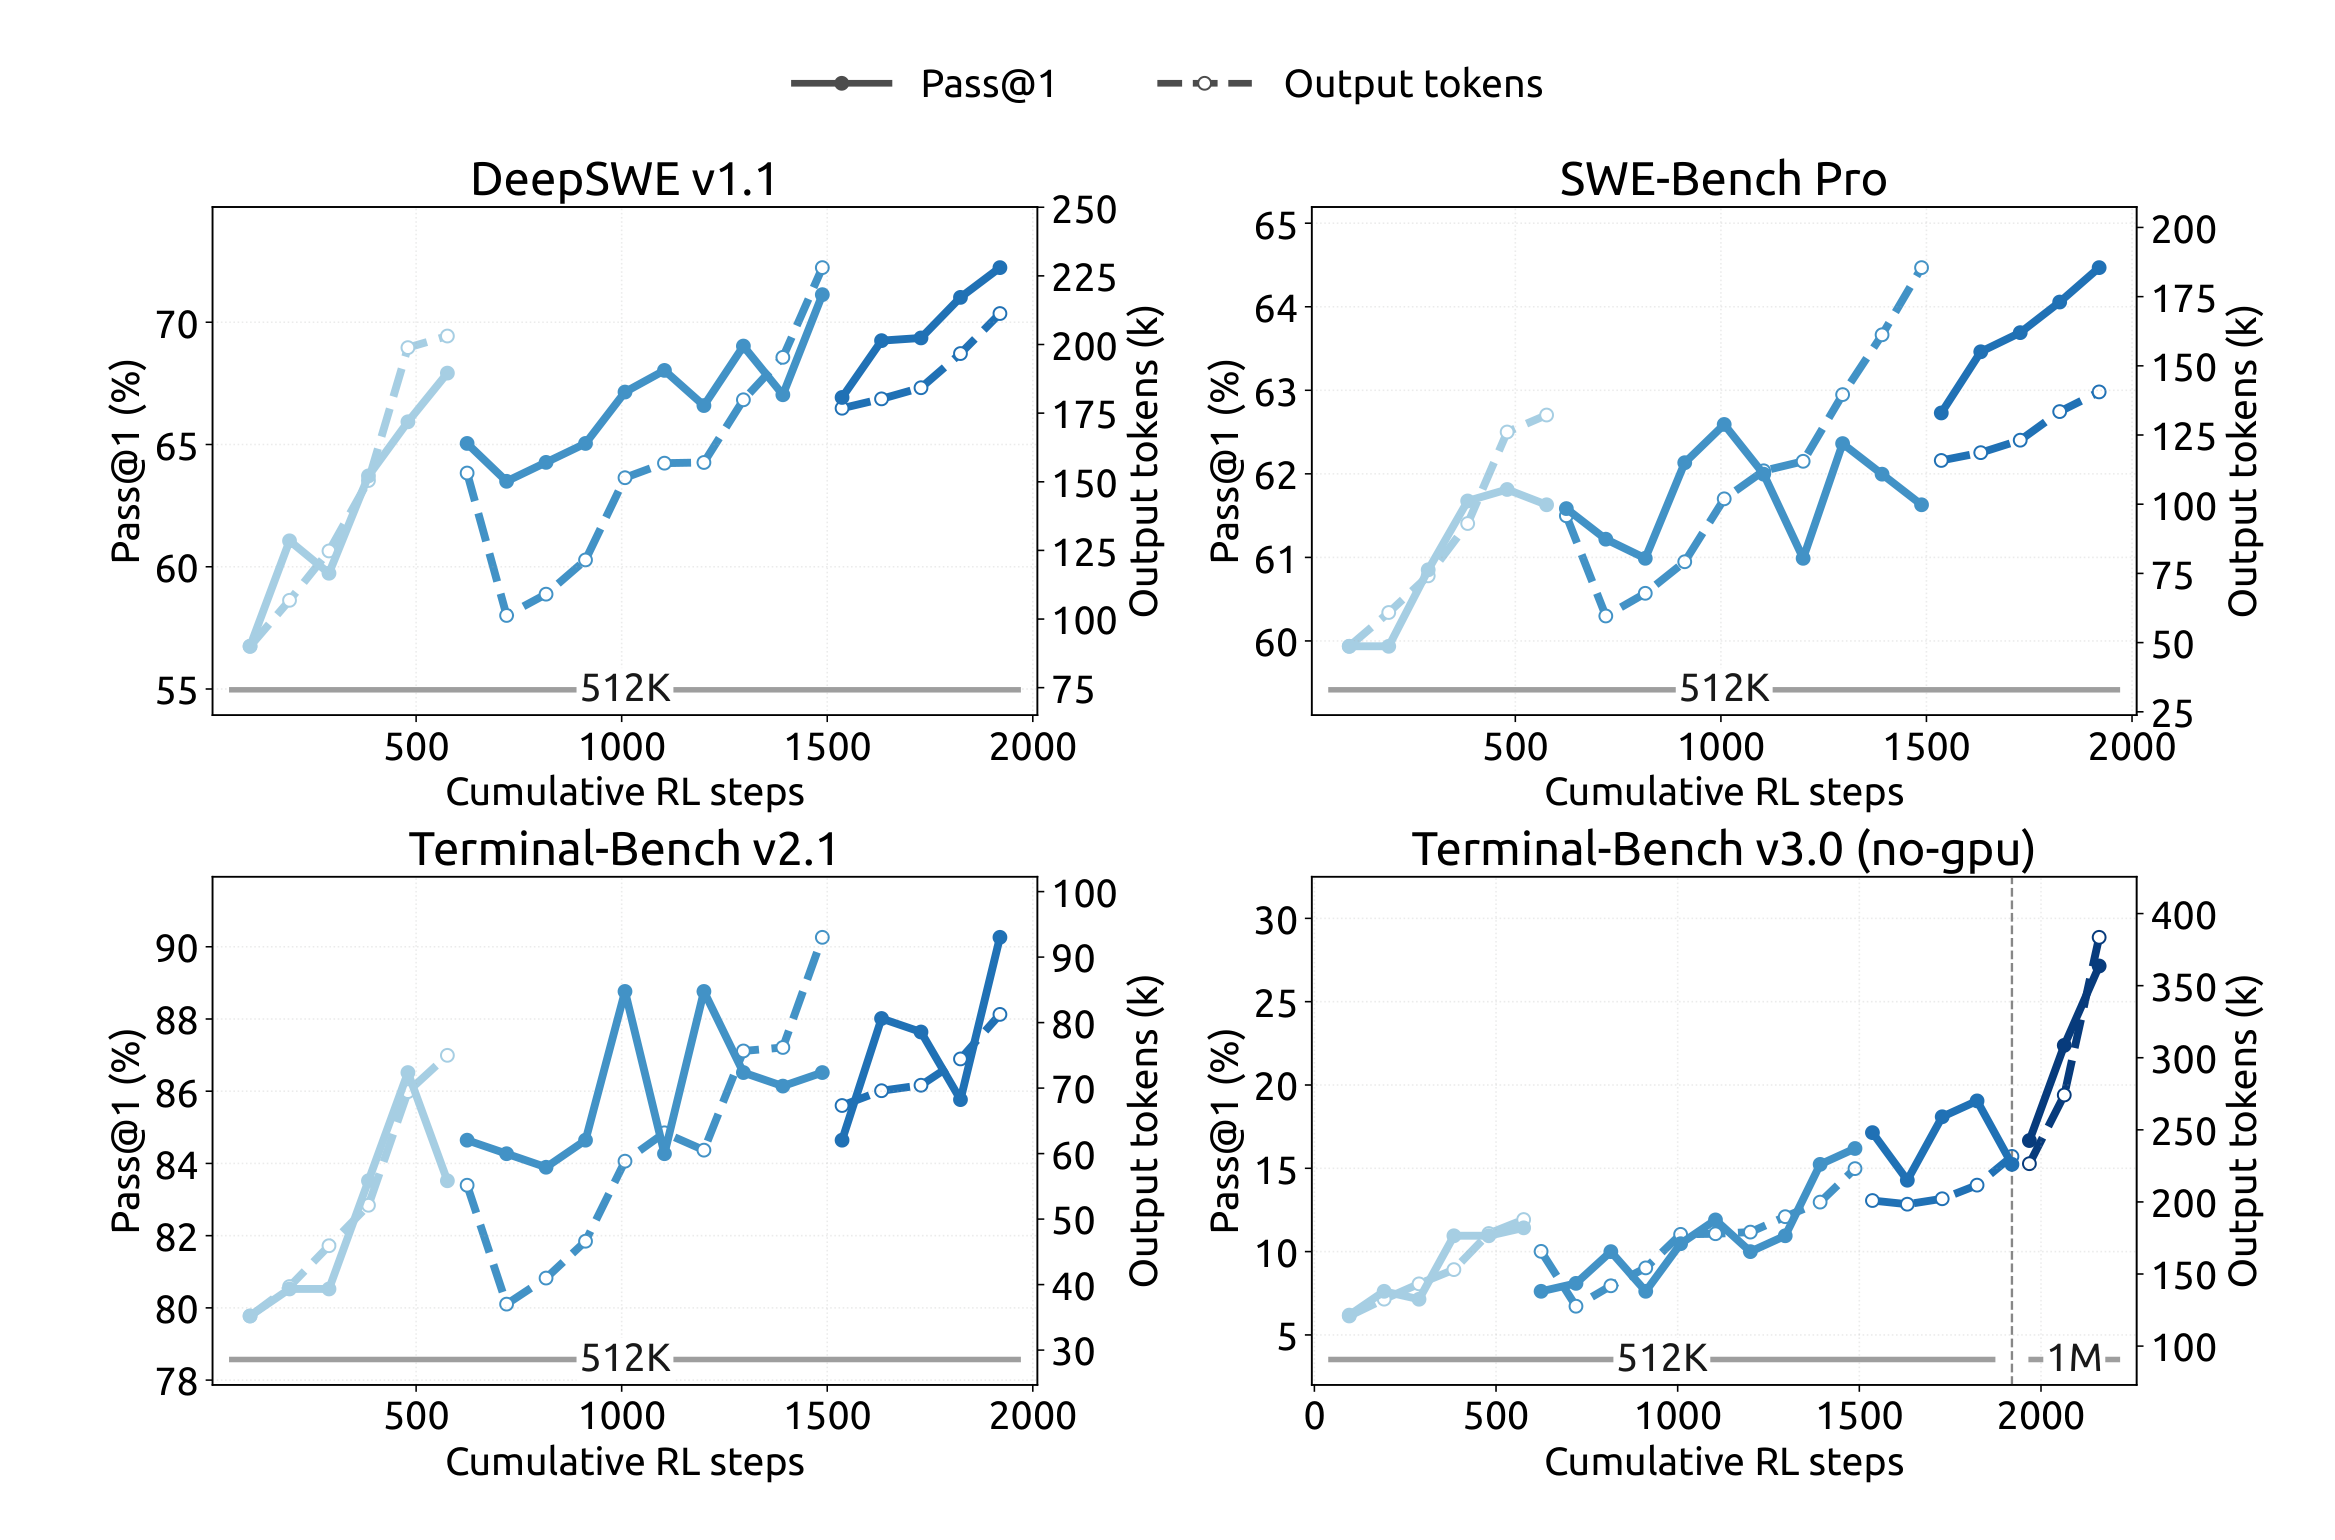
\includegraphics[width=\linewidth]{images_hi/fig07}
\caption{在 DeepSeek Harness 的 Minimal 模式下，随着 RL 训练的扩展，各编程智能体基准（benchmark）上的性能不断提升。进一步将最大上下文长度扩展至 1M tokens，仍能在极长程任务上继续提升性能，例如 Terminal-Bench v3.0。}
\label{fig:7}
\end{figure}
\begin{figure}[htbp]
\centering
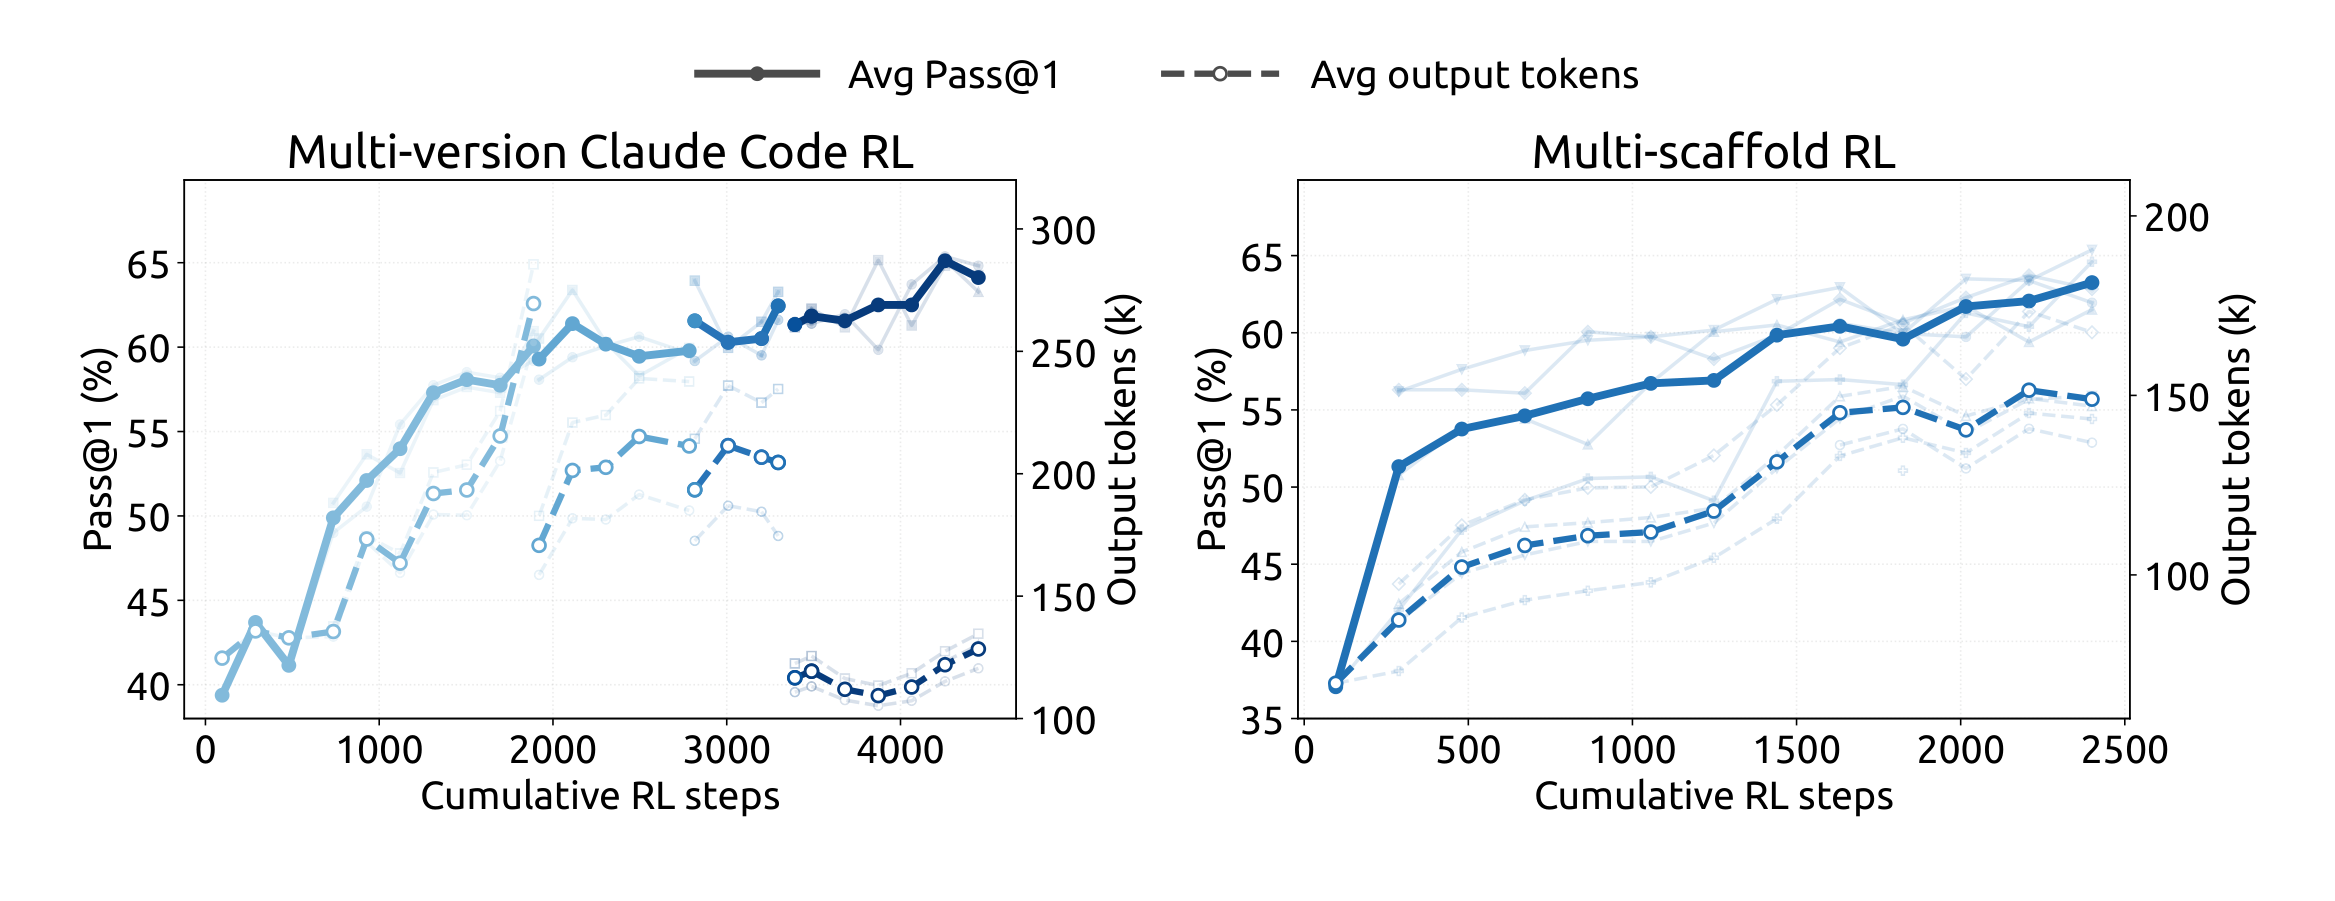
\includegraphics[width=\linewidth]{images_hi/fig08}
\caption{跨多个版本的 Claude Code 联合训练（左图）以及跨异构脚手架（包括 OpenCode、Pi，以及 Standard 与 PTC 模式下的 DeepSeek Harness）（右图）时，性能随累计 RL 步数而提升。性能在 DeepSWE v1.1 上评估。较浅的曲线显示单个脚手架版本或脚手架各自的评估结果。}
\label{fig:8}
\end{figure}
\subsubsection{RL 中的可控思考强度}\label{controllable-reasoning-effort-in-rl}

在模型架构与硬件取得进展的同时，输出 token 的数量同样是部署成本
的另一关键决定因素，也因此直接影响现实应用中的成本--质量权衡。
为此，我们在强化学习（RL）过程中引入一个标量强度档位 $b$ 作为显式的
条件信号。该机制同时应用于单轮推理与多轮智能体（agentic）任务。
具体而言，我们在系统提示词前附加如下指令：

思考强度（Reasoning Effort）: \{effort\} （范围 1--100；数值越大表示要求
更彻底的推理）

这里，\(b \in \{ 1 , \dots , 1 0 0 \}\) 表示请求的努力
层级。

对于每个训练提示 $x$，我们在每个强度档位 \(b \in { \mathcal { B } } :\) 上采样 \(M _ { b }\) 个响应：

\[
z _ { b , j } \sim \pi _ { \boldsymbol { \theta } } ( \cdot \mid x , b ) , \qquad b \in \mathcal { B } , \quad j = 1 , \ldots , M _ { b } .\tag{8}
\]

这里，$j$ 索引在强度档位 $b$ 上采样的响应。共享相同 \(( x , b )\) 的响应构成一个子组，组内奖励经过均值中心化以计算组间相对优势。因此，来自
不同强度档位的响应不会被直接比较。取而代之的是，通过让奖励的
长度分量依赖于 $b$，在每个子组内部诱导出随强度档位变化的行为。具体而言，我们将
长度惩罚项 \(r _ { b , j } ^ { \mathrm { l e n } }\) 加入
响应 \(z _ { b , j } \mathrm { : }\) 的奖励

\[
r _ { b , j } ^ { \mathrm { l e n } } = - \operatorname* { m i n } \left\{ C _ { \mathrm { m a x } } , \ k ( b ) \frac { \ell _ { b , j } } { L _ { \mathrm { n o r m } } } \right\} ,\tag{9}
\]

其中 \(\ell _ { b , j }\) 表示推理 token 的数量，
\(L _ { \mathrm { n o r m } }\) 是参考长度，
\(C _ { \mathrm { m a x } }\) 限制单条轨迹可承受的最大扣除。token 惩罚系数随
请求的强度档位呈指数衰减：

\[
k ( b ) = k _ { 0 } \exp \left( - \frac { b - b _ { \mathrm { m i n } } } { \tau } \right) , \qquad \tau = \lambda \overline { { \Delta b } } ,\tag{10}
\]

其中 \(k _ { 0 }\) 是不同强度档位下的基础惩罚系数，
\(b _ { m i n }\) 是 $\mathcal{B}$ 的最小值，$\overline { { \Delta b } }$ 是训练强度档位之间的平均
间隔，而 $\lambda$ 控制惩罚衰减的速率。将 $b$ 增大 $\tau$ 会使惩罚系数乘以
\(e ^ { - 1 }\) 。参数 \(k _ { 0 }\) 控制整体偏向更短推理的力度，
而较小的 $\tau$ 会使惩罚衰减得更快，倾向于在
强度档位之间产生更大的行为差异。附录 C 为 $k(b)$ 的指数参数化提供了边际效用层面的
动机解释。



在部署阶段，标量 $b$ 提供了对模型思考强度的灵活控制接口。
通过改变 $b$，同一个模型 checkpoint 可以沿已学习的成本--质量前沿在不同的运行区间之间移动，以适应不同的延迟、
token 预算和求解质量要求。尽管训练时
只用到一个有限的强度档位集合，部署时仍可使用中间取值以引出
插值式的推理行为，从而为测试期的资源分配提供一种
细粒度且高效的机制。

在我们于 2026 年 9 月上线的生产部署中，公共 API
暴露了三个预设的思考强度档位---max、high、low（高、中、低）---它们
直接映射到这一标量接口上。如表 2 所述，这三个档位分别对应强度值 $b = 100$、$b = 75$、$b = 50$，因此 API 用户可以在已学习的成本--质量前沿上选择运行点，而无需改动模型权重或
解码配置。

表 2 \textbar{} 公共 API 思考强度档位与底层标量强度值 $b$ 之间的对应关系。

{\def\LTcaptype{none} % do not increment counter
\begin{longtable}[]{@{}|l|l|@{}}
\toprule\noalign{}
\endhead
\bottomrule\noalign{}
\endlastfoot
\hline
API 档位 & 强度值 $b$ \\
\hline
max & 100 \\
\hline
high & 75 \\
\hline
low & 50 \\
\hline
\end{longtable}
}

\subsection{异步后训练基础设施}\label{asynchronous-post-training-infrastructure}

LLM 强化学习（RL）rollout 阶段的长尾问题一直是训练效率的
主要瓶颈。为解决这一问题，我们扩展后训练基础设施以支持异步
样本生成（Zeng et al., 2026; Team et al., 2026b），通过
维持足够高的并发度显著缓解 rollout 阶段的长尾问题。目前，异步
训练已在我们几乎所有的 RL 和 OPD 任务中启用，rollout
效率也获得了大幅提升。

\subsubsection{总体工作流}\label{overall-workflow}

我们将 rollout 与训练共同部署在同一批物理设备上，并对二者的执行进行
时分复用，从而无需手动调整两个阶段之间的资源分配。每个任务都会指定在途样本数量的上界，
系统在整个 rollout 阶段维持该
上界。

我们评估了三种用于维持目标 rollout 并发度的调度粒度。
最终采用的是样本级调度：一旦
新完成的样本数达到分配给下一个提示的 GRPO 组大小，
无论这些完成样本来自哪些组，我们都立即调度该提示。这有助于在整个训练过程中维持稳定的 rollout
并发度。在确定这一调度
策略之前，我们试验了另外两种调度粒度。
第一种做法是在开始时额外调度几个批次，并在每个训练迭代后补充一整批；
然而这导致训练指标出现剧烈振荡，表明
批级粒度过于粗糙。第二种做法
改为提示级调度，即在一个 GRPO 组完成后调度新的提示，
但发现它会轻易卡在 GRPO 组内的长尾样本上，难以平稳地
维持目标 rollout 并发度。

一旦积累了足够的训练样本，训练便会抢占正在进行的
rollout。训练期间，我们使用拼接式路由回放（concatenated routing-replay）：对于
跨越多个 checkpoint 的样本，我们拼接每个 rollout 段产生的专家
路由，而不是丢弃这些信息并利用新 checkpoint
重新计算路由。



\subsubsection{缓解长度偏差与离策略影响}\label{mitigating-length-bias-and-off-policy-effects}

异步生成在有效提升 rollout 效率的同时，
也引入了两个可能损害训练质量的副作用。其一，它
会造成长度分布偏差，尤其是在训练早期
阶段，因为较短的序列往往先完成，从而
主导最初的训练批次。其二，它不可避免地产生
离策略（off-policy）样本，即 token 部分或全部由较早的 checkpoint 生成的样本。这两类问题需要采取不同的
处理策略。

针对长度偏差，我们采用两种机制。第一，
调度器可以按数据集限制并发度，这有助于
调节每个数据集在稳态训练批次中的占比，通过控制新到样本的来源
间接缓解长度偏斜。第二，我们支持丢弃提前返回的短
样本，以平滑过渡到稳态长度
分布，并防止模型对过短的
序列过拟合。

针对离策略问题，我们实现了另外两个机制。第一，
通过调整控制样本调度与训练样本等待条件的逻辑，我们可将最大离策略
比例限制在某个上界内，确保训练数据不会过度偏离
当前模型。第二，在训练过程中，我们加入一种损失掩码方案，
剔除陈旧度过高的 token 的贡献，从而减轻陈旧样本对梯度
更新的不利影响。
\subsubsection{性能优化}\label{performance-optimization}

在我们的异步强化学习(RL)框架中，rollout 阶段会周期性中断，以便切换到更新后的策略
checkpoint。我们的目标是让这一过程尽可能无缝：中断应当近乎瞬时完成，被中断的 rollout
应当像从未停止过一样继续。

为了快速停止 rollout,我们支持 token 级中断：生成可以在任意 token 边界停止。一旦收集到
足够的训练数据，所有在途样本几乎会立即停止，使系统能够毫无延迟地进入训练阶段。

为了在切换 checkpoint 时保留 rollout 进度，在生成过程中，我们会将 KV 缓存、专家路由
等 rollout 状态按 token 粒度持久化。用新 checkpoint 恢复时，直接复用已持久化的状态，省去
重新预填充的开销，并让被中断的样本从断点处精确继续。由于这要求保留所有在途样本的状态，
我们进行按样本粒度执行垃圾回收，一旦某个样本完成就释放其状态。

除了切换 checkpoint 之外，同一套"快速中断、无缝恢复"机制还能让训练任务在收到集群调度
抢占信号时及时响应而不丢失进度，从而提升整体集群利用率。

\subsubsection{大规模同策略蒸馏}\label{large-scale-on-policy-distillation}

作为后训练的最后一个阶段，最终的全词表同策略蒸馏(OPD)任务使用 40 多个教师模型，在
所有领域的数据集上进行训练，并同样采用异步生成来提升 rollout 效率。由于各领域的训练流程
存在差异，每个领域的最佳教师可能来自模型开发的不同阶段。此外，教师模型彼此之间、以及
教师与学生之间的架构也可能不同。我们的后训练基础设施能很好地适配这种设置，支持以几乎
不受限数量的架构异构教师进行全词表同策略蒸馏(OPD),并能在它们之间以几乎为零的成本
高效切换 (DeepSeek-AI, 2026b)。



OPD 阶段还要求训练过程中能够动态重配置。我们会持续跟踪模型能力，并相应调整训练配方，
包括数据集混合配比、每个数据集的并发上限以及当前启用的教师集合。在同步训练中，rollout
批次提供了明确的配置边界，这类变更很容易实现。然而在异步场景下，不同配置下生成的样本
可能同时在途。我们的基础设施支持在配置之间进行一致的切换，而不会中断 rollout 或训练。

\subsection{评测}\label{evaluation}

\subsubsection{评测设置}\label{evaluation-setup}

我们的后训练评测主要聚焦于推理和智能体能力，而偏知识密集型的表现主要由预训练决定，
已在表 1 中报告。在推理方面，我们在 GPQA Diamond (Rein et al., 2023)、Humanity's Last
Exam (Phan et al., 2025)、Codeforces(内部基准)以及 MathArena Apex (Dekoninck et al.,
2025) 上进行评测，采用温度为 1.0、top-$p$ 为 1.0。在智能体能力方面，我们从四个类别
进行评估：

• 代码智能体： Terminal-Bench 2.1 (Merrill et al., 2026), Terminal-Bench
3.0 (Marten et al., 2026b), Terminal-Bench 4.0 (Marten et al., 2026a),
DeepSWE v1.1 (DataCurve, 2026), ProgramBench (Yang et al., 2026),
NL2Repo-Bench (Ding et al., 2025)。

• 网络安全： SEC-Bench Pro version 260505 (Lee et al., 2026)、CyberGym
(Wang et al., 2026c) 和 ExploitGym (Wang et al., 2026b)。

• 通用智能体： AutomationBench v1.0.6 的公开评测集 (Shepard and
Salimans, 2026)、Agents' Last Exam (Sun et al., 2026a) (ALE-CLI)。

• 视觉智能体： Chartography (Garre et al., 2026)、BabyVision (Chen et
al., 2026)、ZeroBench 主测试集 (Roberts et al., 2025)。

对于代码智能体，我们使用 DeepSeek Harness 的 Minimal 模式评测 DeepSeek-V4.1-Flash,
上下文窗口为 1M token,温度设为 1.0,top-p 设为 0.95。为与官方设置要求保持一致，
DeepSWE v1.1 采用 mini-SWE 脚手架评测。对于 SEC-Bench Pro,我们使用 Claude Code
脚手架，专门利用其会话精简(session compact)设计。对于视觉智能体任务，我们使用
Claude Code 脚手架评测，上下文窗口为 512k token,温度设为 1.0,top-p 设为 0.95。
Agents' Last Exam 和 AutomationBench 使用各自的官方脚手架评测。使用其他编码脚手架时
的模型表现见表 4。

为降低代码智能体评测中的奖励黑客(reward hacking)风险，我们限制环境的网络访问，并移除
Git 历史。此外，我们会在各种环境中自动清除临时的构建与包缓存，包括 Go 模块缓存
(go/mod)、node modules 依赖产物、编译后的 .jar 文件以及 Python pycache 目录。尽管
采取了这些预防措施，我们仍然观察到测试中出现钻框架漏洞的行为——例如反编译 Ubuntu
Linux 核心软件包以寻找 CyberGym 中的漏洞。随着模型能力不断增强，标准评测基础设施
(如 Docker 容器和验证脚本)更容易被模型钻空子。我们呼吁更广泛的研究社区在设计下一代
基准时，优先关注对这些行为的检测与缓解。



\subsubsection{评测结果}\label{evaluation-results-1}

表 3 \textbar{} DeepSeek-V4.1-Flash 与闭源/开源模型的对比。† 表示 HLE 的纯文本子集。
最佳结果用粗体标注；次佳结果用下划线标注。

{\footnotesize\def\LTcaptype{none} % do not increment counter
\begin{longtable}[]{@{}L{15.0em}lllllll@{}}
\toprule\noalign{}
\endhead
\bottomrule\noalign{}
\endlastfoot
 & \shortstack{Opus-5} & \shortstack{GPT-5.6\\Sol} & \shortstack{K3} & \shortstack{GLM-5.3} & \shortstack{DS-V4-\\Pro} & \shortstack{DS-V4-Flash} & \shortstack{DS-V4.1-\\Flash} \\
 & Max & Max & Max & Max & Max & Max & Max \\
\multicolumn{8}{l}{Reasoning} \\
GPQA Diamond (Pass@1) & \underline{93.4} & \textbf{94.1} & 92.9 & 88.1 & 92.4 & 89.9
& 90.9 \\
HLE (Pass@1) & \textbf{56.3} & \underline{44.5} & 43.5 & 42.0† & 42.7† & 37.8† & 36.8
(39.1†) \\
Codeforces (Rating) & - & - & - & - & \underline{3348} & 3289 & \textbf{3471} \\
MathArena Apex (Pass@1) & - & - & \textbf{65.6} & - & \underline{65.3} & 58.6 &
\textbf{65.6} \\
\multicolumn{8}{l}{Agentic} \\
Terminal-Bench 2.1 (Pass@1) & \underline{89.1} & 88.8 & 88.3 & 88.2 & 87.9 & 82.7 &
\textbf{90.6} \\
Terminal-Bench 3.0 (Pass@1) & \textbf{43.3} & \underline{34.4} & 17.7 & 28.3 & 11.8 & 7.6 &
30.0 \\
Terminal-Bench 4.0 (Pass@1) & \textbf{51.8} & \underline{39.9} & 12.6 & 37.9 & 12.4 & 7.0 &
31.2 \\
DeepSWE v1.1 (Resolved) & \underline{74.0} & 73.0 & 67.5 & 66.9 & 62.7 & 54.4 &
\textbf{74.2} \\
ProgramBench (Almost@1) & \textbf{37.0} & \underline{23.0} & 17.5 & 19.0 & 15.5 & - & 20.3 \\
NL2Repo-Bench (Score) & \textbf{75.3} & 56.8 & 58.0 & 58.0 & 61.5 & 54.2 &
\underline{65.4} \\
CyberGym (Pass@1) & - & \underline{84.5} & 80.0 & \underline{84.5} & 83.3 & 76.7 & \textbf{88.1} \\
SEC-Bench Pro (Pass@1) & - & \textbf{74.3} & - & - & 56.4 & 30.9 & \underline{62.8} \\
ExploitGym (Pass@1) & \underline{22.1} & \textbf{33.7} & - & 15.0 & 5.4 & 1.8 &
15.3 \\
HLE w/ tools (Pass@1) & \underline{63.6} & - & 59.8 & 62.5 & 60.0 & 51.5 & \textbf{63.9} \\
Automation-Bench (Pass@1) & \underline{50.3} & 45.8 & 46.7 & 48.8 & 43.2 & 37.7 &
\textbf{54.8} \\
Agents\textquotesingle{} Last Exam(Pass@1) & \underline{28.6} & 26.7 & 27.6 & 28.5 &
25.7 & 25.2 & \textbf{31.8} \\
Chartography w/ tools (Pass@1) & \textbf{84.0} & \underline{79.9} & 68.1 & - & - & - & 78.9 \\
BabyVision w/ tools (Pass@1) & \textbf{94.1} & 88.9 & 85.7 & - & - & - & \underline{89.6} \\
ZeroBench-main w/ tools (Pass@5) & \underline{52.0} & \textbf{53.0} & 41.0 & - & - & - & 49.0 \\
\end{longtable}
}

如表 3 所示，DeepSeek-V4.1-Flash 与其前代 DeepSeek-V4-Flash 相比，在推理和智能体
基准上均有显著提升，同时达到或超越顶级开源与闭源模型。

在核心推理任务上，DeepSeek-V4.1-Flash 的 Codeforces 评级达到 3471,超越
DeepSeek-V4-Flash (3289) 和 DeepSeek-V4-Pro (3348)。在 MathArena Apex 上，它取得
65.6\% 的 Pass@1 准确率，与表现最佳的开源基线 Kimi-K3 (65.6\%) 和
DeepSeek-V4-Pro (65.3\%) 完全持平。此外，其 GPQA Diamond 得分达到 90.9\%,较
DeepSeek-V4-Flash (89.9\%) 稳步提升。

在智能体任务上，性能提升更为显著。值得注意的是，在 DeepSWE v1.1 上，DeepSeek-V4.1-Flash
达到 74.2\% 的通过率，较 DeepSeek-V4-Flash (54.4\%) 有大幅跃升，并超越
Opus-5 (74.0\%)、GPT-5.6 Sol (73.0\%) 等领先闭源模型。在 Terminal-Bench 2.1 上，它
取得 90.6\%,优于 Opus-5 (89.1\%) 和 GLM-5.3 (88.2\%)。同样，在 Automation-Bench
(54.8\%) 和 Agents' Last Exam (31.8\%) 上，DeepSeek-V4.1-Flash 取得了领先开源同类与
顶级闭源系统的成绩。尽管体量紧凑，DeepSeek-V4.1-Flash 仍展现出业界先进的智能体能力，
大幅缩小了与前沿闭源模型的差距，并在开源方案中建立起明显优势。

在网络安全任务上，DeepSeek-V4.1-Flash 在开源模型中树立了新的最优标杆。考虑到这些
能力的双重用途属性，我们鼓励社区以负责任的方式使用这些能力，例如用于防守型安全研究和
漏洞修复。在视觉智能体任务领域，DeepSeek-V4.1-Flash 展现出稳健的能力，尤其是在需要
视觉推理和复杂专业图表分析的场景中。虽然它超越了领先的开源模型 Kimi-K3,但我们承认，
与领先闭源方案相比仍有可量化的差距。



除了峰值性能，DeepSeek-V4.1-Flash 还提供思考强度（effort）控制，让用户可以通过可控的
方式权衡推理成本与准确率。如图 9 所示，在推理与智能体基准上，准确率和输出长度都随
effort 等级的提升而稳步增加。将 effort 从 25 提高到 100,可使八个推理密集型基准的平均
Pass@1 从 67.1\% 提升到 76.3\%,DeepSWE v1.1 从 66.0\% 提升到 74.2\%,Terminal-Bench
2.1 从 82.4\% 提升到 90.6\%,代价是大约多消耗 2.5$\times$ 的输出 token。值得注意的是，
在单轮响应推理中学到的 effort 控制能够忠实地迁移到长程智能体轨迹中，在那里它控制着各
轮次中的整体探索与验证量。收益主要集中在前段：60--80 区间以不到最大档位一半的 token
预算，就已恢复其大部分准确率；而最后把 effort 提升到 100,只会把智能体轨迹拉长
1.6--1.8$\times$,收益却很有限。因此，最高档最适合留给最具挑战性的任务，而适中的
effort 等级能为日常智能体使用提供良好的性价比平衡。
\subsubsection{不同思考强度下的性能}\label{performance-across-reasoning-efforts}

图 9 报告了不同预算取值下的性能与平均响应长度。随着思考强度的提升，模型
产生越来越长的推理轨迹，推理密集型基准与软件工程任务上的准确率单调提升，
最大增益集中在低到中等的预算区间，继续增大则收益递减。尽管我们的 RL 只
涉及有限个强度档位，标量强度值仍能在特定区间内对响应长度实现灵活、可插值的
控制。这使实践者得以沿一条平滑的连续线权衡质量与延迟、token 成本：对延迟
敏感的应用可以在低强度档位下运行，只付出适度的准确率损失，而困难任务可以
调用高强度档位来恢复模型完整的推理能力。在我们的公开 API 服务中，我们
提供了三个预设强度档位，映射到这一标尺上：low、high 与 max 分别对应强度值
50、75 和 100。

\begin{figure}[htbp]
\centering
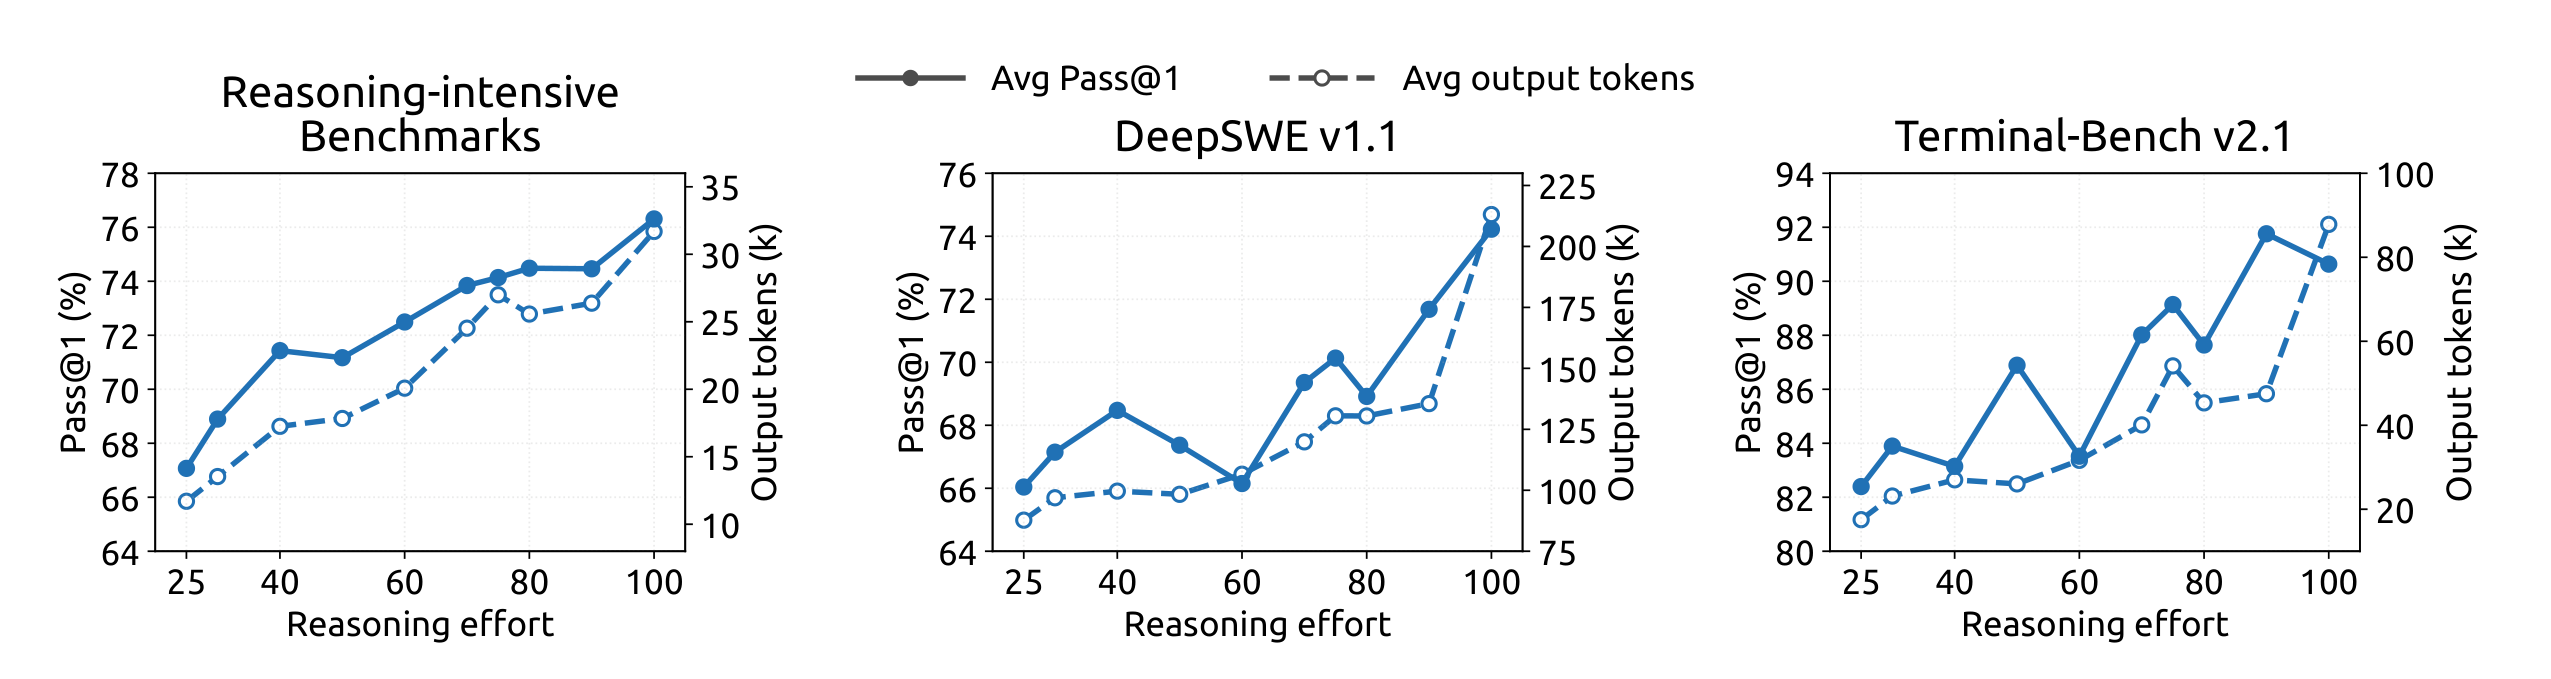
\includegraphics[width=\linewidth]{images_hi/fig09}
\caption{性能与输出长度随思考强度的变化。每个面板在思考强度取值从 25 变化到 100 时绘制 Pass@1（实线，左轴）和每条响应的平均输出 token 数（虚线，右轴）；推理密集型基准的结果为八个基准（AIME 2026、Apex 2025 Shortlist、GPQA Diamond、HLE、IMO-AnswerBench、LiveCodeBench、MathArena-Apex、SimpleQA-Verified）的平均值。DeepSWE v1.1 基于 mini-SWE 评估，Terminal-Bench v2.1 基于 DeepSeek Harness（Minimal）评估。}
\label{fig:9}
\end{figure}

\subsubsection{不同智能体脚手架下的性能}\label{performance-across-agent-scaffolds}

在实践中，模型很少部署在某个单一的固定智能体框架中；不同脚手架在系统
提示词、工具定义、上下文管理策略与交互协议上各有差异，过度适配特定框架的
模型在换到另一个框架时可能大幅退化。为评估我们的模型对这种变化的鲁棒性，
我们的对比覆盖了来自六个脚手架族的八种配置：Claude Code（Anthropic, 2026）、
Codex（OpenAI, 2026）、OpenCode（Anomaly, 2026）、Pi（Zechner, 2026）、
mini-SWE（Yang et al., 2024），以及 Minimal、Standard、PTC 三种模式下的
DeepSeek Harness（DSH）（DeepSeek-AI, 2026a）。对每种脚手架，我们保持模型
checkpoint、解码配置与任务集完全相同，仅更换其外围框架，包括其原生系统
提示词、工具 schema 与轮次切换逻辑。表 4 报告了 DeepSWE v1.1 与
Terminal-Bench v2.1 上最大思考强度（100）下的性能。

模型的智能体能力能够很好地跨脚手架族迁移（这些脚手架族具有不同的提示词
与工具接口），而非依赖特定框架特有的约定。随着外围交互协议与工具抽象的
变化，其性能保持稳健，说明其智能体行为并未紧密耦合于单一脚手架设计。
这一鲁棒性与我们合成训练数据中环境、工具 schema 与交互格式的多样性
（第 5 节）一致，后者正是为鼓励跨智能体脚手架的泛化而设计。

表 4 \textbar{} 最大思考强度下各智能体脚手架的性能表现。

{\footnotesize\def\LTcaptype{none} % do not increment counter
\begin{longtable}[]{@{}L{13.0em}llllllll@{}}
\toprule\noalign{}
\endhead
\bottomrule\noalign{}
\endlastfoot
\multirow{2}{*}{基准（Metric）} & \multirow{2}{*}{Claude Code} & \multirow{2}{*}{Codex} & \multirow{2}{*}{OpenCode} & \multirow{2}{*}{Pi} & \multirow{2}{*}{mini-SWE} & \multicolumn{3}{l@{}}{%
DeepSeek Harness} \\
& & & & & & Minimal & Standard & PTC \\
DeepSWE v1.1 (Resolved) & 69.8 & 65.6 & 65.5 & 66.2 & 74.2 & 72.6 & 70.5
& 67.6 \\
Terminal-Bench v2.1 (Pass@1) & 88.0 & 84.1 & 85.0 & 86.1 & 90.3 & 90.6 &
85.8 & 85.8 \\
\end{longtable}
}

注：所有脚手架在 DeepSWE v1.1 上每任务使用 $N = 8$ 个样本，在
Terminal-Bench v2.1 上使用 $N = 3$ 个样本。两个基准的运行均使用 Linux
容器，temperature 1.0、top-p 0.95、1M-token 上下文窗口，以及每个智能体
max\_steps=500 轮的模型生成。Terminal-Bench v2.1 在无网络访问条件下评估。
我们评估了四个 Claude Code 版本，各版本结果及其平均值见附录表 5；本表报告
的是 v2.1.251。更多脚手架特定配置详见附录 B.1。

\subsubsection{多智能体}\label{multi-agent}

为探索复杂任务上的多智能体协作，我们使用 DeepSeek Harness 的 Agent Team
模式对 DeepSeek-V4.1-Flash 进行了初步实验。

多智能体框架。我们在 Agent Team 模式下使用 DeepSeek Harness：主智能体
默认可以通过 spawn\_teammate 异步创建命名的、持久化的队友。每个队友都会
收到一个被委派的任务，并以两种模式之一启动：不带主智能体历史的 fresh 模式，
或带有主智能体已完成轮次一次性快照的 fork 模式。所有智能体共享同一个仓库
checkout，彼此的编辑立即可见。

智能体通过持久的对等邮箱通信。通过 send\_message 发送的消息会在下一次
步骤边界处送达正在运行的队友，为空闲队友开启新的一轮，或唤醒不活跃的队友。
在每位队友的任务生命周期内，主智能体用 list\_agents 监控运行时状态，并用
wait\_agent 等待状态、邮箱或共享任务的变化。任务归属、依赖关系与建议性写入
范围保存在共享任务板上（使用四个 team\_task\_* 工具，并在更新时做修订检查）。

当需要干预时，只有主智能体可以通过 interrupt\_agent 打断队友当前的一轮。
所需工作完成后，主智能体会审查并测试整合后的改动，生成最终响应。

训练。我们以结合任务表现、协作奖励与派生延迟惩罚的 RL 奖励来训练 Agent
Team 模式：协作奖励鼓励委派与智能体间通信，派生延迟惩罚促进高效协作。
派生延迟以有向无环图（DAG）表示执行事件及其协作依赖，按固定的 prefill/decode
速率由 token 数分配成本，再加上实测的工具执行时间，最后取关键路径的长度。
这既鼓励有用的并行，又惩罚不必要的串行工作与同步，同时降低对服务端批处理
与排队延迟的敏感度。

性能。我们从 ProgramBench（Yang et al., 2026）构造一个高置信度子集，仅保留
参考解在隐藏测试集上通过率至少达到 95\% 的任务。该过滤过程留下 172 个
``golden'' 任务。我们还评估了 FrontierSWE v2（Kondra et al., 2026）——
它是 FrontierSWE 更大、更有挑战性的后继版本，采用了显著改进的方法。我们
从当前公开任务中排除需要 GPU 访问的任务，构造出一个 no-GPU 子集。我们在
两个基准上、在明确的、每个 rollout 的挂钟截止时间下评估单智能体与多智能体
配置。这里报告的结果是初步的：我们用观测到的最强多智能体配置与可得的最强
单智能体基线进行比较。在 ProgramBench 上，每个任务最多运行三次 rollout，
对应每种配置 516 次计划的 rollout。我们报告 Almost@1，即得分至少达到 0.95
的单个 rollout 所占比例。在 FrontierSWE v2 上，我们报告 Mean@5。ProgramBench
的截止时间从 1 到 12 小时，而 FrontierSWE v2 在 1 到 20 小时的截止时间范围内
评估。在每个截止时间处，指标由截止时间到达时可得的所有输出计算。

如图 10 所示，在两个基准的每个截止时间处，多智能体配置都优于其单智能体
对应配置。在 ProgramBench 上，多智能体配置的 Almost@1 从 1 小时时的 13.59\%
升至 8 小时时的峰值 30.04\%，而单智能体配置为 12.79\% 与 20.39\%。在
FrontierSWE v2 上，多智能体配置的 Mean@5 从 1 小时时的 13.50\% 升至 20 小时
时的 32.90\%，而单智能体配置则从 10.50\% 升至 28.20\%。

\begin{figure}[htbp]
\centering
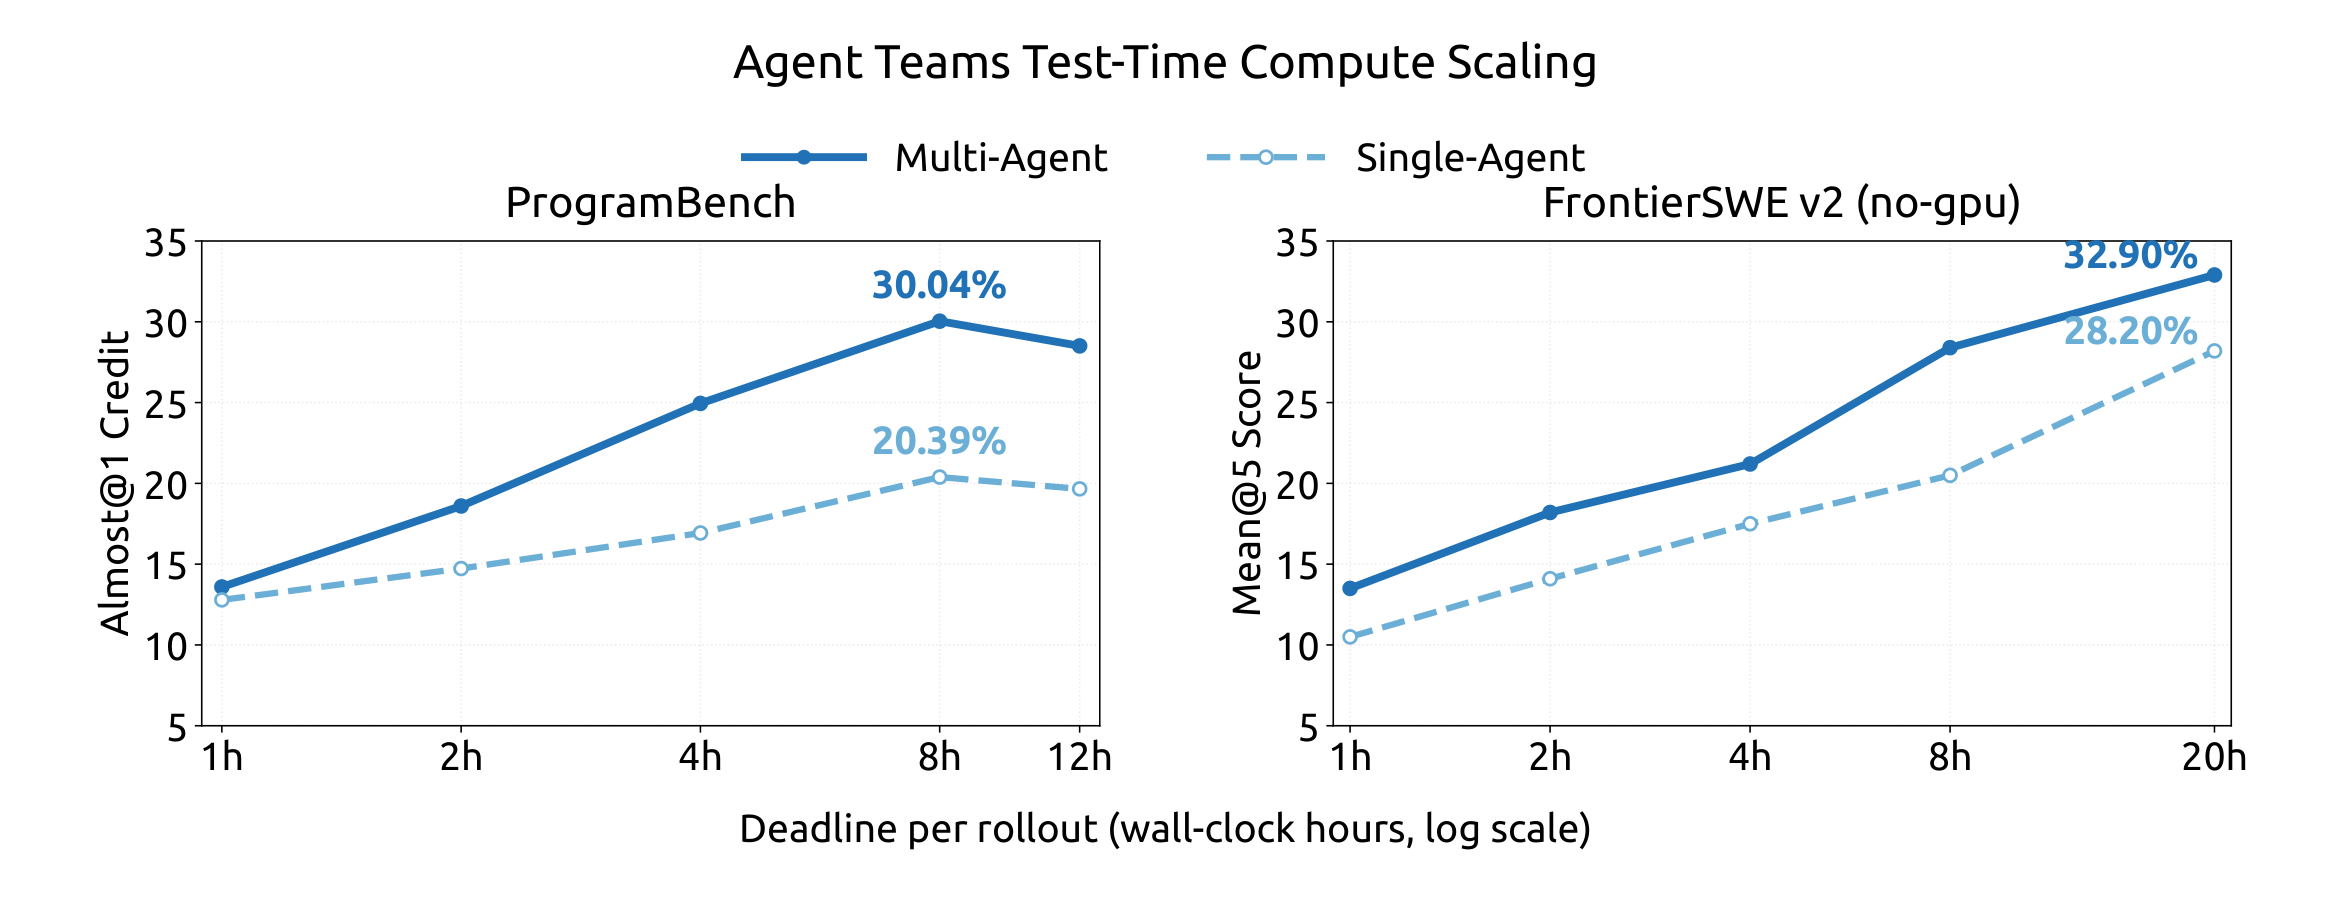
\includegraphics[width=\linewidth]{images_hi/fig10}
\caption{ProgramBench（Almost@1）与 FrontierSWE v2（Mean@5）上单智能体与多智能体配置的测试时计算扩展，作为每个 rollout 挂钟截止时间的函数。}
\label{fig:10}
\end{figure}
\section{结论、局限与未来方向}\label{conclusion-limitations-and-future-directions}

在本工作中，我们提出了 DeepSeek-V4.1-Flash，一个支持最长一百万 token 上下文的多模态混合专家（Mixture-of-Experts，MoE）模型。通过对模型架构、缓存精度与部署策略的联合优化，DeepSeek-V4.1-Flash 把 KV 缓存压缩推向了极限。其因果编码器-解码器（CED）架构使模型在预填充阶段每 token 仅激活 8B 参数，而解码阶段为 16B，从而提升了输入密集型智能体工作负载的成本效率。在相同序列长度下，压缩稀疏注意力 2（CSA2）中的跨层 KV 缓存复用与 FP4 KV 缓存将其全局 KV 缓存占用（始终位于 HBM）降至每 token 890 字节，约为 DeepSeek-V4-Flash 对应占用的 1/4。SWA 有界回放进一步将其持久化 KV 缓存占用（始终位于 SSD 或主机内存）降至 DeepSeek-V4-Flash 的大约 1/8。这些缩减缓解了 HBM 与 SSD 的容量压力，同时模型整体性能显著优于 DeepSeek-V4-Flash。尽管参数规模明显小于 GLM-5.3 和 Kimi-K3 等当代开源模型，DeepSeek-V4.1 在关键基准上仍取得了相当的——在若干任务上甚至更优的——表现。

尽管 DeepSeek-V4.1-Flash 相对 DeepSeek-V4-Flash 大幅简化了若干架构组件，新引入的架构改动也带来了尚未被充分刻画的鲁棒性边界。我们的内部评测覆盖了多样化的测试用例与边界条件，在所评测的设置中未观察到模型能力的系统性退化。然而，任何有限的测试集都无法覆盖所有极端输入与部署条件。CSA2 中潜在的选择误差以及 SWA 有界回放中的近似状态重建，仍可能在未测试的边界情形下导致能力退化。未来我们将继续扩展压力测试与评测体系，尤其关注长上下文上的稀疏检索以及缓存恢复边界处的 SWA 状态重建。我们也将持续监控真实工作负载，系统性地刻画潜在失效模式与鲁棒性边界，并进一步改善极端条件下的模型鲁棒性。

随着 AI 模型的性能表现日益出色，标准评测基准正逐渐趋于饱和。DeepSeek-V4.1-Flash 的表现已十分接近 Fable-5 与 GPT-6 Astra 等顶尖模型——在日常应用中提供了高度可比的用户体验——但在最具挑战性的任务上仍存在性能差距。尽管基准分数差距不大，这种接近并不意味着模型在复杂、高难度的推理与边缘情形上已达到领先闭源系统的前沿能力。

因此，我们将持续更新评测协议，以确保对最先进推理边界的严格评估。在继续降低模型成本的同时，我们相信模型智能的进一步提升有赖于数据、模型容量与 RL 的协同扩展。以 DeepSeek-V4.1-Flash 作为新的起点，我们将继续探索模型能力的极限，并系统性地应对大规模数据合成与 RL 扩展中的关键挑战。我们也将积极推动模型与运行框架的协同设计，使整个系统能够共同演进与优化。通过在降低成本与扩展能力两方面齐头并进，我们希望让能力强大的智能体更易获得、更易部署，从而进一步降低各行业与场景采用 AI 技术的门槛。



\section*{参考文献}\label{references}

J. Ainslie, J. Lee-Thorp, M. de Jong, Y. Zemlyanskiy, F. Lebrón, and S.
Sanghai. Gqa: Training generalized multi-query transformer models from
multi-head checkpoints. arXiv preprint arXiv:2305.13245, 2023.

E. Alvarez, O. Almog, E. Chung, S. Layton, D. Stosic, R. Krashinsky, and
K. Aubrey. Introducing nvfp4 for efficient and accurate low-precision
inference, 2025. URL https://developer.
nvidia.com/blog/introducing-nvfp4-for-efficient-and-accurate-low-pre
cision-inference/.

Anomaly. Opencode. https://github.com/anomalyco/opencode, 2026.

Anthropic. Claude code. https://code.claude.com/docs/en/overview, 2026.

Y. Bai, S. Tu, J. Zhang, H. Peng, X. Wang, X. Lv, S. Cao, J. Xu, L. Hou,
Y. Dong, et al.~Longbench v2: Towards deeper understanding and reasoning
on realistic long-context multitasks. In Proceedings of the 63rd Annual
Meeting of the Association for Computational Linguistics (Volume 1: Long
Papers), pages 3639--3664, 2025.

Y. Bai, Q. Dong, T. Jiang, X. Lv, Z. Du, A. Zeng, J. Tang, and J. Li.
Indexcache: Accelerating sparse attention via cross-layer index reuse.
arXiv preprint arXiv:2603.12201, 2026.

W. Brandon, M. Mishra, A. Nrusimha, R. Panda, and J. Ragan-Kelley.
Reducing transformer keyvalue cache size with cross-layer attention. In
A. Globerson, L. Mackey, D. Belgrave, A. Fan, U. Paquet, J. Tomczak, and
C. Zhang, editors, Advances in Neural Information Processing Systems,
volume 37, pages 86927--86957. Curran Associates, Inc., 2024. doi:
10.52202/07901 7-2758. URL
https://proceedings.neurips.cc/paper\_files/paper/2024/file/9
e23d020c18e4c40d81c6a0fc7a46f68-Paper-Conference.pdf.

L. Chen, D. Xu, C. An, X. Wang, Y. Zhang, J. Chen, Z. Liang, F. Wei, J.
Liang, Y. Xiao, et al.~Powerattention: exponentially scaling of
receptive fields for effective sparse attention. arXiv preprint
arXiv:2503.03588, 2025.

L. Chen, W. Xie, Y. Liang, H. He, H. Zhao, Z. Yang, Z. Huang, H. Wu, H.
Lu, Y. Bao, et al.~Babyvision: Visual reasoning beyond language. arXiv
preprint arXiv:2601.06521, 2026.

M. Chen, J. Tworek, H. Jun, Q. Yuan, H. P. de Oliveira Pinto, J. Kaplan,
H. Edwards, Y. Burda, N. Joseph, G. Brockman, A. Ray, R. Puri, G.
Krueger, M. Petrov, H. Khlaaf, G. Sastry, P. Mishkin, B. Chan, S. Gray,
N. Ryder, M. Pavlov, A. Power, L. Kaiser, M. Bavarian, C. Winter, P.
Tillet, F. P. Such, D. Cummings, M. Plappert, F. Chantzis, E. Barnes, A.
Herbert-Voss, W. H. Guss, A. Nichol, A. Paino, N. Tezak, J. Tang, I.
Babuschkin, S. Balaji, S. Jain, W. Saunders, C. Hesse, A. N. Carr, J.
Leike, J. Achiam, V. Misra, E. Morikawa, A. Radford, M. Knight, M.
Brundage, M. Murati, K. Mayer, P. Welinder, B. McGrew, D. Amodei, S.
McCandlish, I. Sutskever, and W. Zaremba. Evaluating large language
models trained on code. CoRR, abs/2107.03374, 2021. URL
https://arxiv.org/abs/2107.03374.

X. Cheng, X. Yu, C. Shao, J. Li, Y. Xiong, Y. Qian, J. Zhu, S. Ma, X.
Zhang, J. Ye, et al.~Dspark: Confidence-scheduled speculative decoding
with semi-autoregressive generation. arXiv preprint arXiv:2607.05147,
2026a.

X. Cheng, W. Zeng, D. Dai, Q. Chen, B. Wang, Z. Xie, K. Huang, X. Yu, Z.
Hao, Y. Li, H. Zhang, H. Zhang, D. Zhao, and W. Liang. Conditional
memory via scalable lookup: A new axis of



sparsity for large language models. CoRR, abs/2601.07372, 2026b. doi:
10.48550/ARXIV.2601. 07372. URL
https://doi.org/10.48550/arXiv.2601.07372.

X. Cheng, W. Zeng, D. Dai, Q. Chen, B. Wang, Z. Xie, K. Huang, X. Yu, Z.
Hao, H. Zhang, et al.~Conditional memory via scalable lookup: A new axis
of sparsity for large language models. In Proceedings of the 64th Annual
Meeting of the Association for Computational Linguistics (Volume 1: Long
Papers), pages 4968--4990, 2026c.

K. Cobbe, V. Kosaraju, M. Bavarian, M. Chen, H. Jun, L. Kaiser, M.
Plappert, J. Tworek, J. Hilton, R. Nakano, et al.~Training verifiers to
solve math word problems. arXiv preprint arXiv:2110.14168, 2021.

D. Dai, C. Deng, C. Zhao, R. X. Xu, H. Gao, D. Chen, J. Li, W. Zeng, X.
Yu, Y. Wu, Z. Xie, Y. K. Li, P. Huang, F. Luo, C. Ruan, Z. Sui, and W.
Liang. Deepseekmoe: Towards ultimate expert specialization in
mixture-of-experts language models. CoRR, abs/2401.06066, 2024. URL
https://doi.org/10.48550/arXiv.2401.06066.

DataCurve. Deepswe v1.1, 2026. URL https://deepswe.datacurve.ai/.

DeepSeek-AI. Deepseek-v3 technical report. CoRR, abs/2412.19437, 2024.
URL https://doi.org/10.48550/arXiv.2412.19437.

DeepSeek-AI. Deepseek-v2: A strong, economical, and efficient
mixture-of-experts language model. CoRR, abs/2405.04434, 2024. URL
https://doi.org/10.48550/arXiv.2405.04434.

DeepSeek-AI. Deepseek-v3.2: Pushing the frontier of open large language
models, 2025. URL https://arxiv.org/abs/2512.02556.

DeepSeek-AI. Deepseek harness: Everything is a plugin.
https://github.com/deepseek-ai/deepseek-harness, 2026a.

DeepSeek-AI. Deepseek-v4: Towards highly efficient million-token context
intelligence. CoRR, abs/2606.19348, 2026b. URL
https://doi.org/10.48550/arXiv.2606.19348.

J. Dekoninck, N. Jovanovi´c, I. Petrov, and M. Vechev. Matharena apex:
Unconquered final-answer problems, 2025. URL https://matharena.ai/apex/.

S. Deng, Z. Ouyang, T. Pang, Z. Liu, R. Jin, S. Yu, and Y. Yang. Rmnp:
Row-momentum normalized preconditioning for scalable matrix-based
optimization. arXiv preprint arXiv:2603.20527, 2026.

J. Ding, S. Long, C. Pu, H. Zhou, H. Gao, X. Gao, C. He, Y. Hou, F. Hu,
Z. Li, et al.~Nl2repo-bench: Towards long-horizon repository generation
evaluation of coding agents. arXiv preprint arXiv:2512.12730, 2025.

A. Dosovitskiy, L. Beyer, A. Kolesnikov, D. Weissenborn, X. Zhai, T.
Unterthiner, M. Dehghani, M. Minderer, G. Heigold, S. Gelly, J.
Uszkoreit, and N. Houlsby. An image is worth 16x16 words: Transformers
for image recognition at scale. In International Conference on Learning
Representations, 2021. URL https://openreview.net/forum?id=YicbFdNTTy.

X. Du, Y. Yao, K. Ma, B. Wang, T. Zheng, K. Zhu, M. Liu, Y. Liang, X.
Jin, Z. Wei, et al.~Supergpqa: Scaling llm evaluation across 285
graduate disciplines. arXiv preprint arXiv:2502.14739, 2025.



D. Dua, Y. Wang, P. Dasigi, G. Stanovsky, S. Singh, and M. Gardner.
DROP: A reading comprehension benchmark requiring discrete reasoning
over paragraphs. In J. Burstein, C. Doran, and T. Solorio, editors,
Proceedings of the 2019 Conference of the North American Chapter of the
Association for Computational Linguistics: Human Language Technologies,
NAACL-HLT 2019, Minneapolis, MN, USA, June 2-7, 2019, Volume 1 (Long and
Short Papers), pages 2368-- 2378. Association for Computational
Linguistics, 2019. doi: 10.18653/V1/N19-1246. URL
https://doi.org/10.18653/v1/n19-1246.

Y. Gao, J. Wei, Q. Zhang, Y. Cheng, S. Chen, Z. Tang, Z. Jiang, Y. Song,
H. Zhang, L. Zhao, B. Yang, G. Wang, S. Cao, and F. Luo. Hysparse: A
hybrid sparse attention architecture with oracle token selection and kv
cache sharing. arXiv preprint arXiv:2602.03560, 2026.

S. Garre, C. Mutty, S. Mehta, and E. Chen. Chartography: A benchmark for
professional chart understanding. arXiv preprint arXiv:2608.10677, 2026.

A. Glentis, J. Li, A. Han, and M. Hong. Memory-efficient llm pretraining
via minimalist optimizer design. arXiv preprint arXiv:2506.16659, 2025.

Y. Gu, L. Dong, F. Wei, and M. Huang. Minillm: Knowledge distillation of
large language models. In The Twelfth International Conference on
Learning Representations, 2024.

L. Haas, G. Yona, G. D'Antonio, S. Goldshtein, and D. Das. Simpleqa
verified: A reliable factuality benchmark to measure parametric
knowledge. arXiv preprint arXiv:2509.07968, 2025.

D. Hendrycks, C. Burns, S. Kadavath, A. Arora, S. Basart, E. Tang, D.
Song, and J. Steinhardt. Measuring mathematical problem solving with the
math dataset. arXiv preprint arXiv:2103.03874, 2021.

Y. Huang, Y. Bai, Z. Zhu, J. Zhang, J. Zhang, T. Su, J. Liu, C. Lv, Y.
Zhang, J. Lei, et al.~C-Eval: A multi-level multi-discipline chinese
evaluation suite for foundation models. arXiv preprint arXiv:2305.08322,
2023.

D. Hupkes and N. Bogoychev. Multiloko: a multilingual local knowledge
benchmark for llms spanning 31 languages. CoRR, abs/2504.10356, 2025.
doi: 10.48550/ARXIV.2504.10356. URL
https://doi.org/10.48550/arXiv.2504.10356.

B. Jacob, S. Kligys, B. Chen, M. Zhu, M. Tang, A. Howard, H. Adam, and
D. Kalenichenko. Quantization and training of neural networks for
efficient integer-arithmetic-only inference. In Proceedings of the IEEE
Conference on Computer Vision and Pattern Recognition (CVPR), June 2018.

K. Jordan, Y. Jin, V. Boza, J. You, F. Cesista, L. Newhouse, and J.
Bernstein. Muon: An optimizer for hidden layers in neural networks.
Cited on, page 10, 2024.

M. Kazemi, B. Fatemi, H. Bansal, J. Palowitch, C. Anastasiou, S. V.
Mehta, L. K. Jain, V. Aglietti, D. Jindal, Y. P. Chen, et al.~Big-bench
extra hard. In Proceedings of the 63rd Annual Meeting of the Association
for Computational Linguistics (Volume 1: Long Papers), pages
26473--26501, 2025.

S. Kazemzadeh, V. Ordonez, M. Matten, and T. Berg. Referitgame:
Referring to objects in photographs of natural scenes. In Proceedings of
the 2014 conference on empirical methods in natural language processing
(EMNLP), pages 787--798, 2014.



R. Kondra, S. Mhatre, A. Kumar, E. Chu, B. B. Ahmad, A. Nangia, R.
Agarwal, A. Dasgupta, A. Sinha, B. Sridharan, K. Dave, B. Graham, G.
Song, A. Rahul, W. H. Lim, A. Thangamuthu, R. Singh, D. Liu, N. Pour, C.
Chen, and J. Mattern. Frontierswe v2. Proximal Blog, 2026.
https://frontierswe.com/blog/v2.

H. Lee, J. Liu, D. Kim, W. Xia, Z. Zhang, C. S. Xia, and L. Zhang.
Sec-bench pro: Can language models solve long-horizon software security
tasks? arXiv preprint arXiv:2605.26548, 2026.

J. Li and S. Liu. Flashmla: Efficient multi-head latent attention
kernels. https://github.com /deepseek-ai/FlashMLA, 2025.

J. Liu, J. Su, X. Yao, Z. Jiang, G. Lai, Y. Du, Y. Qin, W. Xu, E. Lu, J.
Yan, Y. Chen, H. Zheng, Y. Liu, S. Liu, B. Yin, W. He, H. Zhu, Y. Wang,
J. Wang, M. Dong, Z. Zhang, Y. Kang, H. Zhang, X. Xu, Y. Zhang, Y. Wu,
X. Zhou, and Z. Yang. Muon is scalable for LLM training. CoRR,
abs/2502.16982, 2025. URL https://doi.org/10.48550/arXiv.2502.16982.

I. Loshchilov and F. Hutter. Decoupled weight decay regularization. In
International Conference on Learning Representations, 2019. URL
https://openreview.net/forum?id=Bkg6Ri CqY7.

K. Lu and T. M. Lab. On-policy distillation. Thinking Machines Lab:
Connectionism, 2025. doi: 10.64434/tml.20251026.
https://thinkingmachines.ai/blog/on-policy-distillation.

J. Mao, J. Huang, A. Toshev, O. Camburu, A. L. Yuille, and K. Murphy.
Generation and comprehension of unambiguous object descriptions. In
Proceedings of the IEEE conference on computer vision and pattern
recognition, pages 11--20, 2016.

A. Marafioti, O. Zohar, M. Farré, M. Noyan, E. Bakouch, P. Cuenca, C.
Zakka, L. B. Allal, A. Lozhkov, N. Tazi, V. Srivastav, J. Lochner, H.
Larcher, M. Morlon, L. Tunstall, L. von Werra, and T. Wolf. Smolvlm:
Redefining small and efficient multimodal models. arXiv preprint
arXiv:2504.05299, 2025.

R. Marten, A. Shaw, I. Bercovich, B. Droste, T. Cerruti, S. Dillmann, R.
Wang, D. Wahdany, A. Hart, K. Krauth, ScaleAI, Snorkel AI, Turing,
gNucleus AI, Boolean AI, N. Carlini, S. Lyu, A. Wei, A. Khatua, B.
Plüster, C. Dwivedi, C. Sutcliffe, Yuming, D. Tivris, D. Wang, H. W.
Goh, H. Xing, H. Lin, I. Salia, J. Seol, J. Bao, J. Ouyang, J. Park, L.
Walsh, L. Kong, M. Ivanov, M. Ubl, M. Liamets, O. Menis, P. Migdal, Q.
Bao, R. Movva, R. Ben Chaim, N. Srinath, S. Bogdanik, S. Yadav, S.
Benjamin, T. Kung, W. Hughes, X. Lan, H. Gupta, S. Mishra, C. Wang, H.
He, J. Tu, K. Montgomery, Z. Tu, A. Naik, D. Mortensen, I. Zhang, Y.
Mathur, E. Liu, K. Singh, M. Yu, S. Feng, V. Gangal, Z. Tao, S. Ruan, J.
Mueller, J. Cabezas, J. Bauer, K. X. Li, R. Zhang, A. Feller, A.
Madayan, L. Chen, B. Feuer, X. Li, B. Li, H. Raj, S. Galler, L. Shi, I.
Segal, K. Buchanan, S. P., R. Desai, A. Schneider, C. Settles, X. Lin,
M. Nezhurina, A. Wang, M. Kowalczyk, J.-X. Zhao, S. Satia, J. Hu, S.
Atef, K. Chen, S. Vance, G. Segato, J. Jitsev, A. Dimakis, M. Merrill,
A. Konwinski, and L. Schmidt. Terminal-Bench, Aug.~2026a. URL
https://github.com/harbor-framework/terminal-bench.

R. Marten, A. Shaw, A. Konwinski, and Terminal-Bench Contributors.
Terminal-bench 3.0: Harder tasks for better agents.
https://www.tbench.ai/news/terminal-bench-3-0, 2026b. An Open Benchmark
for Agent Work in Terminal Environments.

M. Mathew, D. Karatzas, and C. Jawahar. Docvqa: A dataset for vqa on
document images. In 2021 IEEE Winter Conference on Applications of
Computer Vision (WACV), pages 2199--2208. IEEE, 2021.



M. A. Merrill, A. G. Shaw, N. Carlini, B. Li, H. Raj, I. Bercovich, L.
Shi, J. Y. Shin, T. Walshe, E. K. Buchanan, et al.~Terminal-bench:
Benchmarking agents on hard, realistic tasks in command line interfaces.
arXiv preprint arXiv:2601.11868, 2026.

V. K. Nagaraja, V. I. Morariu, and L. S. Davis. Modeling context between
objects for referring expression understanding. In European conference
on computer vision, pages 792--807. Springer, 2016.

Y. Nesterov. A method of solving a convex programming problem with
convergence rate $O(1/k^2)$. Soviet Mathematics Doklady, 27:372--376, 1983.

OpenAI. gpt-oss-120b \& gpt-oss-20b model card. CoRR, abs/2508.10925,
2025. doi: 10.48550/A RXIV.2508.10925. URL
https://doi.org/10.48550/arXiv.2508.10925.

OpenAI. Codex. https://github.com/openai/codex, 2026.

L. Phan, A. Gatti, Z. Han, N. Li, J. Hu, H. Zhang, C. B. C. Zhang, M.
Shaaban, J. Ling, S. Shi, et al.~Humanity's last exam. arXiv preprint
arXiv:2501.14249, 2025.

Y. Qian, S. Liu, and Y. Li. Deepselect: High-performance topk kernels
for deepseek sparse attention and sampling.
https://github.com/deepseek-ai/DeepSelect, 2026.

D. Rein, B. L. Hou, A. C. Stickland, J. Petty, R. Y. Pang, J. Dirani, J.
Michael, and S. R. Bowman. GPQA: A graduate-level google-proof q\&a
benchmark. arXiv preprint arXiv:2311.12022, 2023.

J. Roberts, M. R. Taesiri, A. Sharma, A. Gupta, S. Roberts, I. Croitoru,
S.-V. Bogolin, J. Tang, F. Langer, V. Raina, et al.~Zerobench: An
impossible visual benchmark for contemporary large multimodal models.
arXiv preprint arXiv:2502.09696, 2025.

B. D. Rouhani, R. Zhao, A. More, M. Hall, A. Khodamoradi, S. Deng, D.
Choudhary, M. Cornea, E. Dellinger, K. Denolf, S. Dusan, V. Elango, M.
Golub, A. Heinecke, P. James-Roxby, D. Jani, G. Kolhe, M. Langhammer, A.
Li, L. Melnick, M. Mesmakhosroshahi, A. Rodriguez, M. Schulte, R.
Shafipour, L. Shao, M. Siu, P. Dubey, P. Micikevicius, M. Naumov, C.
Verrilli, R. Wittig, D. Burger, and E. Chung. Microscaling data formats
for deep learning, 2023.

M. Scetbon, C. Ma, W. Gong, and E. Meeds. Gradient multi-normalization
for efficient LLM training. In The Thirty-ninth Annual Conference on
Neural Information Processing Systems, 2025. URL
https://openreview.net/forum?id=oanhUGY6un.

N. Shazeer. Glu variants improve transformer. arXiv preprint
arXiv:2002.05202, 2020.

N. Shazeer and M. Stern. Adafactor: Adaptive learning rates with
sublinear memory cost. In International conference on machine learning,
pages 4596--4604. PMLR, 2018.

D. Shepard and R. Salimans. Automationbench. arXiv preprint
arXiv:2604.18934, 2026.

F. Shi, M. Suzgun, M. Freitag, X. Wang, S. Srivats, S. Vosoughi, H. W.
Chung, Y. Tay, S. Ruder, D. Zhou, D. Das, and J. Wei. Language models
are multilingual chain-of-thought reasoners. In The Eleventh
International Conference on Learning Representations, ICLR 2023, Kigali,
Rwanda, May 1-5, 2023. OpenReview.net, 2023. URL
https://openreview.net/forum?i d=fR3wGCk-IXp.

Y. Sun, L. Dong, Y. Zhu, S. Huang, W. Wang, S. Ma, Q. Zhang, J. Wang,
and F. Wei. You only cache once: Decoder-decoder architectures for
language models. Advances in Neural Information Processing Systems,
37:7339--7361, 2024.



Y. Sun, X. Han, W. Zhang, Y. Pang, T. Wang, Y. Cao, Y. Huang, C. Duroiu,
H. Zhang, J. Lin, et al.~Agents' last exam. arXiv preprint
arXiv:2606.05405, 2026a.

Y. Sun, Y. Zhang, L. Dong, J. Wang, and F. Wei. You only index once:
Cross-layer sparse attention with shared routing. arXiv preprint
arXiv:2606.06467, 2026b.

M. Suzgun, N. Scales, N. Schärli, S. Gehrmann, Y. Tay, H. W. Chung, A.
Chowdhery, Q. V. Le, E. H. Chi, D. Zhou, et al.~Challenging big-bench
tasks and whether chain-of-thought can solve them. arXiv preprint
arXiv:2210.09261, 2022.

K. Team, T. Bai, Y. Bai, Y. Bao, J. Cai, X. Cai, P. Cao, Y. Cao, Z.
Chai, Y. Charles, et al.~Kimi k3: Open frontier intelligence. arXiv
preprint arXiv:2607.24653, 2026a.

K. Team, T. Bai, Y. Bai, Y. Bao, S. Cai, Y. Cao, Z. Chai, Y. Charles, H.
Che, C. Chen, et al.~Kimi k2.5: Visual agentic intelligence. arXiv
preprint arXiv:2602.02276, 2026b.

M. L. Team, B. Wang, B. Xiao, B. Zhang, B. Rong, B. Chen, C. Wan, C.
Zhang, C. Huang, C. Chen, et al.~Longcat-flash-omni technical report.
arXiv preprint arXiv:2511.00279, 2025.

S. Tong, E. Brown, P. Wu, S. Woo, M. Middepogu, S. C. Akula, J. Yang, S.
Yang, A. Iyer, X. Pan, A. Wang, R. Fergus, Y. LeCun, and S. Xie.
Cambrian-1: A fully open, vision-centric exploration of multimodal llms,
2024.

L. Wang, H. Gao, C. Zhao, X. Sun, and D. Dai. Auxiliary-loss-free load
balancing strategy for mixture-of-experts. CoRR, abs/2408.15664, 2024a.
URL https://doi.org/10.48550/arX iv.2408.15664.

X. Wang, C. Xu, H. Cao, R. Tian, W. Zhao, K. Yu, and C. Zhao.
Tilekernels. https://github.c om/deepseek-ai/TileKernels, 2026a.

Y. Wang, X. Ma, G. Zhang, Y. Ni, A. Chandra, S. Guo, W. Ren, A. Arulraj,
X. He, Z. Jiang, T. Li, M. Ku, K. Wang, A. Zhuang, R. Fan, X. Yue, and
W. Chen. Mmlu-pro: A more robust and challenging multi-task language
understanding benchmark. CoRR, abs/2406.01574, 2024b. URL
https://doi.org/10.48550/arXiv.2406.01574.

Z. Wang, N. Schiller, H. Li, S. S. Narayana, M. Nasr, N. Carlini, X. Qi,
E. Wallace, E. Bursztein, L. Invernizzi, et al.~Exploitgym: Can ai
agents turn security vulnerabilities into real attacks? arXiv preprint
arXiv:2605.11086, 2026b.

Z. Wang, T. Shi, J. He, M. Cai, J. Zhang, and D. Song. Cybergym:
Evaluating ai agents' real-world cybersecurity capabilities at scale. In
International Conference on Learning Representations, volume 2026, pages
123341--123386, 2026c.

Z. Wen, Y. Shi, J. Wang, P. Luo, L. Qiao, D. Li, and T. Sun. Sron:
State-free llm training via row-wise gradient normalization. 2025.

Z. Xie, Y. Wei, H. Cao, C. Zhao, C. Deng, J. Li, D. Dai, H. Gao, J.
Chang, K. Yu, L. Zhao, S. Zhou, Z. Xu, Z. Zhang, W. Zeng, S. Hu, Y.
Wang, J. Yuan, L. Wang, and W. Liang. mhc: Manifoldconstrained
hyper-connections, 2026. URL https://arxiv.org/abs/2512.24880.

R. Xu, J. Li, and Y. Lu. On the width scaling of neural optimizers under
matrix operator norms i: Row/column normalization and hyperparameter
transfer. arXiv preprint arXiv:2603.09952, 2026a.



Y. Xu, F. Meng, F. Jiang, Y. Wang, R. Zhou, Z. Wang, J. Wu, Z. Pan, X.
Tang, W. Pei, et al.~Hisa: Efficient hierarchical indexing for
fine-grained sparse attention. arXiv preprint arXiv:2603.28458, 2026b.

J. Yang, C. E. Jimenez, A. Wettig, K. Lieret, S. Yao, K. R. Narasimhan,
and O. Press. SWE-agent: Agent-computer interfaces enable automated
software engineering. In The Thirty-eighth Annual Conference on Neural
Information Processing Systems, 2024. URL https://arxi
v.org/abs/2405.15793.

J. Yang, K. Lieret, J. Ma, P. Thakkar, D. Pedchenko, S. Sootla, E.
McMilin, P. Yin, R. Hou, G. Synnaeve, D. Yang, and O. Press.
Programbench: Can language models rebuild programs from scratch?, 2026.
URL https://arxiv.org/abs/2605.03546.

L. Yu, P. Poirson, S. Yang, A. C. Berg, and T. L. Berg. Modeling context
in referring expressions. In European conference on computer vision,
pages 69--85. Springer, 2016.

J. Yuan, J. Zou, S. Wang, Y. Liu, and F. Nie. Nora: Normalized
orthogonal row alignment for scalable matrix optimizer. arXiv preprint
arXiv:2605.03769, 2026.

X. Yue, T. Zheng, Y. Ni, Y. Wang, K. Zhang, S. Tong, Y. Sun, B. Yu, G.
Zhang, H. Sun, et al.~Mmmupro: A more robust multi-discipline multimodal
understanding benchmark. In Proceedings of the 63rd Annual Meeting of
the Association for Computational Linguistics (Volume 1: Long Papers),
pages 15134--15186, 2025.

M. Zechner. Pi: The coding-agent harness you can make your own.
https://github.com/e arendil-works/pi, 2026.

R. Zellers, A. Holtzman, Y. Bisk, A. Farhadi, and Y. Choi. HellaSwag:
Can a machine really finish your sentence? In A. Korhonen, D. R. Traum,
and L. Màrquez, editors, Proceedings of the 57th Conference of the
Association for Computational Linguistics, ACL 2019, Florence, Italy,
July 28- August 2, 2019, Volume 1: Long Papers, pages 4791--4800.
Association for Computational Linguistics, 2019. doi:
10.18653/v1/p19-1472. URL https://doi.org/10.18653/v1/p1 9-1472.

A. Zeng, X. Lv, Z. Hou, Z. Du, Q. Zheng, B. Chen, D. Yin, C. Ge, C.
Huang, C. Xie, et al.~Glm-5: from vibe coding to agentic engineering.
arXiv preprint arXiv:2602.15763, 2026.

X. Zhai, B. Mustafa, A. Kolesnikov, and L. Beyer. Sigmoid loss for
language image pre-training. In 2023 IEEE/CVF International Conference
on Computer Vision (ICCV), pages 11941--11952. IEEE, 2023.

B. Zhang and R. Sennrich. Root mean square layer normalization. Advances
in neural information processing systems, 32, 2019.

Y. Zhang. On the principles behind neural network optimizers. arXiv
preprint arXiv:2608.16760, 2026.

Y. Zhang, C. Chen, T. Ding, Z. Li, R. Sun, and Z.-Q. Luo. Why
transformers need adam: A hessian perspective. Advances in neural
information processing systems, 37:131786--131823, 2024.

Y. Zhang, C. Chen, Z. Li, T. Ding, C. Wu, D. D. Kingma, Y. Ye, Z.-Q.
Luo, and R. Sun. Adammini: Use fewer learning rates to gain more. In
International Conference on Learning Representations, volume 2025, pages
28033--28063, 2025a.



Z. Zhang, Y. Zhong, Y. Jiang, H. Hu, J. Sun, Z. Ge, Y. Zhu, D. Jiang,
and X. Jin. Disttrain: Addressing model and data heterogeneity with
disaggregated training for multimodal large language models. In
Proceedings of the ACM SIGCOMM 2025 Conference, pages 24--38, 2025b.

C. Zhao, L. Zhao, J. Li, Z. Xu, and C. Xu. Deepgemm: clean and efficient
fp8 gemm kernels with fine-grained scaling.
https://github.com/deepseek-ai/DeepGEMM, 2025.

W. Zhong, R. Cui, Y. Guo, Y. Liang, S. Lu, Y. Wang, A. Saied, W. Chen,
and N. Duan. AGIEval: A human-centric benchmark for evaluating
foundation models. CoRR, abs/2304.06364, 2023. doi:
10.48550/arXiv.2304.06364. URL
https://doi.org/10.48550/arXiv.2304.06364.

T. Y. Zhuo, M. C. Vu, J. Chim, H. Hu, W. Yu, R. Widyasari, I. N. B.
Yusuf, H. Zhan, J. He, I. Paul, S. Brunner, C. Gong, J. Hoang, A. R.
Zebaze, X. Hong, W. Li, J. Kaddour, M. Xu, Z. Zhang, P. Yadav, and et
al.~Bigcodebench: Benchmarking code generation with diverse function
calls and complex instructions. In The Thirteenth International
Conference on Learning Representations, ICLR 2025, Singapore, April
24-28, 2025. OpenReview.net, 2025. URL http
s://openreview.net/forum?id=YrycTjllL0.

\section{作者名单}\label{a.-author-list}

作者按名字首字母顺序排列。带 * 标记的姓名表示已离开我们团队的
研究人员。

研究与工程：Anyi Xu, B. Li, Bangcai Lin, Bing Xue,
BingCheng Xian, Bingzheng Xu, Bochao Wu, Bowei Zhang, Boyi Deng, C.C.
Yu, Chao Jin, Chaofan Lin, Chen Dong, Chenbing Wang, Chenfan Feng,
Chengda Lu*, Chenggang Zhao, Chengqi Deng, Chengyuan Zhang, Chenhao Xu,
Chenqi Zhao, Chenze Shao, Chuhao Wang, Chuqi Zhang, Damai Dai, Dejian
Yang, Deli Chen, Di Huang, Di Wu, Donghao Li, Erhang Li, Eric Fu, F.
Zhou, Fangwei Zhou, Fangyun Lin, Fangzhou Yuan, Feiyu Xia, Fucong Dai,
Guangbo Hao, Guanglin Li, Guanting Chen*, Guoai Cao, Guofan Fan, Guolai
Meng, Guowei Li, Haichuan Zhang, Haiyang Ma, Haiyang Shen, Han Li, Han
Yu, Han Zhang, Hangyuan Deng, Hanwei Xu, Hanxiang Xu, Hanxun Zhong, Hao
Guo, Hao Jiang, Hao Li, Hao Qin, Haodong Wen, Haofen Liang, Haofeng
Huang, Haohua Liu, Haoling Zhang, Haoming Luo, Haoran Yang, Haotian Xu*,
Haotian Yuan, Haoting Huang, Haowen Luo, Haoyang Cai, Haoyu Chen, Haozhe
Ji, Hengran Zhang, Hengrui Wang, Hengxu Wu, Honghui Ding, Hongxuan Tang,
Huadong Wang, Huanqi Cao, Huazuo Gao, Hui Qu, Hui Zeng, J. Yang, J.H.
Jin, J.H. Zhang, J.X. Zou, Jia Yu, Jiahui Zhou, Jiajun Chen, Jialiang
Huang, Jialin Zhao, Jiamin Tang, Jian Zhou, Jianan Tong, Jianwen Li,
Jiaqi Zhu, Jiarui Wang, Jiasheng Ye, Jiashi Li, Jiaxin Xu, Jiaying Ding,
Jibai Lu, Jiewen Hu, Jin Yan, Jincheng Zhai, Jingchang Chen, Jingcheng
Hu, Jingli Zhou, Jingsheng Xu, Jingting Xiang, Jingyan Yun, Jingyang
Yuan, Jingyuan Cheng, Jinhua Zhu, Jinpeng Wang, Jinyi Chen, Jinyi Hu,
Jiping Yu, Jueliang Guo, Junbo Pei, Junbo Sun, Junguang Jiang, Junjie
Qiu, Junkang Zhou, Junqi Liu, Junren Li, Junxian Li, Junxiao Song, Junyi
Guo, Kai Dong, Kaifeng Chen, Kaige Gao, Kang Guan, Kangdong Yuan, Ke
Hong, Ke Xu, Kefan Zhao, Kexin Ji, Kexin Zhang, Kexing Zhou, Kuai Yu,
Lan Zhang, Lean Wang, Lecong Zhang, Lei Wang, Letian Gao, Liang Zhao,
Liansheng Xu, Lihua Guo, Lingxiao Luo, Lingyue Fu, Litao Deng, Litong
Wang, Liyue Zhang, Longhao Chen, Lu Chen, Luotian Huang, Luyao Ma, Luyao
Wang, M.S. Di, Max Mei, Menghao Ye, Miao Cui, Mingchuan Zhang, Minghua
Zhang*, Minghui Tang, Mingjing Zhang, Mingqi Wei, Mingshu Chen, Mingxing
Liu, Mingxu Zhou, Mingyu Xu, Mingyu Yang, Mingze Wang, Muyang Chen, Ni
Shentu, Ning Wang, Niufang Ning, Panpan Huang, Peixin Cong, Peiyi Wang,
Peiyuan Xin, Pengfei Ren, Pengfei Yan, Pengle Zhang, Qi Kang, Qi Tang,
Qiancheng Wang, Qiang Li, Qihao Zhu, Qingyang Li, Qinyu Chen, Qiushi Du,
Qizhou Guo, Rongxian Xu, Rui Ding, Rui Hu, Rui Tian, Rui Yu, Ruidong
Zhu, Ruifan Xu, Ruihan Yang, Ruihang Xia, Ruijie Lu, Ruilin Geng,
Ruipeng Hong, Ruiqi Ge, Ruisong Zhang, Ruize Sun, Ruizhe Pan, Runji
Wang, Runqian Chen, Runxin Xu, Ruohong Tian, Ruomeng Shen, Ruoyu Zhang,
Ryan X., S.H. Liu, Shanghao Lu, Shangyan Zhou, Shanhuang Chen, Shaofei
Cai, Shaoheng Nie, Shaoyuan Chen, Shengding Hu, Shengkai Lin, Shengwen
Ran, Shengyu Liu, Shengyuan Jia, Shi Bai, Shi Feng, Shicheng Xu, Shichun
Liu, Shiqiang Hu*, Shirong Ma, Shiyu Wang, Shiyuan Feng, Shufan Gong,
Shuhan Lin, Shuiping Yu, Shunfeng Zhou, Shuo Yang, Shuomeng Wang,
Shuting Guo, Shuting Pan, Shuying Yu, Sinuo Cao, Siyi Lin, Sizhe Chen,
Songyang Chen, Songyang Zhou, Tao Ni, Tao Yun, Tian Jin, Tian Pei, Tian
Ye, Tianle Lin, Tianran Ji*, Tianyi Cui, Tianyuan Yue, Tingting Yu,
Tongrui Xiong, Wangding Zeng, Wei Liu, Wei Zhang, Weibin Xu, Weihao
Zeng, Weilin Zhao, Wen Liu, Wenfeng Liang, Wenjie Pang, Wenjing Luo,
Wenjing Yao*, Wenjun Gao, Wenkai Shao, Wenkai Yang, Wenli Zhang, Wenlu
Wang, Wenlve Huang, Wenqian Yan, Wentao Zhang, Xi Gao, Xiang He, Xiang
Li, Xiangli Li, Xiangwen Wang, Xiangying Zhang, Xiankui Wei, Xiao Bi,
Xiaodong Liu, Xiaohan Wang, Xiaojian Qu, Xiaokang Chen, Xiaokang Zhang,
Xiaotao Nie, Xiaoyao Zou, Xiaoyuan Li, Xicheng Guo, Xieting Chu,



Xin Cheng, Xin Liu, Xin Xie, Xinbo Xu, Xingchao Liu, Xingchen Liu,
Xingkai Yu, Xingyou Li, Xintong Yao, Xinyang Chen, Xinyong Jiang, Xinyu
Yang, Xinyu Yang, Xu Chen, Xuanyu Wang, Xubei Zhong, Xuecheng Su, Xuejie
Liu, Xuheng Lin, Xujie Fan, Xuncheng Zhao, Xuwei Fu, Y.C. Yan, Y.H.
Jiang, Y.T. Wu*, Y.W. M., Y.Z. Wang, Yafei Gao, Yang Yang, Yang Zhang,
Yanru Ma, Yanwen Huang, Yao Li, Yao Li, Yao Meng, Yao Zhao, Yaofeng Sun,
Yaohui Wang, Yaoyang Ye, Yehang Yin, Yexinrui Wu, Yi Qian, Yi Tao, Yi
Yu, Yichao Zhang, Yichen Jiang, Yicheng Wang, Yifan Ding, Yifan Shi,
Yifeng Peng, Yifeng Zhai, Yijia Wu, Yiliang Xiong, Yilun Wang, Ying He,
Ying Zhou*, Yingjia Luo, Yinmin Zhong, Yiping Wang, Yisong Wang, Yixiang
Zhang, Yixiao Chen, Yixuan Tan, Yixuan Wei, Yiyang Ma, Yiyao Yang,
Yiyuan Liu, Yizai Cai, Yizhen Wei, Yizhi Wang, Yonglun Yang, Yongqi
Zhuo, Yongqiang Guo, Yongtong Wu, Yu Wu, Yu Zhang, Yuan Bian, Yuan
Cheng, Yuan Ou, Yuan Sun, Yuanfan Xu, Yuanhang Sun, Yuanhao Li, Yuchen
Liu, Yuchen Yao, Yudong Han, Yuduan Wang, Yuhan Wu, Yuhao Meng, Yuheng
Zou, YuKun Li, Yunchuan Wang, Yunfan Xiao, Yunfan Xiong, Yupeng Chen,
Yuqian Cao, Yuqian Wang, Yuqing Chen, Yushun Zhang, Yutong Lin, Yuwei
Xiao, Yuxian Gu, Yuxiang Chen, Yuxiang Huang, Yuxiang Luo, Yuxiang You,
Yuxin Chen, Yuxin Xiang, Yuxuan Liu, Yuxuan Zhou, Yuyang Zhou, Yuzhe
Guo, Yuzhen Huang, Yuzhuo Bai, Z.Y. Z., Zanlin Ni, Zehao Wang, Zehua
Zhao, Zehui Ren, Zejun Zhao, Zhangli Sha, Zhanying Wang, Zhaochen Zhang,
Zhaoshuai Du, Zhe Fu, Zhean Xu, Zhenda Xie, Zheng Liu, Zhengyan Zhang,
Zhenhua Dong, Zhewen Hao, Zhibang Wang, Zhibin Gou, Zhicheng Ma, Zhihao
Li, Zhihong Shao, Zhihuan Huang, Zhijie Li, Zhirui Lu, Zhixian Huang,
Zhixuan Chen, Zhixuan Chen, Zhixuan Pan, Zhiyu Wu, Zhizhou Ren, Zhu He,
Zhuoshu Li, Zhuping Zhang, Zian Xu, Zihao Wang, Zihui Gu, Zijia Zhu,
Zili Zhang, Zilin Li, Zilong Hou, Zilong Lyu, Ziqiao Wang, Ziwei Xie,
Ziya Zhang, Ziyi Gao, Zizheng Pan, Zonglin Li, Zongqing Yao, Zui Chen,
Zuofan Wu

商务与合规：Chenchen Ling, Chengyu Hou, Chong Chen, D. Li,
Di Qi, Dongjie Ji, Fang Wei, Fanyi Xia, Fei Xie, Feiyi Tan, Hailong Guo,
Haiyan Zhai, Hui Zhou, Huihui Tan, Huijie Li, Jia Luo, Jia Song, Jialu
Cai, Jian Liang, Jiangting Zhou, Jiaqi Gao, Jiayi Shao, Jie Chen, Jieyu
Yang, Jin Chen, Jingde Zhang, Jingzi Zhou, Jinqian Wang, Jinyang Liu,
JinZhao Sun, Junhua Ling, Junmin Zheng, Kaicheng Yang, Ke Xu, Le Su,
Leyi Xia, Liangfeng Ding, Lin Zhuo, Linwang Ma, Linyan Zhu, Liyu Cai,
Luqi Yao, M.K. Zhang, Meng Li, Miao Lin, Miaojun Wang, Min Zhang,
Mingming Li, Mingming Wang, Mingze Yin, Minmin Han, Nan Cao, Ning Wang,
Ningxin Ma, Panpan Wang, Peihan Lin, Peng Sun, Peng Zhang, Qian Ying,
Qiang Xiang, Qiao Wang, Qingmiao Mao, Qiwei Jiang, Rongli Jin, Ruyi
Chen, Sha Tao, Shangmian Sun, Shaoqing Wu, Shichao Zou, Si Lei, Tianyang
Zhang, Tianyu Sun, Tingting Yin, W.L. Xiao, Wei An, Wei Li, Wei Wang,
Weiwei Lin, Wenqing Hou, X. Lin, Xiangfei Meng, Xianzhu Huang, Xiao
Peng, Xiaoqian Li, Xiaoting Zhang, Xiaowen Sun, Xiaoxiang Wang, Xiaoyu
Ye, Xinrou Zhang, Xinyu Zhang, Xue Cao, Xueyin Chen, Yanan Zhou, Yanhong
Xu, Yao Xia, Yao Xu, Yi Shao, Yihong Zhang, Yiling Ma, Ying Tang, Yining
Lou, Yiru Chen, Yishi Piao, Yixuan Chen, Yong Xiong, Yuchen Xuan, Yuehan
Yang, Yuer Xu, Yukun Zha, Yunxian Ma, Yuping Lin, Yuting Yan, Yutong
Xie, Yuwen Sheng, Yuxuan Zhu, Zekai Zhang, Zhe Ju, Zhenzhen Lin, Zheren
Gao, Zheyang Sun, Zhigang Yan, Zhongyu Wu, Zi Wang, Zihua Qu, Ziling
Yan, Ziyi Wan

\section{评测细节}\label{b.-evaluation-details}

\subsection{脚手架配置}\label{b.1.-scaffold-configurations}

所有脚手架都在 Linux 任务容器中运行，并使用表 4 中的共享评测设置。每次运行
都从基准任务描述出发，使用脚手架运行时或评测集成所提供的提示词、任务模板
与工具定义。我们不添加任何实验性系统提示词。



表 5 \textbar{} 最大思考强度下各 Claude Code 版本的表现

{\footnotesize\def\LTcaptype{none} % do not increment counter
\begin{longtable}[]{@{}|L{15.0em}|l|l|l|l|l|@{}}
\toprule\noalign{}
\endhead
\bottomrule\noalign{}
\endlastfoot
\hline
基准（指标） & v2.1.105 & v2.1.238 & v2.1.251 & v2.1.259 & 平均 \\
\hline
DeepSWE v1.1 (Resolved) & 68.4 & 68.7 & 69.8 & 68.6 & 68.9 \\
\hline
Terminal-Bench v2.1 (Pass@1) & 87.3 & 88.4 & 88.0 & 87.6 & 87.8 \\
\hline
\end{longtable}
}

注：平均值由四个版本的未取整 Pass@1 分数计算得出。

• Claude Code（v2.1.105、v2.1.238、v2.1.251、v2.1.259）。我们使用
Claude Agent SDK，各版本采用其原生工具接口。表 4 报告的是 v2.1.251；
表 5 对全部四个版本做了比较。

• Codex（v0.147.0）。我们使用标准应用服务器（app-server）模式，采用
适配后的工具 schema。

• OpenCode（v1.18.15）。我们使用 build agent，配有 shell 与文件工具，
并支持原生任务委派。

• Pi（v0.84.2）。我们使用 RPC 模式，配有文件与 shell 工具，外加一个
搜索扩展，提供 search、open\_page 与 find\_in\_page。

• mini-SWE。我们使用 mini\_swe\_v2 的 port1 移植版，
仅配备单个 bash 工具，要求每轮调用一次工具，并以提交标记结束。

• DeepSeek Harness（DSH）。Minimal 使用单个 bash 工具；Standard 使用完整的
sdk profile 和 26 个初始函数工具，包括 web search 和 fetch；PTC 使用
run\_code 处理 TypeScript 程序，底层调用 24 个工具。Standard 与 PTC 使用
v0.1.1+ custom.202609011522。
\subsection{不同脚手架下的思考强度}\label{b.2.-reasoning-efforts-across-scaffolds}

在图 11 的全部六个面板中，提高思考强度设置都会拉长轨迹：在每个脚手架--基准
组合中，每条轨迹的平均输出 token 数都随努力水平单调增长。Pass@1 只是松散地
跟随这一增长。它总体上有所提升，但响应并非单调，在大多数面板的中间档位出现
平台期和回落。三种脚手架的校准方式也不同：在 DeepSWE v1.1 上，Claude Code
的曲线最平缓、额外消耗的 token 相对较少，而 DeepSeek Harness（Minimal）起点
最低并在最大的 token 开销下收益最多，mini-SWE 介于两者之间。在 Terminal-Bench
v2.1 上，三种脚手架被压缩进一条很窄的带内，最大努力水平下的排序偏向 DeepSeek
Harness（Minimal），其后依次是 mini-SWE 和 Claude Code：当任务接近饱和时，
脚手架选择的重要性至少与强度档位相当。

\subsection{各思考强度档位下推理基准的详细结果}\label{b.3.-detailed-results-of-reasoning-benchmarks-across-reasoning-efforts}

图 12 显示，思考强度设置能在全部八个基准上一致地提供对输出长度与准确率的平滑、
可控调节；这些基准覆盖竞赛数学、科学问答、开放领域知识与代码。在长度一侧，
把努力水平从 25 提高到 100 会在每个基准上可预期地缩放平均响应 -- 统一的
2.0--3.1$\times$ 增长，在 AIME 2026 上每条响应从 4.6k 到 11.4k token，在
MathArena Apex 2025 上从 29.1k 到 86.1k -- 没有失控增长或异常，因此任何档位的
计算成本都可以事先估算。准确率沿同样的平滑轨迹变化，并在每个基准上都朝正确
方向响应，没有任何基准随努力增加而退化：MathArena Apex 2025 提升 +40.3
分（25.3\%$\to$65.6\%），Apex 2025 Shortlist 提升 +11.5，而即便是已经饱和的基准
也保持稳定（GPQA Diamond +1.3，LiveCodeBench +2.6），AIME 2026 达到完整的
100\%。因此该模型暴露了一个单一、可靠的旋钮，以受控且可预期的方式移动
成本--准确率工作点，使每个部署都能选择与其延迟和计算预算匹配的强度档位，
而不牺牲准确率。\footnote{mini-swe-agent, commit 04d809ceab9d}


\section{思考强度控制中的指数 token 惩罚}\label{c.-exponential-token-penalty-in-reasoning-effort-control}

标量努力变量为成本--质量权衡提供了部署时的控制手段，而不施加硬性的 token
预算。在强化学习期间，较低的强度档位施加更强的 token 惩罚，而较高的强度档位
允许更多的计算。本节对指数惩罚调度给出简化的动机说明。

对于一条在强度档位 \(b ,\) 下生成 \(\ell\) 个推理 token 的轨迹，其长度
扣减为

\[
r ^ { \mathrm { l e n } } ( \ell , b ) = - \operatorname* { m i n } \left\{ C _ { \mathrm { m a x } } , k ( b ) \frac { \ell } { L _ { \mathrm { n o r m } } } \right\} ,\tag{11}
\]

其中 \(L _ { \mathrm { n o r m } }\) 是参考长度，\(C _ { \mathrm { m a x } }\)
对扣减设上限。与强度档位相关的 token 惩罚系数为

\[
k ( b ) = k _ { 0 } \exp \left( - \frac { b - b _ { \mathrm { m i n } } } { \tau } \right) ,\tag{12}
\]

其中 \(k _ { 0 }\) 是最低强度档位 \(b _ { \mathrm { min } }\) 下的惩罚系数，
\(\tau\) 控制惩罚衰减的速率。

为了说明这一选择的动机，考虑一个固定问题 $x$。设 \(p _ { x } ( \ell )\)
表示其在生成 $\ell$ 个推理 token 后被解出的概率。在未达上限的区域，
定义首选推理长度 $\ell_x^*(b)$ 为

\[
\ell _ { x } ^ { * } ( b ) \in \arg \operatorname* { m a x } _ { \ell \geqslant 0 } \left[ p _ { x } ( \ell ) - k ( b ) \frac { \ell } { L _ { \mathrm { n o r m } } } \right] .\tag{13}
\]

对于内部最优解，一阶条件为

\[
p _ { x } ^ { \prime } \big ( \ell _ { x } ^ { * } ( b ) \big ) = \frac { k ( b ) } { L _ { \mathrm { n o r m } } } ,\tag{14}
\]

其中
\(p _ { x } ^ { \prime } ( \ell ) = d p _ { x } ( \ell ) / d \ell\) 是
额外推理带来的解出概率的边际提升。

我们假设这一边际收益在相关运行区间内近似按指数衰减：

\[
p _ { x } ^ { \prime } ( \ell ) \approx a _ { x } \exp \left( - \frac { \ell } { s _ { x } } \right) ,\tag{15}
\]

其中 \(a _ { x } > 0\) 是随实例变化的尺度，\(s _ { x } > 0\) 决定衰减速率。
将式 (12) 和 (15) 代入式 (14) 得

\[
\ell _ { x } ^ { \ast } ( b ) \approx C _ { x } - s _ { x } \log k _ { 0 } + \frac { s _ { x } } { \tau } ( b - b _ { \mathrm { m i n } } ) ,\tag{16}
\]

其中
\(C _ { x } = s _ { x } \log ( a _ { x } L _ { \mathrm { n o r m } } )\)
与 $b$ 无关。因此，在此局部模型下，指数惩罚调度会在所要求努力水平与首选
推理长度之间产生简单的一阶仿射趋势。

对于两个强度档位 \(b _ { 2 } > b _ { 1 }\) ，对应的预测长度差为

\[
\ell _ { x } ^ { \ast } ( b _ { 2 } ) - \ell _ { x } ^ { \ast } ( b _ { 1 } ) \approx \frac { s _ { x } } { \tau } ( b _ { 2 } - b _ { 1 } ) .\tag{17}
\]

因此，\(k _ { 0 }\) 主要控制朝更短推理方向的整体压力，而 $\tau$ 控制对努力
水平的预测敏感度。

此推导是一种局部的奖励层面近似，并非声称实测平均长度必然是线性或逐点单调的。
实际行为可能偏离，因为努力指令可以直接改变推理策略，生成是随机的，智能体
轨迹包含不同轮数的交互，且子组奖励归一化会改变优化强度。该分析还假设解在
内部、惩罚上限不生效。一旦达到上限，边际 token 惩罚变为零，超限区域必须
单独考虑。

\begin{figure}[htbp]
\centering
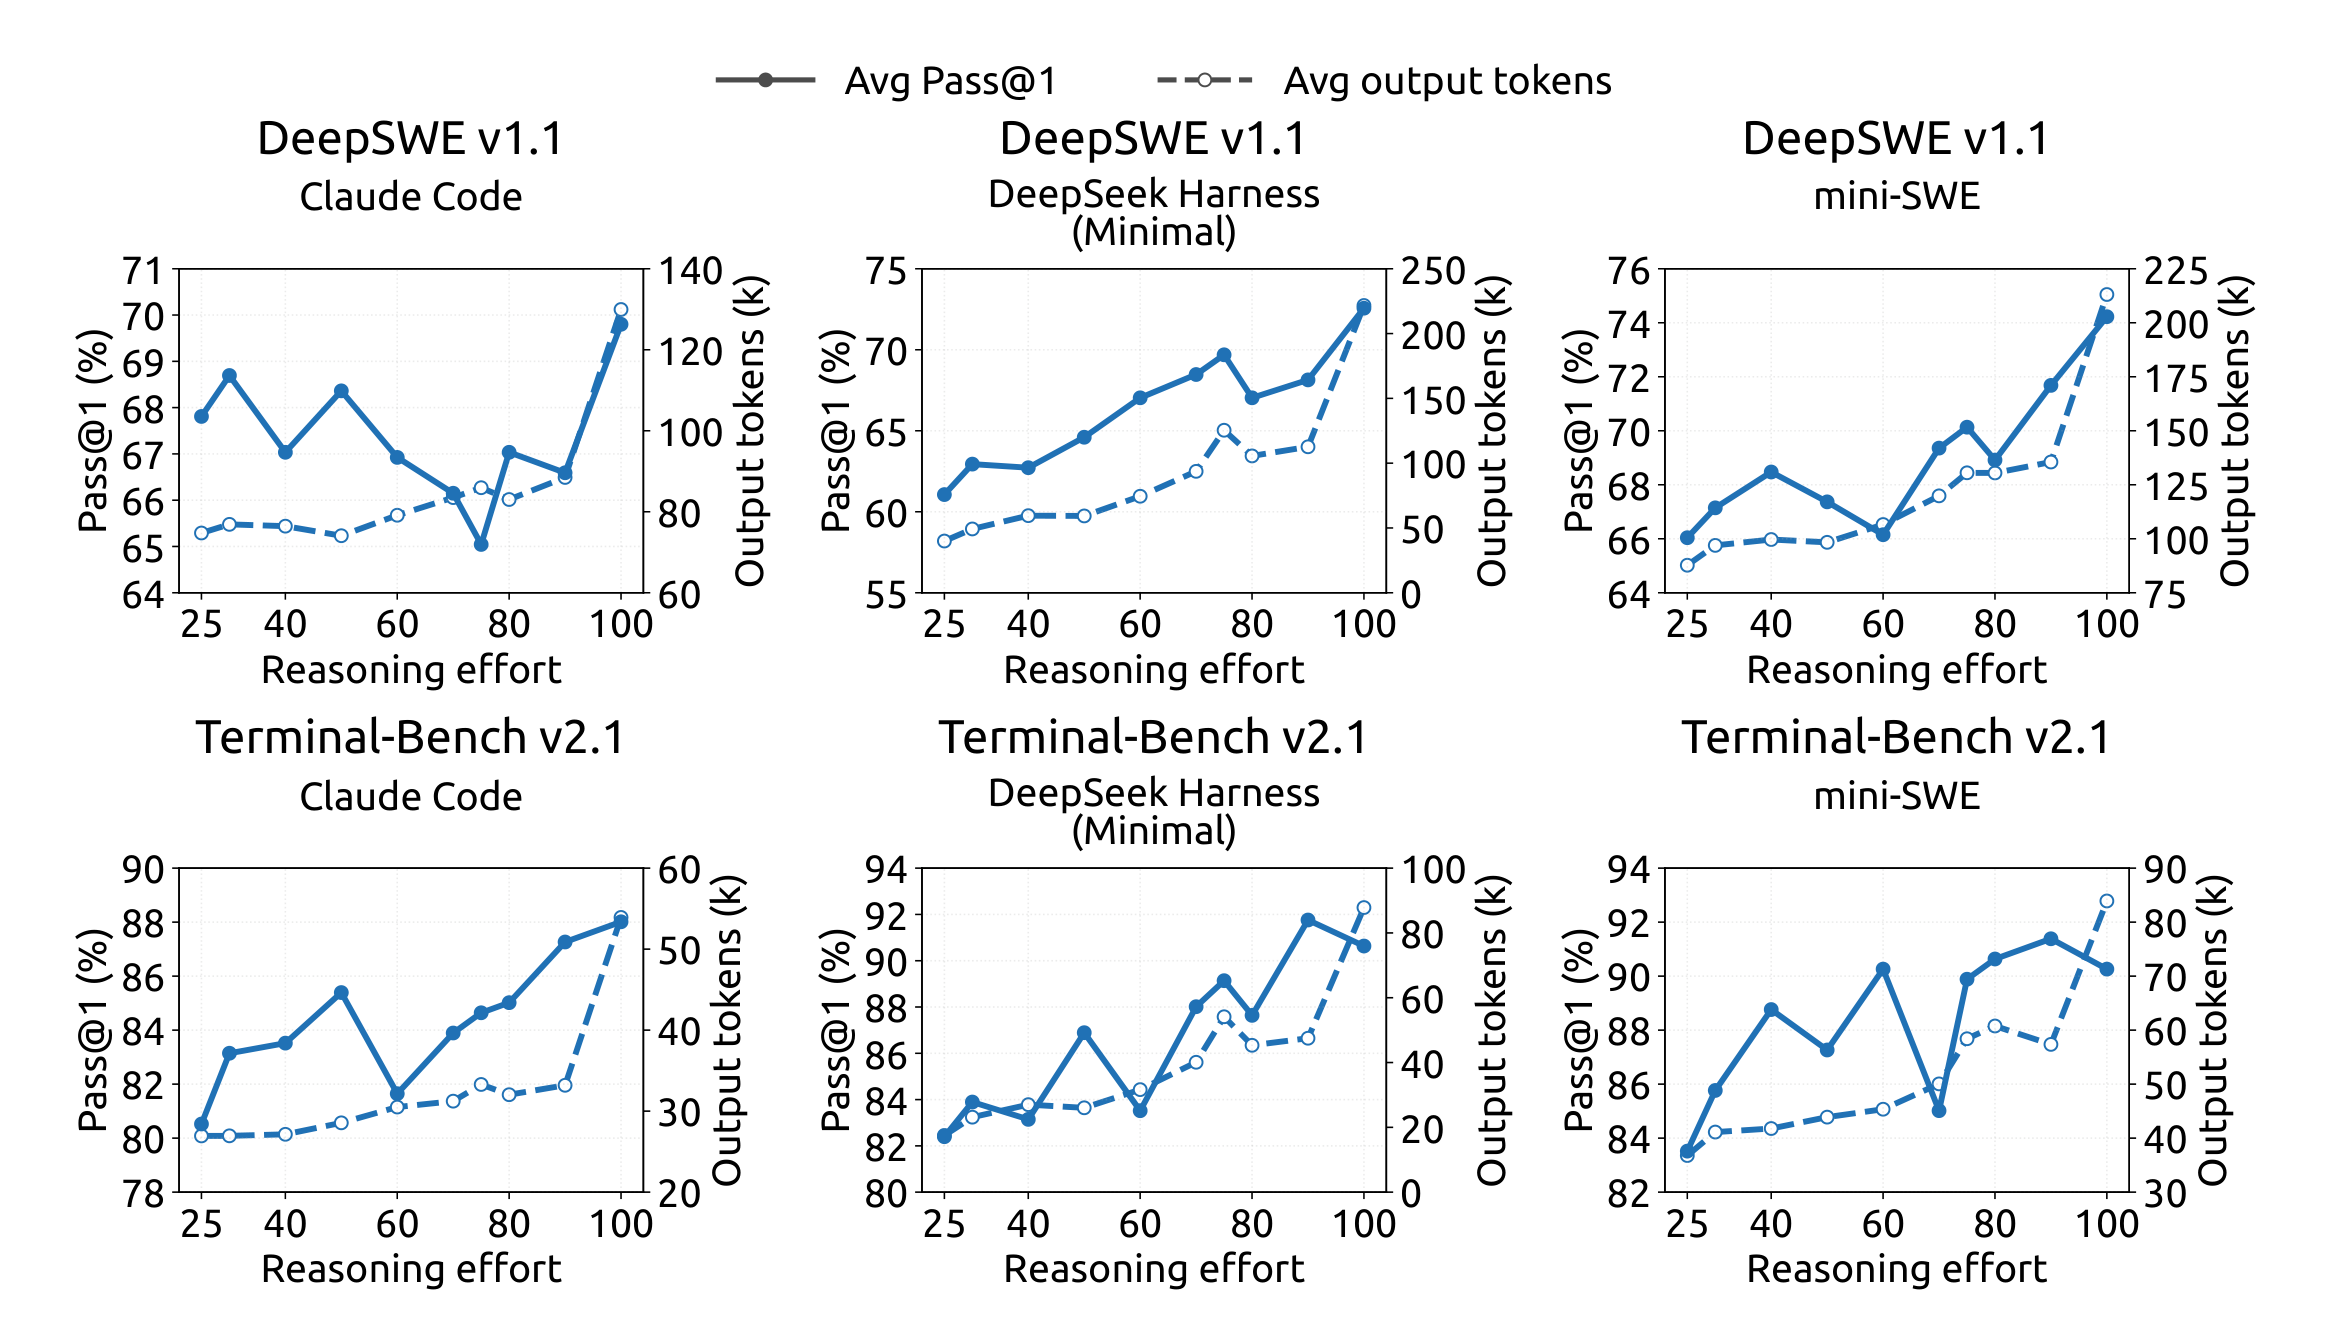
\includegraphics[width=\linewidth]{images_hi/fig11}
\caption{思考强度会一以贯之地拉长轨迹长度，但与各编码脚手架上的准确率仅呈弱相关。每个面板将 Pass@1（\%，实线，左轴）和每条轨迹的平均输出 token 数（k，虚线，右轴）与思考强度设置对应绘图，涵盖 DeepSWE v1.1（上排）和 Terminal-Bench v2.1（下排）在三种智能体脚手架（Claude Code、DeepSeek Harness（Minimal）与 mini-SWE）下的结果。所有面板均来自同一 checkpoint。}
\label{fig:11}
\end{figure}
\begin{figure}[htbp]
\centering
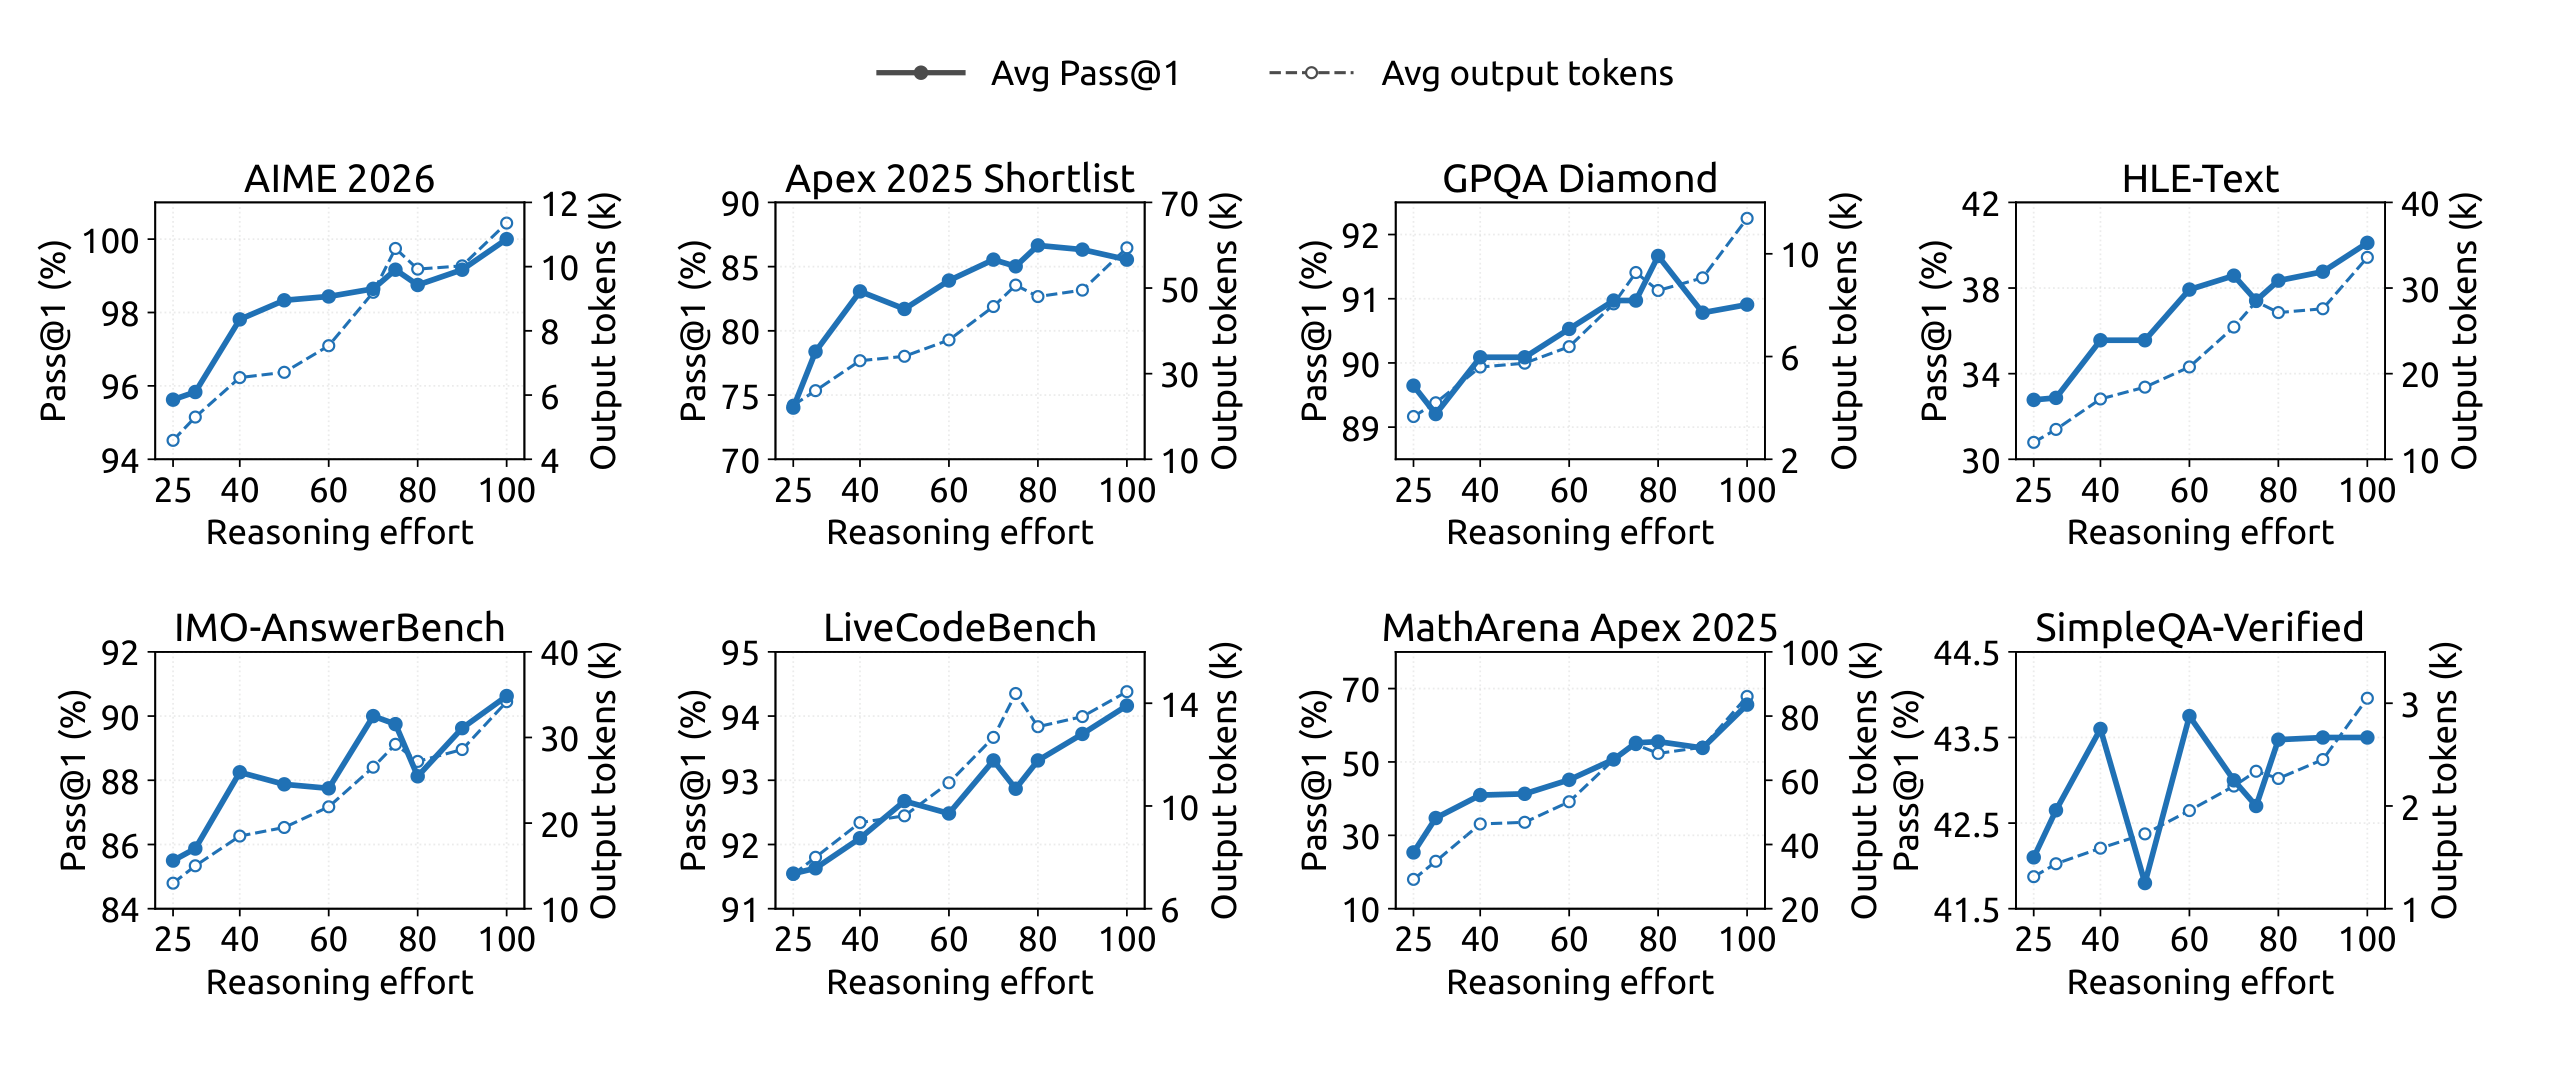
\includegraphics[width=\linewidth]{images_hi/fig12}
\caption{八个推理密集型基准上性能与输出长度随思考强度的变化。每个面板在思考强度取值从 25 变化到 100 时，绘制 Pass@1（实线，左轴）和每条响应的平均输出 token 数（虚线，右轴）。}
\label{fig:12}
\end{figure}

\end{document}
